\providecommand{\classoptions}{keys}
%% The next two lines are suggested at
%% to work around the following error:
%%
%%  ----------------------------
%%  /usr/local/texlive/2018/texmf-dist/tex/latex/chngcntr/chngcntr.sty:42: LaTeX Error: Command \counterwithout already defined.
%%                 Or name \end... illegal, see p.192 of the manual.
%%
%%  See the LaTeX manual or LaTeX Companion for explanation.
%%  Type  H <return>  for immediate help.
%%   ...
%%
%%   l.42 ...thout}{\@ifstar{\c@t@soutstar}{\c@t@sout}}
%%   ----------------------------
%%
%% The two lines:
\let\counterwithout\relax
\let\counterwithin\relax
%% Suggested fix above taken from
%% https://tex.stackexchange.com/questions/425600/latex-error-command-counterwithout-already-defined
%%
\documentclass[noworkareas,deliverables,svgnames,\classoptions]{euproposal}       % for writing
%\documentclass[submit,noworkareas,deliverables]{euproposal}        % for submission
%\documentclass[submit,public,noworkareas,deliverables]{euproposal} % for public version

\usepackage[utf8]{inputenc}
%\usepackage{minitoc}

\usepackage{float}  % used to suppress floating of tables in Resources section.
\usetikzlibrary{calc,fit,positioning,shapes,arrows,snakes}

\addbibresource{bibliography.bib}
% temporary fix due to http://tex.stackexchange.com/questions/311426/bibliography-error-use-of-blxbblverbaddi-doesnt-match-its-definition-ve
\makeatletter\def\blx@maxline{77}\makeatother

%%% institutions
\WAinstitution[id=UPSUD,
        countryshort=FR,
        acronym=UPSud]
        {Universit\'e Paris-Sud}

\WAinstitution[id=SRL,
        countryshort=NO,
        acronym=Simula]
        {Simula Research Laboratory}

\WAinstitution[id=XFEL,
        countryshort=DE,
        acronym=XFEL]
        {European XFEL GmbH}

\WAinstitution[id=QS,
        countryshort=FR,
        acronym=QuantStack]
        {QuantStack}


\WAinstitution[id=QS,
        countryshort=FR,
        acronym=QuantStack]
        {QuantStack}

\WAinstitution[id=INSERM,
        countryshort=FR,
        acronym=INSERM]
        {INSERM}

\WAinstitution[id=SIL,
        countryshort=PL,
        acronym=Silesia]
        {University of Silesia}

\WAinstitution[id=WTT,
        countryshort=CH,
        acronym=WildTree]
        {WildTreeTech}

\WAinstitution[id=UIO,
        countryshort=NO,
        acronym=UiO]
        {University of Oslo}

\WAinstitution[id=EGI,
        countryshort=NL,
        acronym=EGI]
        {EGI}

\WAinstitution[id=CDS,
        countryshort=FR,
        acronym=CDS]
        {Centre de Donn\'ees astronomiques de Strasbourg}

\WAinstitution[id=EP,
        countryshort=FR,
        acronym=EP]
        {Ecole polytechnique}

\WAinstitution[id=XXX,
        countryshort=XX,
        acronym=Template]
        {Template Institution}



% \WAinstitution[id=PD,
%         countryshort=CH,
%         acronym=PersonalData]
%         {PersonalData.io}

\WAperson[id=minrk,
           personaltitle=Dr. ,
           birthdate=9 Oct. 1984,
           academictitle=Research Engineer,
           affiliation=SRL,
           department=Numerical Analysis and Scientific Computing,
           privaddress=None of your business,
           privtel=that neither,
           email=benjaminrk@simula.no,
           workaddress={TODO: Simula, Fornebu},
           %worktel=+33 6 77 90 32 79,
           % worktelfax=+33 6 77 90 32 79,
           %workfax=N/A
           ]
           {Benjamin Ragan-Kelley}

%%% Local Variables:
%%% mode: latex
%%% TeX-master: "proposal"
%%% End:

% LocalWords:  WAperson miko personaltitle academictitle privaddress privtel Sud
% LocalWords:  workaddress worktel workfax gc worktelfax pcg pcsa WAinstitution
% LocalWords:  shortname partof streetaddress townzip countryshort efo 3kd89
% LocalWords:  jacobs-logo.png Seefahrtstrasse Kruislann Montparnasse Universit
% LocalWords:  baz Westerfield
 % Some sections of the included files depend on this.
\usepackage{lscape} % for landscape
\usepackage{comments}
% %\usepackage[final]{comments}
\usepackage{verbatim}
\usepackage{listings}
\usepackage{supertabular,array}
\makeatletter
\newcommand\arraybslash{\let\\\@arraycr}
\makeatother
% \setlength\tabcolsep{1mm}
% \renewcommand\arraystretch{1.3}
%% Related Projects
\newcommand{\scienceproject}{\mbox{\textsc{SCIEnce}}\xspace}
\newcommand{\OOMMF}{OOMMF\xspace}
\newcommand{\OOMMFNB}{OOMMF-NB\xspace}
\newcommand{\ODK}{OpenDreamKit\xspace}
\newcommand{\VRE}{VRE\xspace}
\newcommand{\VREs}{VRE\xspace}
\newcommand{\software}[1]{\mbox{\textsc{#1}}\xspace}
\newcommand{\GAP}{\software{GAP}}
\newcommand{\HPCGAP}{\software{HPC-GAP}}
\newcommand{\libGAP}{\software{libGAP}}
\newcommand{\Singular}{\software{Singular}}
\newcommand{\Sage}{\software{Sage}}
\newcommand{\SageCombinat}{\software{Sage-Combinat}}
\newcommand{\MuPADCombinat}{\software{MuPAD-Combinat}}
\newcommand{\Docutils}{\software{Docutils}}
\newcommand{\Pygments}{\software{Pygments}}
\newcommand{\Sphinx}{\software{Sphinx}}
\newcommand{\SCSCP}{\software{SCSCP}}
\newcommand{\JavaScript}{\software{JavaScript}}
\newcommand{\Python}{\software{Python}}
\newcommand{\IPython}{\software{IPython}}
\newcommand{\Jupyter}{\software{Jupyter}}
\newcommand{\JupyterHub}{\software{JupyterHub}}
\newcommand{\Cython}{\software{Cython}}
\newcommand{\Pythran}{\software{Pythran}}
\newcommand{\Numpy}{\software{Numpy}}
\newcommand{\Pari}{\software{PARI}}
\newcommand{\PariGP}{\software{PARI/GP}}
\newcommand{\libpari}{\software{libpari}}
\newcommand{\GP}{\software{GP}}
\newcommand{\GPtoC}{\software{GP2C}}
\newcommand{\Linbox}{\software{LinBox}}
\newcommand{\LMFDB}{\software{LMFDB}}
\newcommand{\OpenEdX}{\software{OpenEdX}}
\newcommand{\Linux}{\software{Linux}}
\newcommand{\LATEX}{\software{\LaTeX}}
\newcommand{\SMC}{\software{SageMathCloud}}
\newcommand{\cocalc}{\software{CoCalc}}
\newcommand{\Simulagora}{\software{Simulagora}}
\newcommand{\KANT}{\software{KANT}}
\newcommand{\Magma}{\software{Magma}}
\newcommand{\Mathematica}{\software{Mathematica}}
\newcommand{\Maple}{\software{Maple}}
\newcommand{\Matlab}{\software{Matlab}}
\newcommand{\MuPAD}{\software{MuPAD}}
\newcommand{\MPIR}{\software{MPIR}}
\newcommand{\Arxiv}{\software{arXiv}}
\newcommand{\Givaro}{\software{Givaro}}
\newcommand{\fflas}{\software{fflas}}
\newcommand{\MathHub}{\software{MathHub}}
\newcommand{\FindStat}{\software{FindStat}}
\newcommand{\GitHub}{\software{GitHub}}
\newcommand{\GitLab}{\software{GitLab}}
\newcommand{\Trac}{\software{Trac}}
\newcommand{\git}{\software{git}}
\newcommand\DKS{\ensuremath{\mathcal{DKS}}\xspace}
\newcommand{\FLINT}{\software{FLINT}}
\newcommand{\nbval}{\software{nbval}}
\newcommand{\nbdime}{\software{nbdime}}
\newcommand{\nbdiff}{\software{nbdiff}}
\newcommand{\nbmerge}{\software{nbmerge}}
\newcommand{\conda}{\software{conda}}
\newcommand{\anaconda}{\software{anaconda}}
\newcommand{\clang}{\software{clang}}
\newcommand{\gcc}{\software{gcc}}
\newcommand{\cling}{\software{cling}}
\newcommand{\Julia}{\software{Julia}}
\newcommand{\Fortran}{\software{Fortran}}

%%% Local Variables:
%%% mode: latex
%%% TeX-master: "proposal"
%%% End:

\usepackage{framed}

\newcommand{\allparticipants}{{UPSUD,SRL,XFEL,QS,SIL,WTT,UIO,EGI,INSERM,CDS,EP}}

\begin{document}
\begin{proposal}[
  % These PM numbers (person months) are for the coordinator to help planning
  % Participants should not change these, but add PM numbers in the CVS in
  % the site descriptions at CVs/*.tex
  % TODO: Nicolas needs to update these numbers from the (requested ones)
  site=SRL, % Simula
  site=CDS, % CDS
  site=EP, % Ecole polytechnique
  site=EGI, % EGI
  site=XFEL, % European XFEL GmbH
  site=INSERM, % INSERM
  site=QS, % QuantStack
  site=UIO, % U Oslo
  site=UPSUD, %paris sud
  site=SIL, % U Silesia
  site=WTT, % WildTreeTech
  % site=XXX, % template example
  % alternative: (can be combined)
    coordinator=minrk,
  coordinatorsite=SRL,
  acronym={BOSSEE},
  acrolong={BOSSEE},
  proposalnumber={...},
  title=Building Open Science Services\\ on European E-infrastructure,
  callname=Topic: Prototyping innovative services,
  callid=INFRAEOSC-02-2019,
  % TODO: consistency with provided template
  % CALL: H2020-EINFRA-2015-1
  % TOPIC: e-Infrastructures for Virtual Research Environments (VRE)
  % Instrument: e-Infrastructures
  keywords={open science, reproducibility, education, jupyter, binder, cloud, EOSC},
  % computational mathematics,
  % GAP, Linbox, PARI, Sage, Singular, IPython, Jupyter, SageMathCloud, LMFDB, MathHub
  % Virtual research environments, MPIR, /GP
  % open source, free software, number theory, abstract algebra, notebooks
  instrument= Call: INFRAEOSC-02-2019, %Call: H2020-EINFRA-2015-1, 3 Topic 9-2015
  challengeid = TODO,
  %challenge = {N/A},
  %objectiveid={N/A},
  %objective = TODO,
  %outcomeid = N/A,
  %outcome = N/A,
  months=48,
  compactht]
\newcommand{\TheProject}{\pn}% \pn is defined automatically
% \input{grantagreement-history}
\ifgrantagreement
\else
\clearpage
\begin{abstract}
  The Jupyter notebook and Jupyter ecosystem are of increasing
  importance in computational science, data science, in academia,
  industry and services. In addition to supporting high productivity
  of researchers, they have great potential to push open science
  forward: the notebook provides a complete description of a
  computational and data science study, and the notebook can -- in
  principle -- be turned into a publication, or can be used to provide
  the required computation for a part of a publication, such as a
  figure. In this way, the notebook enables reproducibility of complex
  tasks with hardly any additional effort on the user side (if used
  appropriately). The Binder project allows for the execution of such notebooks
  in tailored computational environments, an aspect of reproducibility
  that is not widely supported yet and a great opportunity for improvement to open science practices. Furthermore, for users wanting to
  connect to a local Jupyter notebook server on their machine, or to
  connect to a server somewhere else on the Internet, the users only
  need a webbrowser to display the notebook locally. Because of these
  characteristics, the Notebook is already planned to become an
  important service on the European Open Science Cloud (EOSC), for
  example through the EOSC-04 funded PaNOSC project.

  In \TheProject, we will extend the capabilities of the Jupyter
  tools and ecosystem (such as Jupyter Lab, Widgets, and Binder) to pave
  the way for additional functionality that we view as having great
  importance for the European Open Science Cloud, and Open Science more
  widely. These include development of Jupyter core services to enable
  the generation of advances, improved GUI-like widgets elements in
  the notebook, and an infrastructure providing an archive for reproducible
  and re-usable computational and data science studies.

  Most of the contributing partners have longstanding experience and
  roles in the design and development of the Jupyter ecosystem, and
  deploying services built on these to many users across the globe. Complementary to this core expertise, we
  have integrated partners focussing on the application of the newly
  developed tools from a wide range of disciplines, which can each act
  as demonstrators for the new capabilities,
  and help guide the developments made by the project to serve real-world Open Science use cases
  before they are adopted
  more widely through and by EOSC.
\end{abstract}

%%% Local Variables:
%%% mode: latex
%%% TeX-master: "proposal"
%%% End:

\fi
\ifsubmit\else\setcounter{tocdepth}{4}\fi
\tableofcontents

\begin{draft}
\section*{Outline of Project (for Proposers)}

\TODO{This is the place for various READMEs not included in the final submission}

\subsection*{Vision}

An internal attempt at specifying our vision through short
(unsubstantiated) answers.

\begin{verbatim}

> 1) Who are we?

We are researchers, educators, and developers in and around the Jupyter community
at top research institutions and SMEs throughout Europe.


> 2) What is our goal?

To improve the accessibility of EOSC resources to researchers and the general public,
and improve the accessibility, interactivity, and reproducibility of computational research.


> 2.5) What is our strategy?

Our strategy has four core components:

1. Develop the Jupyter and Binder infrastructure, to improve its utility, maturity, and bring it to broader communities.
2. Operate a European Binder service, with the goal of eventually running on EOSC
3. Demonstrate that these services have value to research communities by developing specific applications in domains ranging widely from physics to life sciences to personal data management
4. Develop materials and run training to educate researchers in the ability to do reproducible computational science using the tools we develop, among others

> 3) From where do we start?

Jupyter is widely adopted in numerous communities and used by millions of researchers worldwide.
JupyterHub is a system for building hosted Jupyter services which is rapidly maturing
and being deployed at numerous universities, businesses, and research institutions.
repo2docker is a tool for automatically building reproducible computational environments using best practices for environment specifications and community standard tools such as Docker, conda, and pip.
BinderHub is software for hosting a web service built on repo2docker and JupyterHub,
where individuals can share reproducible environments for immediate and free interaction by readers in their browser.
mybinder.org is an instance of the BinderHub software,
currently serving thousands of users each day.
There are many communities not yet reached by Jupyter,
and Binder must grow beyond a single deployment.


> 4) How do we connect or differ from other projects?

...

> 5) Why are we excellent?

Jupyter has received the prestigious ACM Software System Award in 2017.
Previous winners include UNIX, TCP/IP, and the World Wide Web.

\end{verbatim}

% \subsection*{Mission statement for the grant}

% Our mission is to promote the next generation of community-developed
% open source software, databases, and services adapted to the needs of
% collaborative research in pure mathematics and applications.

% Our research will cover a wide variety of aspects, ranging from
% software development models, user interfaces \TODO{virtual
%   environments?}, deployment frameworks and novel collaborative tools,
% component architecture, design, and standardization of software
% \TODO{system?} and databases, to links to publication, data archival
% and reproducibility of experiments, development models and tools, and
% social aspects.

% It will consolidate Europe's leading position in computational
% mathematics and build on the remarkable success of the ecosystem of
% projects GAP, Python/Sage, Pari, Singular, LMFDB.

\subsection*{Description of the call}

\verbatiminput{call_description}

% \TODO{What do we mean by ``new generation''}.

\renewcommand{\thepage}{\arabic{page}}
\setcounter{page}{1}
\black
\cleardoublepage
\end{draft}

%%% Local Variables:
%%% mode: latex
%%% TeX-master: "proposal"
%%% End:

%  LocalWords:  verbatiminput renewcommand thepage setcounter cleardoublepage


% ---------------------------------------------------------------------------
%  Section 1: Excellence
% ---------------------------------------------------------------------------

\section{Excellence}
\subsection{Context and motivation}

In many scientific disciplines, it is common for researchers to rely on
heterogeneous computational tools and technologies to collect data,
explore the input data sets, run simulations, visualise the outcome,
and share their result with peers or a with a larger audience. Often,
such data analysis cycles are iteratively refined.

For simple data sets, processes may remain manageable. However, when
dealing with larger and more complex use cases, including big data
from research facilities or High Performance Computing resources, the
complexity makes iteration cycles slower for the researchers. A
complex iteration cycle also makes research results more difficult to
reproduce. Results that are reproducible can much more easily be
re-used in future work.

This situation is exacerbated by the expected increase of the amount
of scientific data being available, including the data becoming
accessible through the EOSC-Hub.


%%HF: the following seemed to be to specialised to list in the opening
%%pararaphs?
%
%which
%is especially harmful in scientific software engineering where most innovation
%is achieved through \emph{incrementalism}.

\subsection{Project Jupyter}
\label{sec:project-jupyter}

\emph{Project Jupyter} \cite{Jupyter}, which has grown increasingly popular in the scientific
computing community, has become the \emph{lingua franca} of interactive
computing in both academia and industry. The main goal of Project Jupyter
project is to provide a consistent set of tools to improve researchers'
workflows from the exploratory phase of the analysis to the communication
of the results \cite{Kluyver2016}.

Started in 2014 from the \emph{IPython Project} \cite{IPython}, Jupyter has grown in
popularity and adoption both in the industry and academia. We estimate the user
base of the Jupyter notebook to be of several millions. Users range from data
scientists to researchers, educators and students from many fields,
including journalists and librarians. In 2017, the Jupyter
team was awarded the \emph{ACM Software System Award}, an annual award that
honors people or an organization "for developing a software system that had a
lasting influence". Prior recipients include \emph{Unix}, \emph{TCP/IP}, and
the \emph{World Wide Web}.

A large number of discrete software components make up Project Jupyter.
While these interact with one another, many can be installed separately
to serve various use cases. For this proposal, we loosely divide the
software involved into \emph{core} components developed under the guidance
of the developers who started the project, and the broader \emph{Jupyter
ecosystem} including software developed by third parties. Some of the
important components and concepts are detailed below.

\begin{figure}[ht]\centering
  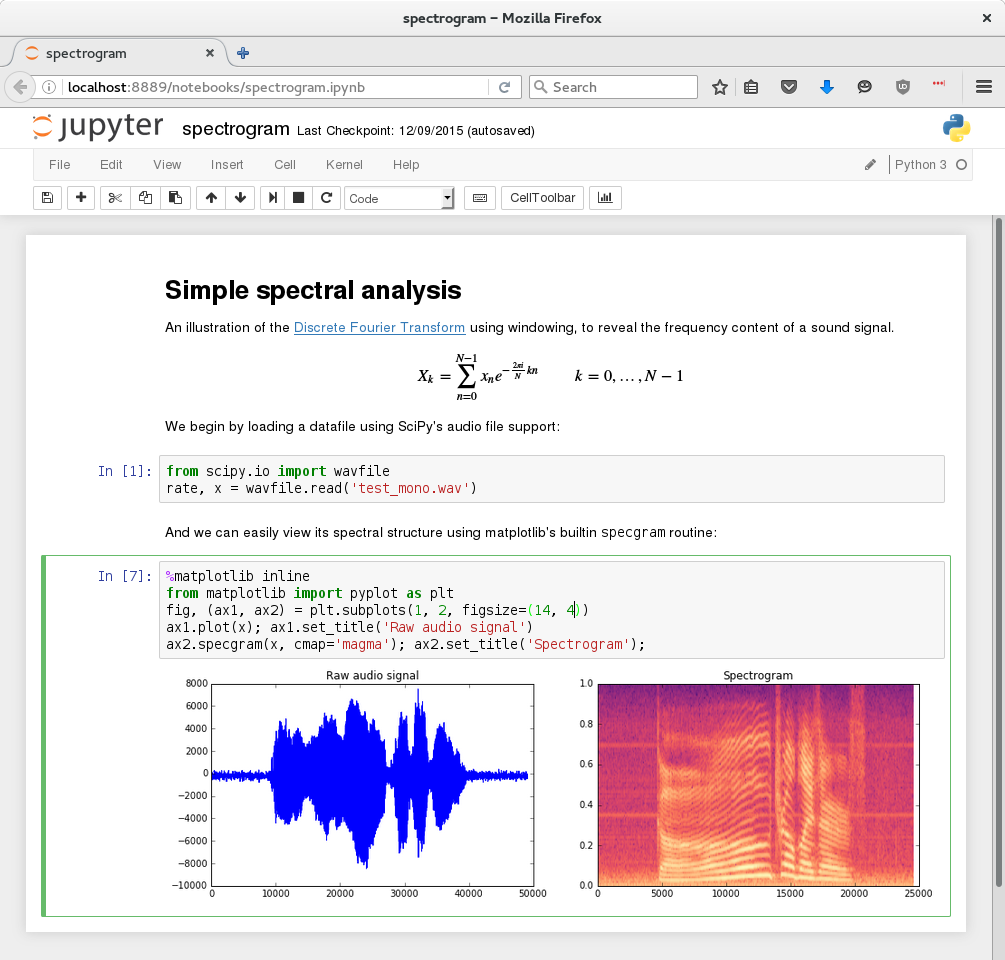
\includegraphics[width=0.9\textwidth]{spectrogram_smaller.png}
  \caption{A notebook document in the Jupyter Notebook interface.}\label{fig:notebook-screenshot}
\end{figure}

\begin{itemize}
  \item The \textbf{Jupyter Notebook} is the flagship application of Project Jupyter.
  It allows the creation of notebook documents, containing a mixture of text and
  interactively executable code, along with rich output from running that code.
  Figure \ref{fig:notebook-screenshot} shows an open notebook including graphs
  from an audio processing example. Notebook documents are readily shareable,
  providing a popular way to describe and illustrate computational methods and
  tools.

  \item \textbf{Jupyter kernels} are the backend software which allow Jupyter to execute
  code in many different programming languages. The \textbf{IPython} kernel is
  the reference kernel, supporting the Python programming language, and is
  developed by the Jupyter core team. Kernels for other languages are maintained
  by third parties.

  \item \textbf{nbconvert} converts notebook files to a variety of other file
  formats, including HTML and PDF, so that the content of a notebook can easily
  be shared with people who don't have Jupyter software. nbconvert also powers
  \textbf{nbviewer}, a web service which provides static HTML views of publicly
  accessible notebooks.

  \item \textbf{JupyterHub} is a multi-user extension of the Jupyter Notebook.
  It runs on one or more servers, for example at a research institution.
  Users can log in to author and run notebooks securely through their web
  browser, without needing to install any special software on their own
  computer.

  \item \textbf{Binder} builds on JupyterHub to allow sharing executable
  notebooks along with (small) data files and a description of the libraries
  required to run the notebooks. When someone accesses a Binder repository,
  the service builds the computational environment on-demand, allowing them to
  execute and modify a copy of the notebooks.
  \textbf{repo2docker} and \textbf{BinderHub} are components of the Binder
  software.
\end{itemize}

\subsubsection{Jupyter ecosystem}

The broader Jupyter ecosystem includes many more projects than we will describe
here, but these are a selection of projects which may be relevant to
\TheProject:

\begin{itemize}
  \item \textbf{nbsphinx} \cite{Nbsphinx} integrates notebooks with the \emph{Sphinx}
  documentation system, which is widely used for software documentation,
  especially but not only for software written in Python.
  This allows developers to write notebooks showing how to use a library,
  then seamlessly make those notebooks part of their main documentation.

  \item \textbf{nbval} \cite{nbval} is a plugin for the popular \emph{pytest} testing
  framework to automatically execute notebooks and optionally check that the
  output matches that saved in the file. While this is not a subsitute for a
  test suite, it's valuable for documentation with code examples in notebooks.
  If changes to the underlying tools mean the example no longer
  works, testing with nbval will quickly show this, so that either the software
  or the example can be corrected. This ensures that example code doesn't
  get outdated.

  \item \textbf{nbdime} \cite{nbdime} provides tools for comparing and merging notebooks.
  These integrate with version control systems such as \emph{git}, which
  are designed for plain text files and typically don't handle notebook files
  well.

  \item \textbf{Widgets} allow interactive output in the notebook which can
  communicate with the kernel, updating values in the kernel and updating the
  displayed output as code runs. \textbf{ipywidgets} \cite{ipywidgets} provides the main
  implementation for the IPython kernel, while other packages such as
  \textbf{bqplot} \cite{bqplot}, \textbf{ipyvolume} \cite{ipyvolume} and
  \textbf{K3D} \cite{K3D} extend the framework to provide 2D and 3D visualisations.
  Figure \ref{fig:ipywidgets-example} shows a simple example of interactive
  widgets in use.

  \item The \textbf{Voila} package \cite{Voila} enables the
  sharing of notebook-based interactive dashboards for non-technical users.

  \item The \textbf{Xeus} instrastructure \cite{Corlay2017} supports writing kernels
  in C++. \textbf{xeus-cling} is one such kernel, running user code in C++,
  and built upon CERN's C++ interpreter, "cling" \cite{Vassilev2012},
  which has a lot of adoption in the High-Energy-Physics community.
  xeus-cling is already in use for teaching the C++ programming language.
\end{itemize}

\begin{figure}[ht]\centering
  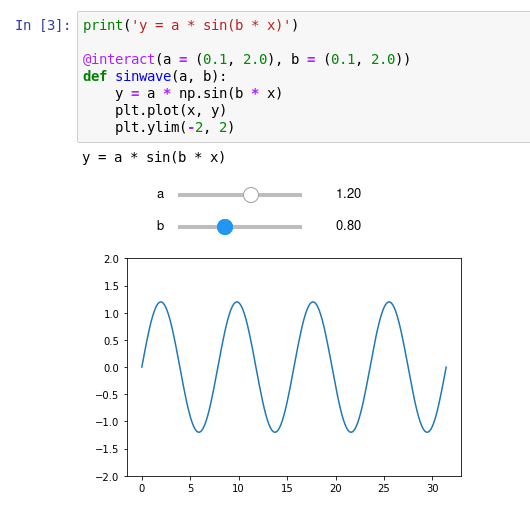
\includegraphics[width=0.6\textwidth]{ipywidgets_example.png}
  \caption{An example of using two simple slider widgets to explore the
  parameter space of a function. The \texttt{@interact} decorator creates
  the widgets and connects them to the function.}
  \label{fig:ipywidgets-example}
\end{figure}

\subsection{This proposal}

In this proposal, core team developers of the project, including a
number of recipients of the ACM award, and key contributors to the
open source scientific computing ecosystem detail improvements to the
capabilities of Project Jupyter.  The goal is to improve the
accessibility of EOSC resources to researchers and the general public,
and improve the accessibility, interactivity, reproducibility and
re-usability of computational research.

\subsubsection{Proposed improvements of core components of Jupyter (WP2)}

We plan to make technical changes to the Jupyter Notebook software to support
real-time collaboration (\taskref{core}{collaboration}),
so that two or more people in different places can work together
on the same notebook. This would significantly enhance the value of
notebooks for collaborative research.
We will also work on making Jupyter software accessible to as broad a
range of users as possible (\taskref{core}{accessibility}).

Further work to bring the code behind JupyterHub and Binder closer together
(\taskref{core}{jh-bh-conv}) will bring a range of benefits, allowing more
flexible sharing of notebooks along with access to remote computing resources
such as EOSC.

Finally, we are explicitly allocating time in \WPref{core} for maintaining
Jupyter software, as well as new development (\taskref{core}{maintenance}).
Maintenance is crucial to creating reliable, sustainable software,
but its cost is often swept under the rug in funding applications
because of the perceived pressure to focus on novelty.

\subsubsection{Proposed improvements of the Jupyter ecosystem (WP3)}

We further propose improvements of the wider Jupyter ecosystem for
better scientific workflows. In particular, we have identified
possible improvements to:

\begin{itemize}
  \item Binder and its crucial software component \emph{repo2docker}
    (\taskref{ecosystem}{r2d-and-binder})

  \item Xeus, to better support the C++ programming language in notebooks
    (\taskref{ecosystem}{xeus-cpp})

  \item Interactive widgets, including tools for 3D visualisation to help
    people make sense of large amounts of data (\taskref{ecosystem}{jupyter-widgets})
\end{itemize}

\WPref{ecosystem} also includes work on tooling and guidelines for using
notebooks in education (\taskref{ecosystem}{teaching-tools}),
and for archiving computational environments to allow reproducible research
with a focus on the long term (\taskref{ecosystem}{reproducibility}).
We may create new open source software projects in these tasks,
but we will carefully review existing existing software, both in the
Jupyter ecosystem and beyond, to avoid unnecessary duplication of effort.

\subsubsection{Beyond the improvement of the Jupyter Project (WP4,
  WP5, WP6)}
Beyond the improvement to the software stack, we plan on
\begin{itemize}
\item Application, demonstration and evaluation of such novel services
  in multiple demonstrators, that cover research fields such as
  health, astrophysics, photon and neutron science, geosciences and
  mathematics, and also interests of participating SMEs (WP4)
\item Operating a \emph{European Binder Service} on the EOSC-hub and
  enabling provision of Jupyter Services through the EOSC-sub (WP5).
\item Producing \emph{training and education material} to disseminate
  the ability to do reproducible computational science using the tools
  we develop, among others. (WP6)
\end{itemize}

\TODO{HF: This is a nice summary. Is that good here in the excellence
  section? Or should we have a separate 'execute summary' before the
  main document starts, that shows the above?}

\clearpage

%%% Local Variables:
%%% mode: latex
%%% TeX-master: "proposal"
%%% End:


\subsection{Objectives}
\label{sect:objectives}
\eucommentary{1-2 pages}
\eucommentary{\emph{Describe the specific objectives for the project,
which should be clear, measurable, realistic and achievable within the
duration of the project. Objectives should be consistent with the expected
exploitation and impact of the project (see section 2).
Desirable keywords: sustainability, impact, reproducibility,
interoperability, ...
}
}

\noindent The aims of \TheProject are:

\begin{compactenum}[\textbf{Aim} 1:]

\item \label{aim:facilitation}
  Facilitate Open Science through the development
  of tools enabling reproducibility, sharing, and collaboration.

\item \label{aim:accessibility}
  Maximise accessibility and interoperability of Open Science services and tools,
  across domains, disciplines, and demographics.

\item \label{aim:sustainability}
  Maximise sustainability of software tools for Open Science
  by developing the community and contributing
  to and supporting community-led software efforts.

\end{compactenum}

\noindent We will achieve our aims through the following objectives:

\begin{compactenum}[\textbf{Objective} 1:]

\item \label{obj:deployment} \TODO{potential title: Generic Jupyter infrastructure and services for the EOSC}%
  Contribute an infrastructure to the European Open Science Cloud
  (EOSC) and the wider Open Science community that can be tailored to
  provide a multitude of generic or specialized services to support
  open science in a wide range of scientific domains and projects.
  This infrastructure will build on the Jupyter project and ecosystem,
  taking the form of a federation of JupyterHub/Binder instances,
  tightly integrated into the EOSC-Hub.

\item \label{obj:jupyter} \TODO{potential title: Supporting and steering the Jupyter ecosystem}%
  Support and steer the Jupyter ecosystem, as a general purpose
  toolbox for better science through interactive computing and
  visualisation that supports the entire life-cycle of open science:
  from initial exploration to publication, research and development in
  industry, teaching, and outreach. In particular, shape and develop
  the Jupyter ecosystem of tools further so that they can become key
  technology for the EOSC-hub.

\item \label{obj:interactivity} \TODO{potential title: Even more interactivity in Jupyter}%
  Improve the interactive capabilities of the Jupyter environment,
  through developments of interactive widgets,
  visualization tools, collaboration features, dashboards,
  and expanded support for kernels such as interactive C++.
  While Jupyter is already widely used, there are many areas
  of interactive exploration that can be improved upon.

\item \label{obj:reusability} \TODO{potential title: Reproducibility and FAIR data}%
  Extend the facilities for reproducibility of computational environments
  and facilitating FAIR data practices.
  We will contribute to the recording and reproducibility
  of environments with repo2docker and Binder
  and extend capabilities to better support FAIR
  data requirements. In particular, the archival of execution
  environments to support re-usability of notebooks in the future
  needs attention. Such notebooks may be published alongside
  publication manuscripts to detail the computation of published data
  and figures, to address the Re-usable requirement of FAIR data.

\item \label{obj:demonstrators} \TODO{potential title: Demonstrators in sciences}%
  Demonstrate and evaluate the  versatility and value of the design and
  the services building on it, through applications to a number of
  domains in academic research, education, research infrastructures, SMEs and for
  the public sector, driven through our project partners. In
  particular, we will contribute demonstrators in the following areas: research infrastructure facilities and
  Photon Science (\site{XFEL}), SMEs (\site{QS}, \site{WTT}),
  astronomy (\site{CDS}), life sciences (\site{INSERM}),
  geosciences (\site{UIO}), physics (\site{SIL}),
  and mathematics and education (\site{UPSUD}, \site{EP}).

\item \label{obj:outreach-and-engagement} \TODO{potential title: Outreach, engagement, and sustainability}%
  Reach out to scientists and the wider Open Science and Open Data
  communities to encourage engagement
  and exploitation of the EOSC-Hub and the Jupyter-based Open Science
  Services for their research domains and interests.
  Engaging a larger community will help ensure the sustainability of
  the services and underlying infrastructure by distributing its
  development, hosting, and maintenance over stakeholders from a
  variety of institutions.

\end{compactenum}

\noindent Progress toward these aims can be monitored via the following
Key Performance Indicators (KPIs):

\begin{compactenum}[\textbf{KPI} 1:]
  \item \label{kpi:workshop-attendees}
    Aim \ref{aim:accessibility}:
    Attendees at Open Science workshops organised by \TheProject participants.
  \item \label{kpi:binder-publications}
    Aim \ref{aim:facilitation}:
    Open publications available on \TheProject services.
  \item \label{kpi:binder-visits}
    Aim \ref{aim:accessibility}:
    Visitors to \TheProject services, engaging with open, interactive communications.
  \item \label{kpi:dissemination}
    Aim \ref{aim:facilitation}:
    Publications and presentations by \TheProject documenting the use of \TheProject services for Open Science.
  \item \label{kpi:contributions}
    Aim \ref{aim:sustainability}:
    Contributions by \TheProject and the wider community to Jupyter software and others.
\end{compactenum}


\TODO{table relating objectives and tasks/deliverables}

\clearpage

\draftpage
% ---------------------------------------------------------------------------
%  Section 1.2: Relation to the work programme
% ---------------------------------------------------------------------------
\subsection{Relation to the Work Programme}


\draftpage
% ---------------------------------------------------------------------------
%  Section 1.3: Concept and Approach
% ---------------------------------------------------------------------------
\TOWRITE{NT/...}{Finalise}
\TOWRITE{ALL}{Proofread concept and approach pass 2}

\subsection{Concept and Approach}\label{sec:concept}
\eucommentary{5-8 pages}
\eucommentary{
-- Describe and explain the overall concept underpinning the project.
Describe the main ideas, models or assumptions involved. Identify
any trans-disciplinary considerations;
-- Describe and explain the overall approach and methodology, distinguishing, as
appropriate, activities indicated in the relevant section of the work programme, e.g.
Networking Activities, Service Activities and Joint Research Activities, as detailed in
the Part E of the Specific features for Research Infrastructures of the Horizon 2020
European Research Infrastructures (including e-Infrastructures) Work Programme 2014-
2015;\\
-- Describe how the Networking Activities will foster a culture of co-operation between the
participants and other relevant stakeholders.\\
-- Describe how the Service activities will offer access to state-of-the-art infrastructures,
high quality services, and will enable users to conduct excellent research.\\
-- Describe how the Joint Research Activities will contribute to quantitative and qualitative
improvements of the services provided by the infrastructures.\\
-- As per Part E of the Work Programme, where relevant, describe how the project will
share and use existing basic operations services (e.g. authorisation and accounting
systems, service registry, etc.) with other e-infrastructure providers and justify why such
services should be (re)developed if they already exist in other e-infrastructures. Describe
how the developed services will be discoverable on-line.\\
-- Where relevant, describe how sex and/or gender analysis is taken into account in the
project's content.}


\begin{figure}[ht]\centering
  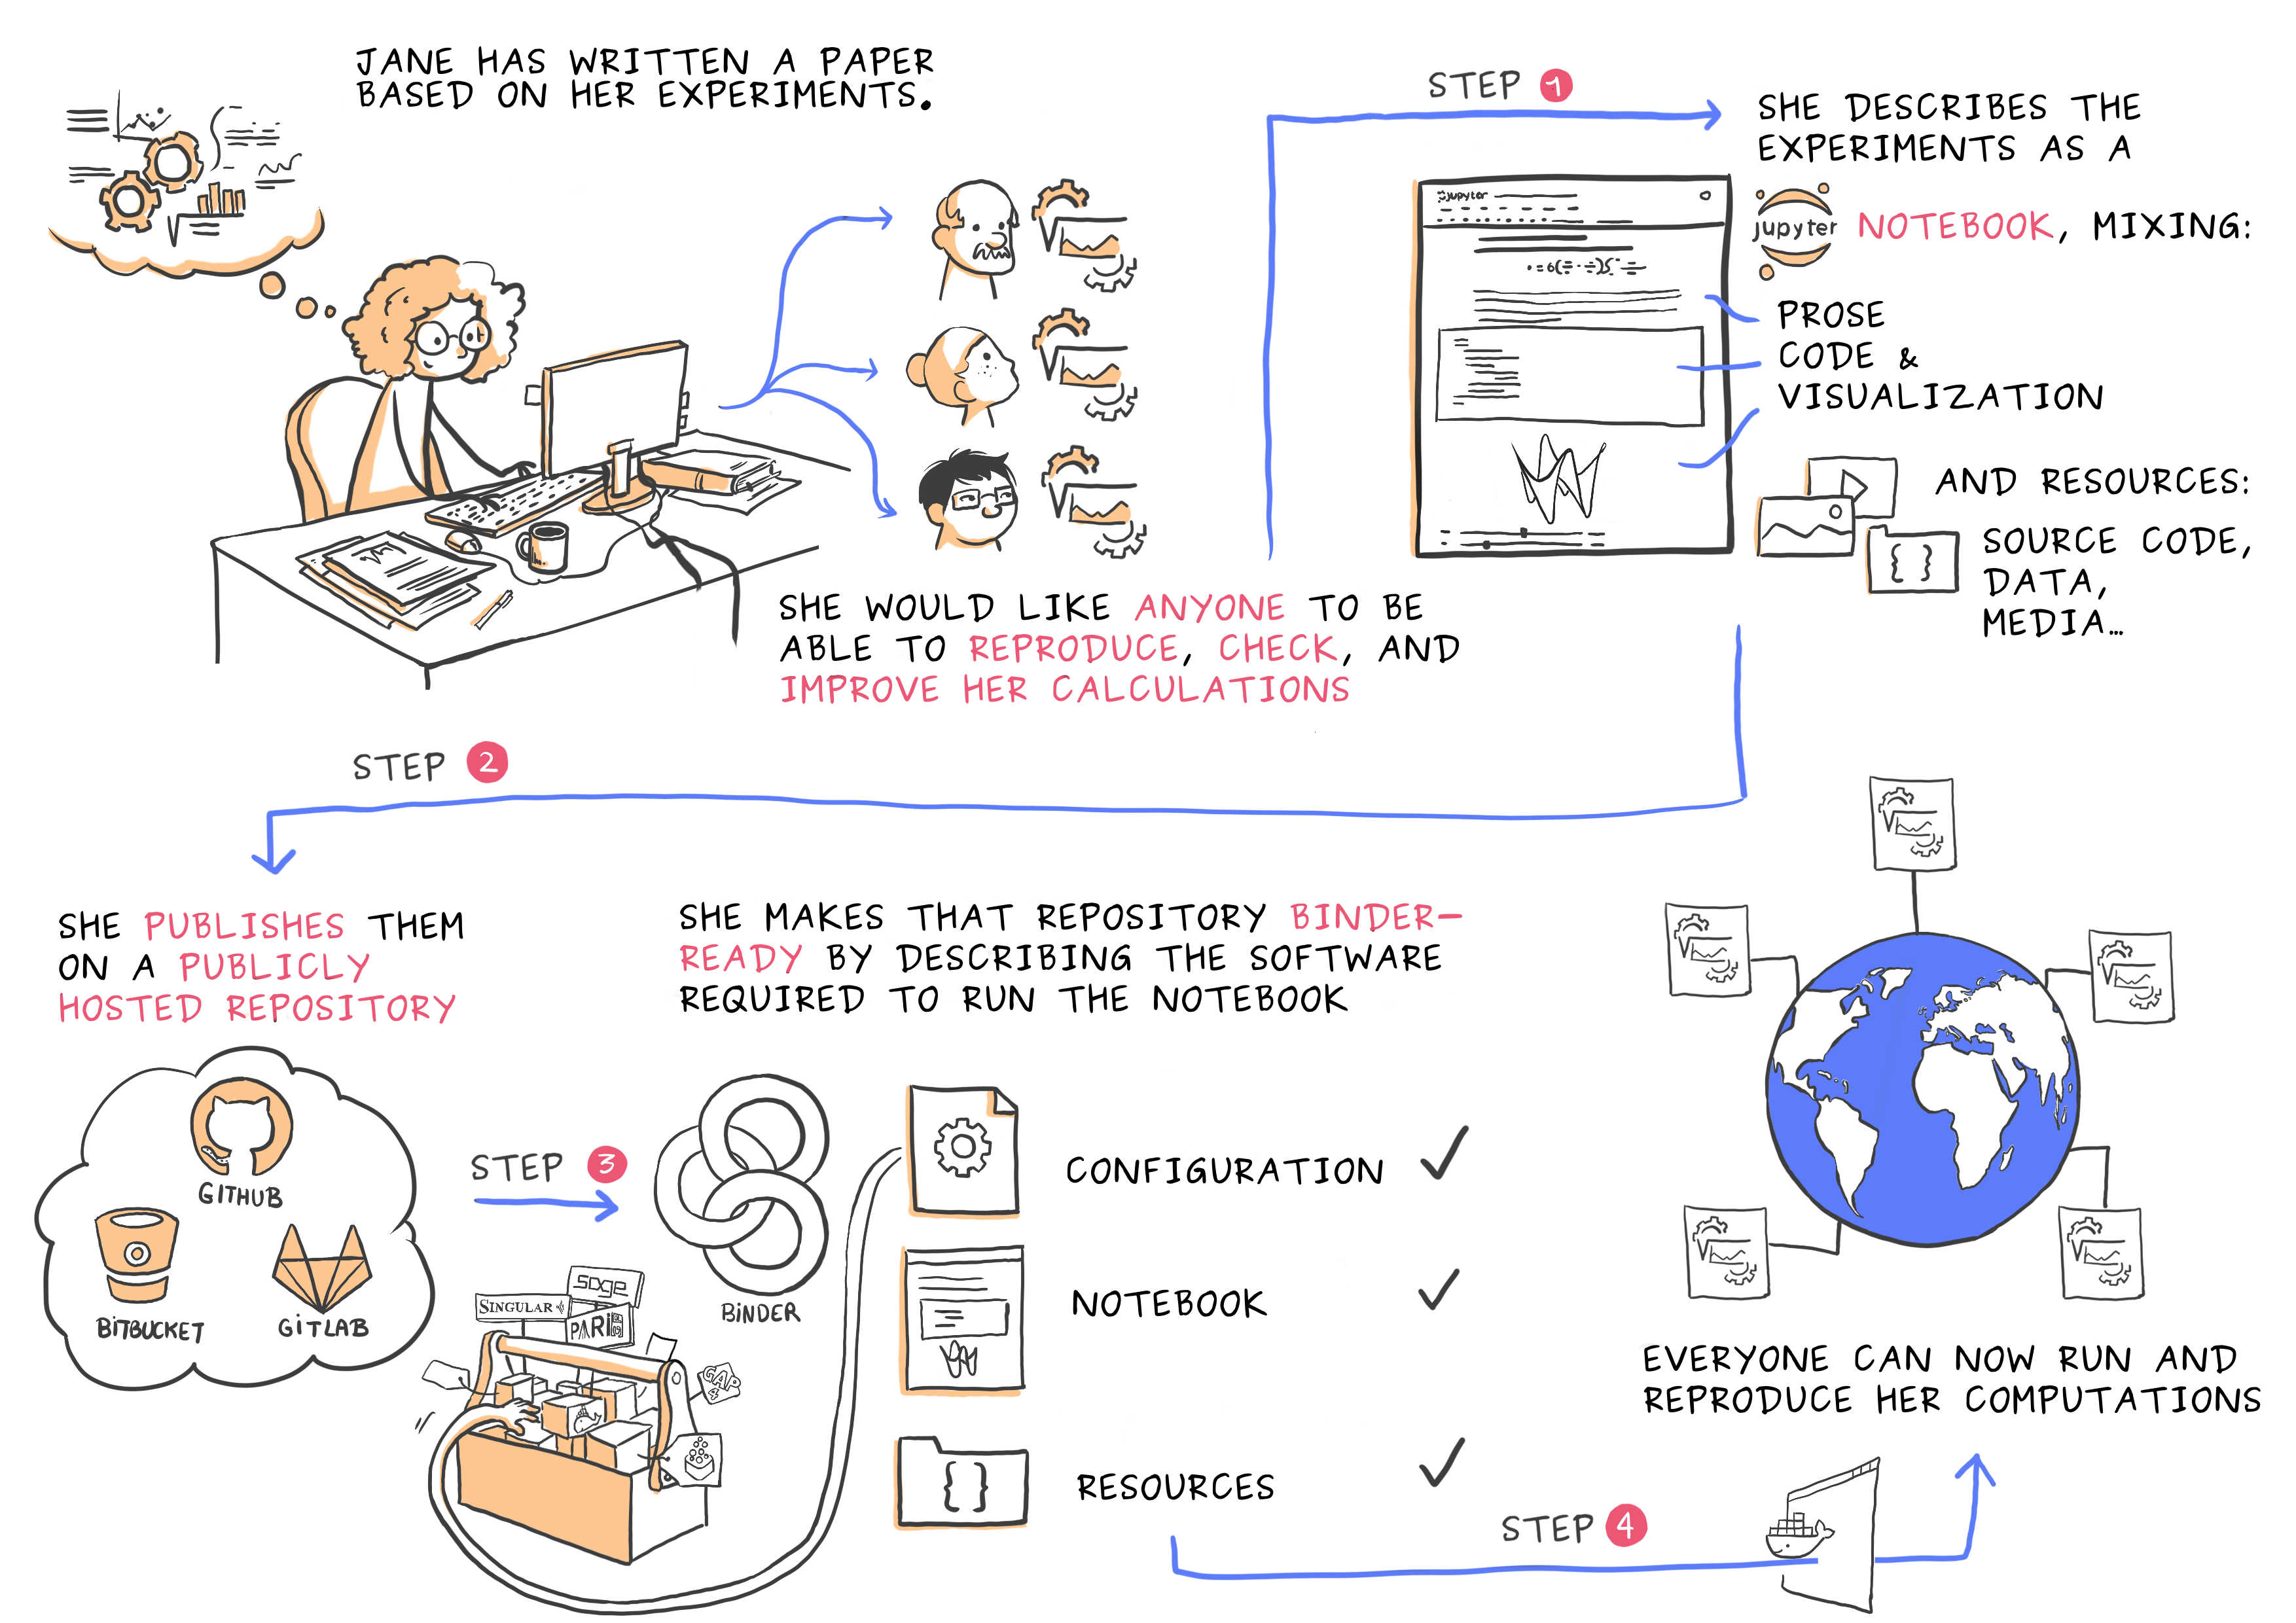
\includegraphics[width=0.9\textwidth]{use-cases-binder-logbook-solution.png}
  \caption{A typical use case for Jupyter notebooks in research.
            Image by Juliette Belin for the OpenDreamKit project, used under
            CC-BY-SA.}\label{fig:use-cases-binder}
\end{figure}

\TODO{
Structure as "The state of the art"
and "Above the art" for what BOSSEE will make better
}

Open Science is the principle that science, in order to be most
impactful and socially responsible, should be done publicly, with as
much of the scientific process and products accessible, reviewable,
and reusable by as many members of the global community as possible.
In the modern age of computational science, almost all academic
fields, from humanities to social sciences to biology and astronomy
are faced with exciting opportunities for Open Science.  As more and
more research takes the form of code and/or data, the opportunity to
share, reproduce, and reuse scientific work is greater than ever, even
enabling new forms of interdisciplinary collaboration.

At the same time as we share in these exciting opportunities, there
are corresponding challenges, technical and social, to making Open
Science a practical reality.  We face big questions: If a researcher
has code and/or data to publicise, how is that best done?  How do
researchers learn best Open Science practices in their field?  How do
previously disconnected fields benefit from each other's work as the
same computational challenges are faced again and again by different
communities?

These are the questions that guide \TheProject.
With so much research being done that wants to be Open,
how can we make Open Science

\begin{enumerate}
    \item as easy as possible to share?
    \item as useful as possible to other researchers and the public?
\end{enumerate}

\noindent Our plan for improving access and effectiveness of Open Science can be summarised as:

\begin{enumerate}
\item improve and maintain common software infrastructure used for
  Open Science
\item develop the Jupyter ecosystem to improve capabilities better
  serve Open Science
\item guide, validate, and demonstrate our developments through
  collaboration with a wide variety of application domains
\item enable students and researchers to perform Open Science through
  training and education, and improving inclusiveness by focusing
  these on under-served and under-represented communities.
\item operate services to facilitate Open Science collaborations with
  Jupyter software
\end{enumerate}

\textbf{Why Jupyter?}

\TheProject has chosen to centre its efforts on the Jupyter software
ecosystem.  The Jupyter notebook and Jupyter ecosystem is of
increasing importance in computational science and data science, in
academia, industry and services. In addition to supporting high
productivity of researchers, they have great potential to push open
science forward: the notebook provides a complete description of a
computational and data science study, and the notebook can -- in
principle -- be turned into a publication, or can be used to provide
the required computation for a part of a publication, such as a
figure. In this way, the notebook enables reproducibility of complex
tasks with hardly any additional effort on the user side (if used
appropriately). The Binder project allows to execute such notebooks in
tailored computational environments; an aspect of reproducibility that
is not widely supported yet. Furthermore, for users wanting to connect
to a local Jupyter notebook server on their machine, or to connect to
a server somewhere else on the Internet, the users only need a
webbrowser to display the notebook locally. Because of these
characteristics, the Notebook is already planned to become an
important service on the European Open Science Cloud (EOSC), for
example through the EOSC-04 funded PaNOSC project.

\TOWRITE{}{short definition of Jupyter components, mixing code \& prose, etc. }

Because the Jupyter notebook is a web-based application, it can be
deployed at computational facilities or in the cloud, and can function
as the basis for services exposing computational resources of all
kinds to researchers and the public.  Because Jupyter is
\textit{interactive}, it enables making scientific results and
communications more interactive than static publications.  The
audience can follow their own initiative and ask their own questions
of published data without needing support from the publishing author,
greatly facilitating the \textit{practicality} of Open Science.

\textbf{Jupyter is generic} \TheProject chose Jupyter because it is
Generic.  Jupyter makes no domain-specific or even language-specific
assumptions.  Any application where mixing description, code, and
results is valuable can make use of Jupyter.  This broad applicability
makes investment in the Jupyter ecosystem extremely effective, because
improvements to Jupyter can serve many communities simultaneously.

Jupyter is built from a collection of standard protocols and file
formats.  Jupyter is not just a single, monolithic collection of
software, but a description of how such software can be built.  The
result is the ability for a variety of communities and applications to
use pieces of Jupyter for their purposes, and/or reimplement pieces to
meet their needs.

For example:

\begin{enumerate}
\item The notebook file format is a well-specified JSON document,
  which can be interpreted by many systems.  This has facilitated the
  development of different services rendering notebooks, e.g. the code
  hosting website GitHub, which renders notebooks for easy viewing by
  anyone, without Jupyter software.
\item the Jupyter protocol describes how execution is performed, which
  has enabled the development of over one hundred kernel
  implementations in dozens of languages.
\item output in the Jupyter protocol uses web-standard MIME types,
  enabling any possible format to be an output in a Jupyter notebook.
\item the JupyterLab extension system provides a system for building
  applications from Jupyter components and others
\item the Jupyter Widgets provide a system for customizing and
  extending interactivity in Jupyter-based environments
\end{enumerate}

The popularity of Jupyter, with millions of users and hundreds of open
source contributors, indicates the value and impact of this approach.

\textbf{How do we improve Jupyter?}

The benefits of focusing our work on a mature system like Jupyter are

\begin{itemize}
\item vibrant community ensures health and sustainability
\item large existing user base maximises impact of contributions
\item mature software ecosystem maintains quality software through
  industry standards such as version control, tests, continuous
  integration, stable release cycles, roadmaps, and user support
\end{itemize}

The Jupyter community aims to be inclusive, and \TheProject will
continue this effort.  Jupyter is inclusive across a number of axes.
By being applicable across numerous domains, Jupyter and \TheProject
encourage participation from individuals of various interests and
backgrounds, and has taken action to improve diversity in the project
by participating in "Outreachy," a program of paid internships for
individuals from groups that face under-representation, systemic bias,
or discrimination.  Jupyter has also operated workshops focused on
training contributors from under-represented groups.  In being free,
public, open source software, Jupyter and \TheProject are accessible
to as many individuals as possible, and invites users and contributors
beyond origin, nationality, beliefs, orientation.  One area where
Jupyter has lacked in this regard is in the User Interface
accessibility, and we will help improve this in
\taskref{jupyter-core}{accessibility}.  Additionally, the project will
focus some of its workshops in \taskref{education}{workshops} on
under-represented communities.


\TODO{
  Architecture diagram of BOSSEE-related software
}

\begin{verbatim}
Outline notes:

* Carry on with specified protocols and formats so that components can be replaced, combined etc.
* Avoid lock-in to specific technologies (for example JupyterHub not limited to AWS but cloud-provide agnostic way) – thus independent from dominating commercial cloud services provider
* Integrating user input in multiple ways
   * User input at JupyterCon: beginners and experience users to try new version of UI; sessions where recorded and used to improve software (“usability testing”)
   * Co-design: developed by scientists for scientists, but professional software engineers and UX designers involved in the design of the software; [deliberate effort because Jupyter is a tool to teach beginners and specialists]
   * UI is at level of polish that is rarely met in non-commercial applications
\end{verbatim}


\draftpage
% ---------------------------------------------------------------------------
%  Section 1.4: Ambition
% ---------------------------------------------------------------------------
\TOWRITE{ALL}{Proofread 1.4 Ambition pass 2}

\subsection{Ambition}

\eucommentary{1-2 pages}

\eucommentary{-- Describe the advance your proposal would provide
  beyond the state-of-the-art, and the extent the proposed work is
  ambitious. Your answer could refer to the ground-breaking nature of
  the objectives, concepts
  involved, issues and problems to be addressed, and approaches and methods to be used.\\
  -- Describe the innovation potential which the proposal
  represents. Where relevant, refer to products and services already
  available, e.g. in existing e-Infrastructures.}

BOSSEE's ambition is to improve the global accessibility of scientific
tools and data, enabling collaboration among researchers and between
researchers and the public.  The world's computational resources are
constantly growing and science is producing ever-more useful and
interesting data.  But how do we enable the European and global
communities to make use of that data?  And not just researchers, but
the public as well?  Open science is a principle of making research
results as broadly accessible and useful as possible.  The first,
minimal step for this is making publications free to access.  The
second step for computational research is to make code and data
publicly accessible, enabling transparency and facilitating
reproducibility and verifiability of results.  But merely making these
resources technically available is not the best we can do.  There can
be many challenges with software, such as environment specifications
and resource requirements, that can be an impediment to the transition
from `technically available' to `practically useful.'  With the tools
of the open source open science community and the resources of the
European Open Science Cloud, we can do better.

The \Jupyter ecosystem consists of a large, global community of
developers and researchers producing software focused on interactive
computation and communication, and is widely used by millions of
individuals in numerous scientific fields, ranging from molecular
biology \cite{Wang2016} to materials science \cite{Hughes2014},
astronomy \cite{Baron2017} and climate science
\cite{Laken2015,Laken2015b}.  \Jupyter software is permissively
licensed under the Berkeley Software Distribution (BSD) license,
allowing anyone to use Jupyter software for free, and even build
derivative commercial products, as has been done in the cases of
Google Colaboratory, Microsoft Azure Notebooks, IBM Watson Studio, and
others \TOWRITE{cite}.  By contributing to the \Jupyter ecosystem,
\TheProject maximises its impact, immediately benefiting the existing
large \Jupyter community, and increasing the likelihood that
\TheProject's results will be maintained by the community after the
end of formal funding.

When it comes to \Jupyter and Open Science, we aim to improve the
\textit{status quo} by bring the two together:

\begin{itemize}
\item Improving software in the Jupyter ecosystem to better serve open
  science.
\item Enable researchers and the public to better perform and benefit
  from open science, through software, services, and education.
\end{itemize}

Open Science that truly benefits society must be more than merely
technically accessible.  Individuals must be able to find the
resources they want and interact with them.  Ideally, they should be
able to ask new questions of models and data published by those that
came before.  This is where \TheProject fits in.  Excellent research
is being performed in all scientific fields, but making those results
practically accessible and engaging to others is a challenge.
\Jupyter notebooks enable publishing code and data in a form that is
interactive, where readers can see code, run it, and see results.
They can then modify the code and produce new data and charts that the
first authors may not have considered.  \Jupyter does not solve the
software installation problem, however, which can be significant for
scientific software.  For a publication to be truly interactive or
reproducible, it must include a computational environment (or a
sufficiently precise description of one such that it can be recreated)
in order to reliably be able to run for another individual.  Services
and tools such as Binder and repo2docker facilitate this.  By
publishing a description of the requirements to run the software,
repo2docker is able to recreate a computational environment with
everything needed to run the software, including a \Jupyter
environment for interactively exploring the resource.  Binder wraps
this in a web service, enabling immediate, free sharing of
computational results on the web, with no requirements of readers
other than a web browser.  By deploying Binder or similar services on
EOSC infrastructure, EOSC enables researchers to make their results
available to the public, and enables the public to interact with the
science they are funding.

All together, \Jupyter and Binder enable the migration of the open
science community from static publication to truly interactive,
reproducible publications.

\TOWRITE{NOTES}

points to hit:

\begin{itemize}
    \item practical reproducibility
    \item interactive publications
    \item environments
    \item builds on opendreamkit
    \item jupyterhub
    \item binder + repo2docker
    \item demonstrators
    \item educating the public
\end{itemize}


%%% Local Variables:
%%% mode: latex
%%% TeX-master: "proposal"
%%% End:

%  LocalWords:  eucommentary textsuperscript textregistered textsuperscript specialised
%  LocalWords:  textregistered recomputation textbf textbf rigourous centred flagshsip
%  LocalWords:  subsubsection realisation textit


\draftpage
% ---------------------------------------------------------------------------
%  Section 2: Impact
% ---------------------------------------------------------------------------
% ---------------------------------------------------------------------------
%  Section 2: Impact
% ---------------------------------------------------------------------------


\section{Impact}
\label{sec:impact}
\TOWRITE{ALL}{Describe impact}

The central impact of the \TheProject project will be a significant improvement
and extension of the Jupyter tools and ecosystem described in section \ref{sec:project-jupyter}
to facilitate open science and reproducible research,
and their wide availability on the European Open Science Cloud.
While this will initially be developed alongside applications for our
own institutions, we expect the tools we develop to be useful to a much larger
group of researchers, as data analysis and simulation are now crucial parts
of many scientific disciplines.

Jupyter-based technology will be especially valuable given the decentralised
nature of EOSC. Large-scale experiments often produce so much data that it is
impractical to transfer the data to another site for analysis.
At European XFEL, for instance, hundreds of terabytes of data may be recorded
for a single user experiment. The analysis steps thus need to run where the
data is stored, even if the scientist has returned to their home institution
far away. As the Jupyter Notebook interface runs in a web browser,
it is readily usable for remote access.

In addition, \TheProject will produce highly visible demonstrations of
notebooks for open science in targeted scientific disciplines.
The result will be innovative new prototype services that will provide
direct benefits to the early adopters in various research fields.
Moreover it will serve as a demonstration of a strategy for open science
using notebooks that will be applicable across many domains.

\subsection{Expected Impacts}

\eucommentary{Please be specific, and provide only information that applies
to the proposal and its objectives. Wherever possible, use quantified
indicators and targets.\\
Describe how your project will contribute to:\\
-- the expected impacts set out in the work programme, under the relevant topic
(including key performance indicators/metrics for monitoring results and impacts);\\
-- improving innovation capacity and the integration of new knowledge
(strengthening the competitiveness and growth of companies by developing
innovations meeting the needs of European and global markets; and, where
relevant, by delivering such innovations to the markets;\\
-- any other environmental and socially important impacts (if not already
covered above).\\
Describe any barriers/obstacles, and any framework conditions (such as
regulation and standards), that may determine whether and to what extent
the expected impacts will be achieved. (This should not include any risk
factors concerning implementation, as covered in section 3.2.)}

The expected impact of \TheProject with respect to the
work program is detailed in the table below.

\begin{center}
\begin{tabular}{|m{.3\textwidth}|m{.7\textwidth}|}\hline
  Expected impact & \\\hline


  Integrating co-design into research and
  development of new services to better support scientific, industrial and
  societal applications benefiting from a strong user orientation &
  The Jupyter tools have always been driven by a close connection to users; since
  the project began as IPython in 2001, many of the developers have been
  scientific researchers using the tools as they developed them. More recently,
  when Jupyter has benefited from dedicated developer time, developers have
  remained in academic institutions, in the kind of role now referred to as
  'research software engineers', allowing day-to-day interactions with
  researchers using Jupyter in a wide range of fields.

  By supporting developers in various research institutions where the improvements
  will be used as they are developed, \TheProject will continue this invaluable
  collaboration.

  The improvements and extensions of the core parts of the Jupyter system are
  being ``co-designed'' by technical, industrial and scientific experts in the
  BOSSEE project, so that they will be widely applicable in new innovative
  services across many scientific disciplines.
  The impact of this approach for enabling scientific use of notebooks is expected
  to be very high because it is a direct response to the strong demand from
  scientists for improving the productivity and reproducibility of their work.
  The notebook approach is being embraced in many scientific disciplines, so the
  proposed services to be developed in BOSSEE are strongly oriented to the user needs.

  \TOWRITE{ALL}{More about impact of Jupyter ecosystem improvements...}
  \\\hline

  Supporting the objectives of Open Science by
  improving access to content and resources, and facilitating interdisciplinary
  collaborations &
  Jupyter notebooks have seen rapid uptake in many kinds of research,
  because they bring together the essential elements of the modern scientific
  computational workflow (from data collection to publication and open sharing)
  in the familiar format of a scientific notebook, with powerful functionality
  for access to scientific content, for analysis and visualisation.
  Notebooks also embody the core concepts of open science by providing a
  mechanism to reproduce results in publications, and collaborative
  sharing of not just scientific results, but of the code that produced them.

  We expect the use of notebooks in EOSC to improve access to scientific code,
  and the data which it handles. By combining code and explanation in a convenient
  digital document, notebooks encourage publishing workflows, whereas code in
  scripts or manual interactive workflows are often kept by the researchers who
  performed them. The focus on clarity and reproducibility also helps to ensure
  that data is meaningfully accessible, by preserving essential understanding to
  make sense of the raw data.

  We have already seen a good example of the Jupyter ecosystem facilitating an
  interdisciplinary collaboration: the LIGO scientific collaboration shared
  notebooks detailing the data processing steps which led to the discovery of
  gravitational waves, using the Binder service to allow anyone to re-compute
  the published plots. Scientists with no background in gravitational waves
  studied these notebooks and improved the signal processing.
  In this proposal, we want to provide this ability to a wider audience through
  EOSC, including for disciplines which rely on processing much larger volumes of
  data. \TOWRITE{ALL}{Citation for the LIGO story?}

  The astronomy application in \TheProject (\taskref{applications}{astro})
  is designed to provide a new level of interoperability of
  reference astronomy data within jupyter notebooks.
  By connecting new notebook capabilities to existing and highly used services,
  we expect to have impacts for the users and also for the service provider.
  The scientific users will have access to new capabilities,
  and we anticipate adoption of new innovative ways of using the data.
  We also expect an impact on the services themselves, in terms of usage,
  but also in terms of capturing precious information and feedback on
  how to evolve these services to best support open and collaborative use of
  the data and services.

  \TOWRITE{ALL}{More impacts for other applications/demonstrators ...}
  \\\hline

  Fostering the innovation potential by opening up
  the EOSC ecosystem of e-infrastructure service providers to new innovative
  actors &
  Jupyter is a collection of open source software built around openly documented
  protocols and formats, along with familiar technologies such as HTML and the
  Python programming language. It's easy for third parties to create new
  tools and services using and integrating Jupyter, as evidenced by the thriving
  ecosystem of tools already in development, both by commercial and non-commercial
  actors. To highlight just one example, the first version of the popular Binder
  service was developed by a group at the Howard Hughes Medical Institute,
  working independently of the core Jupyter maintainers, but building on the
  powerful capabilities provided by Jupyter.

  By bringing the diverse expertise of the BOSSEE partners together in this
  common project, we expect a high impact in terms of enabling a new level of
  integration of scientific, technical and industrial interests for the common
  goal of open science.

  \TOWRITE{ALL}{More on innovation, in particular interaction of participating
  SMEs with scientific and technical partners… opening up EOSC ecosystem to new
  actors who bring new expertise as necessary for enabling technical platforms
  for open science.}
  \\\hline

\end{tabular}
\end{center}


\subsection{Measuring impact}

\TOWRITE{ALL}{Communicating the results, all deliverables

Performance indicators
Monitoring use of prototype services… counting numbers of notebooks created/used/sessions ?? }

\subsection{Barriers, Obstacles and Framework conditions}

The BOSSEE project will certainly face a number of challenges as it undertakes
the ambitious program of work described by this proposal.
We can identify a number of potential barriers and obstacles but overall
these are assessed to be minor and planning is in place to mitigate the
identified risks.

\TOWRITE{ALL}{Identify a few potential barriers and mitigating activities...}

While a number of the partners have worked closely together in previous projects,
the integration of new partners from different disciplines will require
dedicated efforts for communication within the project.

\subsection{Socially important impacts}

\TOWRITE{ALL}{...}

\subsection{Exploitation and Dissemination plans}

\TOWRITE{ALL}{
  table on exploitation plan and dissemination plan (general and per partners). Develop impact at european level and add a business plan to place BOSSEE in the european economic context.
}


\clearpage

% ---------------------------------------------------------------------------
%  Section 3: Implementation
% ---------------------------------------------------------------------------

\section{Implementation}
\COMMENT{Typical granularity: 5-8 work packages with 3-5 tasks and one
  deliverable per task; 10 milestones}

\subsection{Work Plan --- Work packages, deliverables and milestones}
\label{sect:workplan}

\eucommentary{Please provide the following:\\
\begin{compactitem}
\item
brief presentation of the overall structure of the work plan;
\item
timing of the different work packages and their components (Gantt chart or similar);
\item
detailed work description, i.e.:
\begin{compactitem}
\item
a description of each work package (table 3.1a);
\item
a list of work packages (table 3.1b);
\item
a list of major deliverables (table 3.1c);
\end{compactitem}
\item
graphical presentation of the components showing how they inter-relate (Pert chart or similar).
\end{compactitem}
}

\subsubsection{Overall Structure of the Work Plan}\label{sec:workplan-structure}
\ifgrantagreement
The
\else
As shown in Figure~\ref{fig:wplist}, the
\fi
work plan is broken down into
X work packages: \WPref{management}...

\subsubsection{How the Work Packages will Achieve the Project Objectives}
\label{sssec:how_the_work_packages_will_achieve}

% (Section~\ref{sect:objectives},page~\pageref{sect:objectives})
...


\gantttaskchart[draft,xscale=.33,yscale=.33,milestones]

\ifgrantagreement\else
\newpage
\subsubsection{Deliverables}\label{sec:deliverables}
\inputdelivs{9.3cm}
\fi

\newpage
\subsubsection{Milestones}\label{sec:milestones}
\eucommentary{Milestones means control points in the project that help to chart progress. Milestones may
correspond to the completion of a key deliverable, allowing the next phase of the work to begin.
They may also be needed at intermediary points so that, if problems have arisen, corrective
measures can be taken. A milestone may be a critical decision point in the project where, for
example, the consortium must decide which of several technologies to adopt for further
development.}



\paragraph{General Milestones}

\begin{milestones}
  \milestone[id=startup,month=12,
  verif={Goal}]
  {Title}
  {Description...}

\end{milestones}

\paragraph{Milestone for WP 3}

% \begin{milestones}

% \end{milestones}


% ---------------------------------------------------------------------------
% Include Work package descriptions
% ---------------------------------------------------------------------------

\newpage
\subsubsection{Work Package Descriptions}\label{sec:workpackages}
%%% work package style may be broken -- fix this!!

\ifgrantagreement
\begingroup
% Note: in the grant agreement, The workpackage description must not appear.
% Yet we want to compile them to get all the metadata right
% Current hack: compile them anyway, reset the page number
% appropriately, and remove them a posteriori with pdftk. We set the
% color to red to make it more visible in case we forget to remove
% them.
% See grantagreement rule in the Makefile
\newcounter{savepage}
\setcounter{savepage}{\value{page}}
\color{red} % To make sure we indeed remove the pages
\fi

\enlargethispage{1cm}

%% Local WP number counter - should possibly be global and hidden?
\begin{workplan}
\TOWRITE{ALL}{Proofread WP 1 Management pass 1}
\begin{draft}
\TOWRITE{PS (Work Package Lead)}{For WP leaders, please check the following (remove items
once completed)}
\begin{verbatim}
- [ ] have all the tasks in this Work Package a lead institution?
- [ ] have all deliverables in the WP a lead institution?
- [ ] do all tasks list all sites involved in them?
- [ ] does the table of sites and their PM efforts match lists of sites for each task?
      (each site from the table is listed in all relevant tasks, and no site is listed
      only in the table or only at some task)
\end{verbatim}
\end{draft}

\begin{workpackage}[id=management,type=MGT,wphases=0-48!.2,
  title=Project Management,
  short=Management,
  lead=SRL,
  CDSRM=3,
  EGIRM=3,
  EPRM=3,
  INSERMRM=3,
  QSRM=3,
  SILRM=3,
  SRLRM=24,
  UIORM=3,
  UPSUDRM=3,
  WTTRM=3,
  XFELRM=3,
  swsites
]
\begin{wpobjectives}
 \begin{compactitem}
   \item objective...
 \end{compactitem}
\end{wpobjectives}

\begin{wpdescription}

This is where we describe the management structure of the grant!

\end{wpdescription}

\begin{tasklist}
% add tasks from task directory here
% \input{tasks/template}
\input{tasks/template}
\end{tasklist}


\begin{wpdelivs}
\begin{wpdeliv}[due=1,miles=startup,id=infrastructure,dissem=PU,nature=DEC,lead=SRL]
  {Some Deliverable}
\end{wpdeliv}

\end{wpdelivs}
\end{workpackage}
%%% Local Variables:
%%% mode: latex
%%% TeX-master: "../proposal"
%%% End:

%  LocalWords:  workpackage wphases wpobjectives wpdescription pageref wpdelivs wpdeliv
%  LocalWords:  dissem mailinglists swrepository final-mgt-rep compactitem swsites ipr
%  LocalWords:  TOWRITE tasklist delivref
\newpage
\TOWRITE{ALL}{Proofread WP 1 Management pass 1}
\begin{draft}
\TOWRITE{PS (Work Package Lead)}{For WP leaders, please check the following (remove items
once completed)}
\begin{verbatim}
- [ ] have all the tasks in this Work Package a lead institution?
- [ ] have all deliverables in the WP a lead institution?
- [ ] do all tasks list all sites involved in them?
- [ ] does the table of sites and their PM efforts match lists of sites for each task?
      (each site from the table is listed in all relevant tasks, and no site is listed
      only in the table or only at some task)
\end{verbatim}
\end{draft}

\begin{workpackage}[id=core,wphases=0-48,swsites,
  title=Structural improvements to Jupyter,
  short=Core,
  lead=SRL,
  % EGIRM=4,
  % INSERMRM=4,
  QSRM=15,
  % SILRM=4,
  SRLRM=30,
  % UIORM=4,
  UPSUDRM=12,
  WTTRM=6,
  XFELRM=16,
  EPRM=13,
]
\begin{wpobjectives}
  \begin{compactitem}
    \item to support and maintain core Jupyter infrastructure in order to keep it healthy
         and useful for open science
    \item to develop new features in the core of Jupyter to bring it to a wider community
    \item to develop new features in the core of Jupyter to make it more effective
         in facilitating open science

 \end{compactitem}
\end{wpobjectives}

\begin{wpdescription}

Community-led open source software is critical to a sustainable future for open science.
Commonly used tools make up a shared infrastructure,
where investment in core components benefits the widest user community.
\TheProject is centered around the Jupyter project,
which is a collection of projects for interactive computing and
communicating computational ideas.

This work package is focused on developing and maintaining
the core of Jupyter.
In particular, we will help maintain these projects to meet the needs of the
Jupyter community, with a focus on needs for open science.
In addition, we will develop new features in the core of Jupyter
to bring it to a wider audience,
and to improve its usefulness to those working toward open science practices,
including via collaboration features
and accessibility.


\end{wpdescription}

\begin{tasklist}

\input{tasks/maintenance}
\input{tasks/jupyterhub-binder-convergence}
\input{tasks/accessibility}
\input{tasks/server-state}

\end{tasklist}


\begin{wpdelivs}
  % \begin{wpdeliv}[due=1,miles=startup,id=infrastructure,dissem=PU,nature=DEC,lead=SRL]
  %   {Some Deliverable}
  % \end{wpdeliv}

  \begin{wpdeliv}[due=24,miles=prototype,id=jupyter-contributions,dissem=PU,nature=OTHER,lead=SRL]
    {Contributions to core Jupyter and JupyterHub software}
  \end{wpdeliv}

  \begin{wpdeliv}[due=48,miles=final,id=jupyter-releases,dissem=PU,nature=OTHER,lead=SRL]
    {Public releases of core Jupyter and JupyterHub software supporting \TheProject services}
  \end{wpdeliv}

  \begin{wpdeliv}[due=36,miles=community,id=jh-bh-conv-report,dissem=PU,nature=R,lead=EP]
    {Guidelines for a JupyterHub/Binder convergence}
  \end{wpdeliv}

  \begin{wpdeliv}[due=18,miles=prototype,id=accessibility-report,dissem=PU,nature=R,lead=SRL]
    {Report and plan for Jupyter accessibility}
  \end{wpdeliv}

  \begin{wpdeliv}[due=36,miles=community,id=accessibility,dissem=PU,nature=OTHER,lead=SRL]
    {Improved accessibility of Jupyter software}
  \end{wpdeliv}

  \begin{wpdeliv}[due=36,miles=community,id=server-state,dissem=PU,nature=OTHER,lead=UPSUD]
    {Real-time collaborative notebook supporting multiple devices and selective aggregation and distribution}
  \end{wpdeliv}

\end{wpdelivs}

\end{workpackage}
%%% Local Variables:
%%% mode: latex
%%% TeX-master: "../proposal"
%%% End:

%  LocalWords:  workpackage wphases wpobjectives wpdescription pageref wpdelivs wpdeliv
%  LocalWords:  dissem mailinglists swrepository final-mgt-rep compactitem swsites ipr
%  LocalWords:  TOWRITE tasklist delivref
\newpage
\TOWRITE{ALL}{Proofread WP 1 Management pass 1}
\begin{draft}
\TOWRITE{PS (Work Package Lead)}{For WP leaders, please check the following (remove items
once completed)}
\begin{verbatim}
- [ ] have all the tasks in this Work Package a lead institution?
- [ ] have all deliverables in the WP a lead institution?
- [ ] do all tasks list all sites involved in them?
- [ ] does the table of sites and their PM efforts match lists of sites for each task?
      (each site from the table is listed in all relevant tasks, and no site is listed
      only in the table or only at some task)
\end{verbatim}
\end{draft}

\begin{workpackage}[id=ecosystem,wphases=0-48,swsites,
  title=Developing the Jupyter Ecosystem,
  short=Ecosystem,
  lead=QS,
  % EGIRM=4,
  % INSERMRM=4,
  EPRM=15,
  QSRM=20,
  SILRM=16,
  SRLRM=30,
  % UIORM=4,
  UPSUDRM=9,
  WTTRM=6,
  XFELRM=54,
  EPRM=20,
]
\begin{wpobjectives}
 \begin{compactitem}
   \item develop projects for creating open science services built out of Jupyter components and exploring new models for such services
   \item develop tools for interactive visualization in Jupyter
   \item develop workflows for data science using Jupyter software
 \end{compactitem}
\end{wpobjectives}

\begin{wpdescription}

Open source software in general, and Jupyter in particular,
is developed not as a monolithic application,
but rather as a collection of related components,
which can be assembled in numerous combinations to meet diverse needs.
The Jupyter community is no different.
Jupyter itself is composed of several projects,
but there are even more projects that build on top of Jupyter to create
things like cloud services or data pipelines.
The goal of \TheProject is to facilitate open science through Jupyter,
and this includes working with projects all around the Jupyter ecosystem.
We will focus this work package on developing
Jupyter ecosystem projects with an emphasis on open science.

repo2docker is a project for creating
reproducible environments in which Jupyter notebooks (and other user interfaces) can be run.
It reads a number of common formats to list required software packages,
and prepares a Docker container with those packages installed.
BinderHub is software for operating a web service using repo2docker,
which enables sharing of interactive and reproducible Jupyter (and Rstudio) environments on the web with a single link.
We will develop repo2docker and BinderHub further to meet the needs of the open science community.

Widgets are an extension to Jupyter, which can define new kinds of interactivity.
3D visualisation of data is important to many kinds of science,
and there is lots of room for development of the 3D visualisation landscape in Jupyter.

In addition to the interactive aspects of Jupyter,
notebooks can be used in a "workflows" style,
where job systems run analyses and produce reports,
either on a scheduled basis or triggered by events.
There is a great deal of interest in using notebooks in this way,
and much room for development of tools supporting workflows in data-driven open science.

\end{wpdescription}

\begin{tasklist}
% add tasks from task directory here
% \input{tasks/template}
\input{tasks/r2d-and-binder}
\input{tasks/xeus}
\input{tasks/widgets}
\input{tasks/reproducibility}
\input{tasks/teaching-tools}
\end{tasklist}


\begin{wpdelivs}
\begin{wpdeliv}[due=12,miles=startup,id=binder-guidelines,dissem=PU,nature=DEC,lead=XFEL]
  {Guidelines for Binder use to improve reproducibility of
  environments, based on existing technology such as repo2docker}
\end{wpdeliv}
\begin{wpdeliv}[due=12,miles=startup,id=teaching-report,dissem=PU,nature=R,lead=EP]
  {Study of the practices of using Jupyter for teaching and the needs to
  effectively manage classes and associated courses in the education community}
\end{wpdeliv}
\begin{wpdeliv}[due=36,miles=community,id=nbgrader-like,dissem=PU,nature=OTHER,lead=EP]
  {Unified framework to effectively manage classes and associated courses
  using Jupyter technology}
\end{wpdeliv}
\begin{wpdeliv}[due=36,miles=community,id=jupyter-archive,dissem=PU,nature=OTHER,lead=XFEL]
  {Long-term reproducibility: Computational environment software
    archive system that extends lifetime of computational environments
  used in Binder service. TODO: Fix milestone}
\end{wpdeliv}


\end{wpdelivs}
\end{workpackage}
%%% Local Variables:
%%% mode: latex
%%% TeX-master: "../proposal"
%%% End:

%  LocalWords:  workpackage wphases wpobjectives wpdescription pageref wpdelivs wpdeliv
%  LocalWords:  dissem mailinglists swrepository final-mgt-rep compactitem swsites ipr
%  LocalWords:  TOWRITE tasklist delivref
\newpage
\TOWRITE{ALL}{Proofread WP 1 Management pass 1}
\begin{draft}
\TOWRITE{PS (Work Package Lead)}{For WP leaders, please check the following (remove items
once completed)}
\begin{verbatim}
- [ ] have all the tasks in this Work Package a lead institution?
- [ ] have all deliverables in the WP a lead institution?
- [ ] do all tasks list all sites involved in them?
- [ ] does the table of sites and their PM efforts match lists of sites for each task?
      (each site from the table is listed in all relevant tasks, and no site is listed
      only in the table or only at some task)
\end{verbatim}
\end{draft}

\begin{workpackage}[id=applications,wphases=0-48,swsites,
  title=Applications and showcases,
  short=Applications,
  lead=XFEL,
  % EGIRM=4,
  CDSRM=12,
  INSERMRM=24,
  QSRM=6,
  SILRM=12,
  SRLRM=9,
  UIORM=12,
  UPSUDRM=20,
  WTTRM=3,
  XFELRM=36,
  EPRM=3,
]
\begin{wpobjectives}
  The objectives of this work package are
 \begin{compactitem}
   \item to guide the development of core tools by simultaneously
     developing and using applications in diverse fields with active
     scientists from these fields, and
   \item demonstrate that the tools we develop are valuable to diverse
     fields of science, thus ensuring we develop e-infrastructure and
     services which can cater for a broad customer base of EOSC.
 \end{compactitem}
\end{wpobjectives}

\begin{wpdescription}

  In order to ensure that the work we do is beneficial to science and
  society, we will develop applications in diverse domains, using the
  components developed in work packages \WPref{core} and
  \WPref{ecosystem}.

  By developing applications simultaneously with the core
  infrastructure and services, we ensure that we are serving
  real-world use cases with our development.  Feedback from
  applications development can guide development of core features.  In
  addition to helping ensure that our work is useful to the chosen
  application domains, the applications serve as demonstrations of
  this utility.

  One of the key aspects of Jupyter that make it the choice for
  \TheProject, is that it is generic, based on open protocols and
  widely useful in diverse domains, from physics to life sciences to
  education and the global community working with public and private
  data. We have selected a number of applications in a variety of domains
  to demonstrate the broad impact of \TheProject, in particular in the
  areas of education (\localtaskref{teaching}), photon science and
  imaging (\localtaskref{reproducibility-xfel}), astronomy
  (\localtaskref{astro}), geosciences (\localtaskref{geoscience}),
  mathematics (\localtaskref{math}) and health (\localtaskref{opendose-analysis}).

\end{wpdescription}

\begin{tasklist}
% add tasks from task directory here
% \input{tasks/template}
\input{tasks/teaching}
\input{tasks/reproducibility-xfel}
\input{tasks/application-astro}
\input{tasks/application-geo}
\input{tasks/application-math}
\input{tasks/opendose-analysis}
\input{tasks/application-gpu}
\end{tasklist}



\begin{wpdelivs}
%\TODO{update due date and startup!}
\begin{wpdeliv}[due=42,miles=community,id=application-astro,dissem=PU,nature=DEM,lead=CDS]
    {Demonstrator of astronomical data services based on on reference astronomy data from CDS in Jupyter notebooks is made available for use by the astronomy research community.}
\end{wpdeliv}
\begin{wpdeliv}[due=45,miles=final,id=xfel-workflows,dissem=PU,nature=DEM,lead=XFEL]
  {Demonstrator reproducible photon science}
\end{wpdeliv}

% \TODO{update milestone!}
\begin{wpdeliv}[due=36,miles=final,id=math,dissem=PU,nature=R,lead=UPSUD]
  {Report on Interactive Mathematics with Jupyter Widgets}
\end{wpdeliv}
\begin{wpdeliv}[due=48,miles=final,id=applications-report,dissem=PU,nature=R,lead=XFEL]
  {Evaluation of demonstrators and case studies. Report on
    feasibility, user feedback, potential shortcomings and
    improvement, to guide EOSC service design.}
\end{wpdeliv}
\begin{wpdeliv}[due=24,miles=final,id=lbm-jupyter,dissem=PU,nature=DEM,lead=SIL]
  {Demonstrator of simulations  SDE based research in Jupyter notebook. It will include example reproducing recent research as well as tutorial for researcher and developers.}
\end{wpdeliv}
\begin{wpdeliv}[due=36,miles=final,id=sde-jupyter,dissem=PU,nature=DEM,lead=SIL]
  { Demonstrator of LBM simulation in in Jupyter notebook using GPU solver sailfish-cfd. It will include setting boudary conditions, monitoring the simulation and visualisation of the data. It will be based on K3D-Jupyter widget for 3d interactive input and output.}
\end{wpdeliv}


\begin{wpdeliv}[due=36,miles=final,id=opendose-analysis,dissem=PU,nature=DEM,lead=INSERM]
  {Jupyter services for nuclear medicine dosimetry with the OpenDose project}
\end{wpdeliv}

\begin{wpdeliv}[due=48,miles=final,id=teaching,dissem=PU,nature=R,lead=EP]
  {How Jupyter ecosystem can enrich the teaching experience: a case study at \'Ecole polytechnique and Université Paris-Sud.}
\end{wpdeliv}

\end{wpdelivs}
\end{workpackage}
%%% Local Variables:
%%% mode: latex
%%% TeX-master: "../proposal"
%%% End:

%  LocalWords:  workpackage wphases wpobjectives wpdescription pageref wpdelivs wpdeliv
%  LocalWords:  dissem mailinglists swrepository final-mgt-rep compactitem swsites ipr
%  LocalWords:  TOWRITE tasklist delivref
\newpage
\TOWRITE{ALL}{Proofread WP 1 Management pass 1}
\begin{draft}
\TOWRITE{PS (Work Package Lead)}{For WP leaders, please check the following (remove items
once completed)}
\begin{verbatim}
- [ ] have all the tasks in this Work Package a lead institution?
- [ ] have all deliverables in the WP a lead institution?
- [ ] do all tasks list all sites involved in them?
- [ ] does the table of sites and their PM efforts match lists of sites for each task?
      (each site from the table is listed in all relevant tasks, and no site is listed
      only in the table or only at some task)
\end{verbatim}
\end{draft}

\begin{workpackage}[id=eosc,wphases=0-48,swsites,
  title=Services and EOSC Integration,
  short=EOSC,
  lead=SRL,
  EGIRM=21,
  EPRM=6,
  % INSERMRM=4,
  % QSRM=6,
  % SILRM=4,
  SRLRM=18,
  % UIORM=12,
  UPSUDRM=4,
  WTTRM=15,
  XFELRM=6,
]
\begin{wpobjectives}
 \begin{compactitem}
   \item operate services for open science
   \item migrate services to EOSC
 \end{compactitem}
\end{wpobjectives}

\begin{wpdescription}

This work package is about the actual operation of services developed in the other work packages.

\TOWRITE{MORE}

\end{wpdescription}

\begin{tasklist}
% add tasks from task directory here
% \input{tasks/template}
\input{tasks/eu-binder}
\input{tasks/eosc}
\input{tasks/deployment}
\end{tasklist}




\begin{wpdelivs}
\begin{wpdeliv}[due=1,miles=startup,id=infrastructure,dissem=PU,nature=DEC,lead=SRL]
  {Some Deliverable}
\end{wpdeliv}

\end{wpdelivs}
\end{workpackage}
%%% Local Variables:
%%% mode: latex
%%% TeX-master: "../proposal"
%%% End:

%  LocalWords:  workpackage wphases wpobjectives wpdescription pageref wpdelivs wpdeliv
%  LocalWords:  dissem mailinglists swrepository final-mgt-rep compactitem swsites ipr
%  LocalWords:  TOWRITE tasklist delivref
\newpage
\TOWRITE{ALL}{Proofread WP 1 Management pass 1}
\begin{draft}
\TOWRITE{PS (Work Package Lead)}{For WP leaders, please check the following (remove items
once completed)}
\begin{verbatim}
- [ ] have all the tasks in this Work Package a lead institution?
- [ ] have all deliverables in the WP a lead institution?
- [ ] do all tasks list all sites involved in them?
- [ ] does the table of sites and their PM efforts match lists of sites for each task?
      (each site from the table is listed in all relevant tasks, and no site is listed
      only in the table or only at some task)
\end{verbatim}
\end{draft}

\begin{workpackage}[id=education,wphases=0-48,swsites,
  title=Education and Dissemination,
  short=Education,
  lead=INSERM,
  CDSRM=3,
  % EGIRM=4,
  % EPRM=TBC,
  INSERMRM=12,
  QSRM=4,
  SILRM=5,
  SRLRM=13,
  UIORM=12,
  UPSUDRM=3,
  WTTRM=3,
  XFELRM=8,
  EPRM=3,
]
\begin{wpobjectives}
  The objective of this work package is to develop the community at the
  European scale, foster cross team collaboration, spread the
  expertise, and engage the greater community to participate in the
  definition and refinement of the requirements, and the implementation and use of the
  produced solutions. This includes:
 \begin{compactitem}
   \item Ensure awareness of the results in the user community;
   \item Train researchers in best practices for open and reproducible science
   \item Educate the community on the value of open science
   \item Produce training and education material to disseminate the ability to do reproducible computational science using the tools we develop.
   \item Define individual exploitation plans;
 \end{compactitem}
\end{wpobjectives}

% Potential sources of inspiration: ODK's WP2 work package about dissemination:
% PDF: p.36 of https://github.com/OpenDreamKit/OpenDreamKit/raw/master/Proposal/proposal-www.pdf
% Sources: https://github.com/OpenDreamKit/OpenDreamKit/blob/master/Proposal/WorkPackages/DisseminationCommunityBuilding.tex

\begin{wpdescription}

Open science is entirely dependent on researchers adopting open practices.
In \TheProject, we are developing tools to facilitate these practices,
but they only work if researchers actually adopt them.
Going further, it is also clear that open science is not just of value
to researchers: one of the largest benefits of open science is that it makes
science accessible to the broader public who may not be members of the
research community.

To this end, in addition to training researchers, we will also train the public in how to
make use of the open science research and services facilitated by \TheProject.
This will be done through regular open dissemination and training workshops, as well as
by producing and maintaining material for online courses and documentation.

\TheProject will develop, through WP4, a number of applications and demonstrators that
will be disseminated in different ways.
We will also participate in the concertation activities,
consultations and other meetings and events of the European
E-Infrastructure projects.

All the code, documents, test and build infrastructure produced as
part of the project will be made available as open source.
Open access to all publications resulting from the project will be ensured.


\end{wpdescription}

\begin{tasklist}
% add tasks from task directory here
\input{tasks/website-general}
\input{tasks/training}
\input{tasks/online-resources}
\input{tasks/helpdesk}
\end{tasklist}


\TODO{Choose milestone for each report}
\begin{wpdelivs}
\begin{wpdeliv}[due=18,id=report1,dissem=PU,miles=xxx,nature=R,lead=INSERM]
  {Community building: Impact of development workshops, dissemination and training activities, reporting period 2}
\end{wpdeliv}
\begin{wpdeliv}[due=36,id=report2,dissem=PU,miles=xxx,nature=R,lead=INSERM]
  {Community building: Impact of development workshops, dissemination and training activities, reporting period 2}
\end{wpdeliv}
\begin{wpdeliv}[due=48,id=report3,dissem=PU,miles=xxx,nature=R,lead=INSERM]
  {Community building: Impact of development workshops, dissemination and training activities, reporting period 2}
\end{wpdeliv}
\end{wpdelivs}

\end{workpackage}
%%% Local Variables:
%%% mode: latex
%%% TeX-master: "../proposal"
%%% End:

%  LocalWords:  workpackage wphases wpobjectives wpdescription pageref wpdelivs wpdeliv
%  LocalWords:  dissem mailinglists swrepository final-mgt-rep compactitem swsites ipr
%  LocalWords:  TOWRITE tasklist delivref
\newpage
\end{workplan}

\ifgrantagreement
\endgroup
\setcounter{page}{\value{savepage}}
\fi

%%% Local Variables:
%%% mode: latex
%%% TeX-master: "../proposal"
%%% End:

%  LocalWords:  newpage workpackages workplan



%%% Local Variables:
%%% mode: latex
%%% TeX-master: "proposal"
%%% End:

\newpage

\subsection{Management Structure and Procedures}
% \TOWRITE{ALL}{Proofread 3.3 pass 2}
\label{sect:mgt}

\subsubsection{Management}

The project will be coordinated by Simula (\site{SRL}),
represented by Benjamin Ragan-Kelley (Project Coordinator), who has
experience in successfully managing several research projects on the
main \TheProject topics. \TODO{update}.

The Project Coordinator will be assisted by a part-time (50\%) Project
Manager, who will be hired for this project.
Additional feedback and expertise will be brought by Financial, Legal
and European affairs officers from \TODO{...}.

In addition, Hans Fanghor will act as Project Deputy, being constantly
updated by the coordinator and manager on the project evolution in
order to be able to temporarily take over the coordination in case the
coordinator would be incapacitated.

\subsubsection{Organisational structure and decision-making}

\begin{figure}
  \centering
  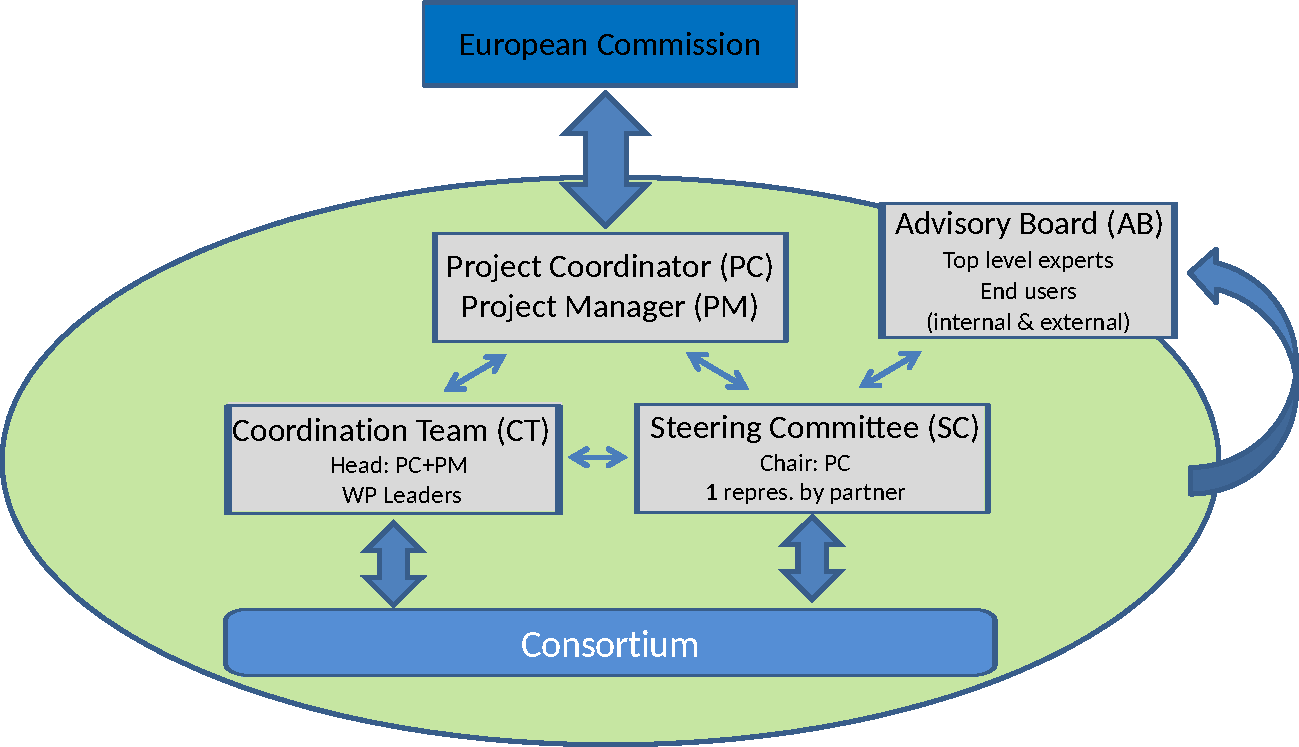
\includegraphics[width=0.75\textwidth]{management_structure.pdf}
  \caption{Management structure}
  \label{figure.management}
\end{figure}

The organisational structure, shown in the Figure~\ref{figure.management}, has been designed
to enable efficient coordination of the project --- \TODO{update}the
development and evaluation of a VRE toolkit
integrating several previously separated tools and software and
involving both academic actors and industrial stakeholders.

We have designed the management structure and procedures to deal in a
flexible manner with the following challenges:
\begin{compactitem}
\item to integrate all consortium members and to mobilise their
  expertise, knowledge and networks at every stage of the project;
\item to give the maximum attention to the end-users needs and
  requirements;
\item to continuously involve expertise and knowledge of relevant
  stakeholders and their networks, and
\item to efficiently coordinate the project implementation in a
  collaborative environment and ensure its sustainability.
\end{compactitem}

The design has been largely adapted from that of OpenDreamKit which
has proved very effective for this type of project, with some
simplification as suggested by past experience.
\begin{itemize}
\item Suppression of the Quality Review Board: its role can
  effectively be subsumed by the steering committee; also the head of
  OpenDreamKit's Quality Review Board, Hans Fanghor, will carry over
  the accumulated experience and best practices.
\item Suppression of the End User Group: as in OpenDreamKit, all
  participants are either end users themselves, or in close contact
  with such end users. To guarantee the effectiveness of this
  simplified structure, we included end users in the advisory board.
\end{itemize}


The coordinator acts as an intermediary between the Partners and
the European Commission. The coordinator will oversee the project
planning, monitor that execution is carried out in time and that
the objectives are achieved and closely interact with the project
officer for project monitoring and delivery of the performance
indicators.  The Project Manager will ensure  efficient day-to-day
management of the project, reporting, feedback to partners on
administrative, financial and legal issues, tracking of  resource
allocation and consumption, and communication inside and outside the
consortium.

The resources of all partners will be mobilised by decentralisation of
responsibilities through the assignment of leadership for work
packages. Clear distribution of tasks, efficient decision making
mechanisms and a sound financial management will safeguard the
achievement of the project's objectives.

\ifgrantagreement\else
\subsubsection{Milestones}
For a description of the milestones and their motivations see
Section~\ref{sec:milestones}; a tabulation of the milestones, which work packages
are involved, and a means of verification can be seen in Table~\ref{tab:milestonetable}.

\milestonetable
\fi

\subsubsection{Project roles}

%Project Coordinator and Project Manager can meet any time and at least
%twice a week.

The following bodies will form the organisational structure of the
\TheProject project : Coordination Team (MT), Steering Committee (SC),
Advisory Board (AB).%, End User Group (EUG) and Quality Review board (QRB).

\begin{description}
\item{\textbf{Coordination Team (CT)}} \nobreak\par
\textbf{Members:} The CT is composed of the Work Package leaders
and headed by the Project Coordinator, assisted by the Project
Manager.

\textbf{Responsibilities:} The CT is an executive body in charge of
the project implementation and monitoring.
It takes operational decisions necessary for the smooth execution of
the project.

\textbf{Tasks:}
\begin{compactenum}
\item Monitoring the timely execution of the tasks and achievement of
  the objectives;
\item Preparation of scientific and financial progress reports;
\item Controlling Work Package progress by assessing it through technical
  reports developed by the partners;
\item Making proposals to the Steering Committee of re-allocation of
  tasks, resources and financial needs for the fulfilment of the work
  plan;
\item Preparing the drafts and validating the project deliverables to
  be submitted to the Commission.
\end{compactenum}

\textbf{Meetings:} They will meet Work-Package leaders every 6 months.
If necessary, extra meetings will be arranged.

\item{\textbf{Steering Committee (SC)}}\nobreak\par

\textbf{Members:} The SC is chaired by the Project Coordinator
and includes one representative from each partner organisation.

\textbf{Responsibilities:} The SC is the decision-making body in
charge of the strategic orientation of the project.  It takes decisions on scientific
directions, re-allocation of resources, consortium
changes and intellectual property rights.

\textbf{Meetings:} Biyearly. If necessary, extra-meetings
will be arranged.  Written minutes of each meeting will be produced,
which shall be the formal record of all decisions taken. A procedure
for comment and acceptance is proposed.

\textbf{Voting procedure:} The SC shall not deliberate until a quorum
of three-fourth (3/4) of all Members are present (possibly through
video-conference) or represented. Each Member shall have one vote. The
SC will work on consensual decisions as much as possible and resort to
voting only if unavoidable. Voting decisions shall be taken by a
majority of two-thirds (2/3) of votes with quorum two-thids (2/3) of
the whole set of members. Exceptional decisions (large changes to the
budget ($\geq$ 100k euros), evolution to the consortium, firing the
coordinator, resolving ambiguity about whether something is a hard
question) shall be taken by a majority of three-fourth (3/4) of votes
with quorum three-fourth (3/4) of the whole set of members. Votes can
be electronic.

\item{\textbf{Advisory board (AB)}} \nobreak\par

  \textbf{Members:} top level experts and end-users from partner and
  external organisations, from a variety of disciplines and both from
  academic and industrial sector. Together, they have a deep
  understanding of both market and technical problems, and an
  awareness of opportunities

  \textbf{Responsibilities:} to give an independent opinion on
  steering, scientific and innovation matters, in order to guaranty
  quality implementation of the project, adequateness to the end-users
  needs, efficient innovation management, and project sustainability.

  % \textbf{Tasks:} to control the project execution from the point of
  % view of the end user needs and requirements, to test the tool and to
  % detect its potential shortcomings at the early stages, to propose
  % adaptation measures.

  \textbf{Meetings:} at the request of the Steering Committee.
\end{description}

\subsubsection{Project management tools and procedures}

Project partners and management bodies will communicate through
a dedicated project web platform, maintained by the Project
Manager. WP leaders will monitor progress of
participants of their WP at least monthly, and participants will inform their WP
leaders when problems are encountered. Major problems will be
discussed in (teleconference) meetings with the Project Coordinator
and Project Manager. Each WP leader will be free to organise
extra meetings with WP partners, if necessary. Scientific and
financial progress reports will be collected, assembled and
transmitted to the Project Coordinator by the WP leaders through the
web platform. On basis of the Progress Reports, the Coordination Team
will monitor progress of the project, identify bottlenecks and find
solutions for these problems. Where needed, adaptations to the project
plan will be made, with the aim of ensuring the delivery of the project
results as agreed with the EC. Major adaptations need to be approved
by the Steering Committee.

The Coordination Team, will ensure efficient innovation management.
They will carefully monitor new opportunities in order to suggest, if
necessary, to new directions to the Steering Committee. For legal
aspects, the latter will have a feedback from legal officers from the
Coordinator’s European Affairs and Technology Transfer office (SAIC),\TODO{Update}
specialised in Intellectual Property.

Our management structure and procedures will ensure that our network
of partners from both academic and industrial sectors is focused at
achieving the promised tasks and deliverables, efficiently managing
the innovation process and largely opening the VRE to its final users.
The partners will sign a Consortium Agreement, in which operational
rules and decision making procedures will be laid down.

\subsubsection{Risks and risk management strategy}\label{sec:risks}

The risk in the project execution as planned is carefully assessed and
managed. We base our plans on long standing experience, and we bring
together the world's experts in the relevant tools and techniques.

A key feature of this project is the involvement of a wide set of
partners from multiple domains. While this ensures complementary
coverage of a wide set of skills and provides robustness in different
ways, we will have to ensure that all partners work as closely knit
team. 

Our open source approach means that all our code and outputs
are open and visible to anybody at sites like Github and bitbucket
throughout the project. In particular, it is common for users of
computational software to use the leading edge versions, thus
beta-testing code in-between major releases. This results in risk
reduction: where our design decision or technical approaches are
controversial, this will be detected early by those users, giving the
consortium useful feedback to consider.

The project coordinator will, with support from the Coordination Team
and Quality Review Board, create a Risk Management Plan
\delivref{management}{ipr} as part of the Management Work Package,
which will be reviewed annually.
\ifgrantagreement\else
An initial risk assessment appears as figure \ref{risk-table}.

\TOWRITE{ALL}{risk about EOSC integration}

\begin{figure}
\begin{center}
\begin{tabular}{|m{.2\textwidth}|m{.12\textwidth}|m{.58\textwidth}|}\hline
  Risk & Level with/without mitigation & Mitigation measures\\\hline
  
  General technical / scientific risks\\\hline
  
  Implementing infrastructure that does not match the needs of end users & High/Low &
  Most of the members of the consortium are themselves end-users with
  a diverse range of needs and points of views; hence the design of
  the proposal and the governance of the project is naturally steered
  by demand; besides, because we provide a toolkit, users have the
  flexibility to adapt the infrastructure to their needs.\\\hline
  
  Lack of predictability for tasks that are pursued jointly with
  the community & Medium/Low &
  The PI's have a strong experience managing community-developed
  projects where the execution of tasks depends on the availability of
  partners. Some tasks may end up requiring more manpower from
  \TheProject to be completed on time, while others may be entirely
  taken care of by the community. Reallocating tasks and redefining
  work plans is common practice needed to cater for a
  fast evolving context. Such random factors will be averaged out over
  the large number of independent tasks.\\\hline
  
  Reliance on external software components & Medium/Low & The non trivial
  software components \TheProject relies on are open source. Most are
  very mature
  and supported by an active community, which offers strong long run
  guarantees.  The critical emerging software component \Jupyter
  builds on \IPython which has been around for a decade and is very
  mature. The other components could be replaced by alternatives, or
  worst comes to worst, taken over by the participants.
  \\\hline
  
  Use-case risks\\\hline
  % TO WRITE
  
  Management risks\\\hline

  Recruitment of highly qualified staff & High/Medium &
  Great care was taken identifying pool of candidates to hire from,
  and coordinating with currently running projects to rehire personnel
  with strong track record. Typically, we will rehire European
  postdocs that are currently funded by the Sloan grant to work on
  Jupyter in California and wish to come back to Europe.\\\hline

  Different groups not forming effective team & Medium/Low & Long
  track record of working collaboratively on code across multiple
  sites; Aggressive planning of project meetings, work-shops and
  one-to-one partner visits to facilitate most effective teamwork,
  combining face-to-face time at one site with remote
  collaboration.\\\hline 
  % this also justifies our generous travel budget.
  
  Partner leaves the consortium & Low/High & If the GA requires a replacement
  in order to achieve the project's objectives, the consortium will invite a new 
  relevant partner in. If a replacement is not necessary, the resources and tasks 
  of the departing partner will be reallocated to the alternative ones within the 
  consortium.\\\hline 
  
  Dissemination risks\\\hline
  
  Impact of dissemination activities is lower than planned. & Low/Medium & 
  Partners in the consortium have a proven track record of publishing in top-level 
  scientific venues with the highest impact, which reduces the risk. The Project Coordinator 
  will monitor impact of all dissemination activities. If a deficiency is identified, the consortium 
  will propose relevant corrective actions.\\\hline

  \end{tabular}
\end{center}
\caption{\label{risk-table}Initial Risk Assessment}
\end{figure}
\fi
%\TOWRITE{NT/Eugenia}{Impredictability}

%\includegraphics[width=.94\textwidth]{Pictures/Impact-img1.png}

%   But: since Open Source softwares are freely accessible, security
%   and privacy issues are a concern. Anytime a resource is shared,
%   there is greater risk of unauthorised access and contaminated data.
%   Providers must demonstrate security solutions, which should include
%   physical security controlling access to the facility and protection
%   of user data from corruption and cyber attacks.}


\TOWRITE{ALL}{
  Add a paragraph about data management plan. What data will we produce, which data is available from the start, how do we handle it...
}

%  LocalWords:  mgt Paris-Sud UPSud Thiery Sage-Combinat decentralisation textwidth hline
%  LocalWords:  textwidth Jupyter slmhnlnhfnhs hsfhs ghshsh includegraphics unauthorised

%%% Local Variables:
%%% mode: latex
%%% TeX-master: "proposal"
%%% End:
%  LocalWords:  TOWRITE subsubsection organisational compactenum ipr Impredictability
%  LocalWords:  textbf nobreak smallbreak


\draftpage
\subsection{Consortium as a Whole}
%\TO WRITE{ALL}{Proofread 3.4 consortium pass 2 [Done by Hans]}
%remove this, as we have more pressing things left.

\eucommentary{\begin{compactitem}
\item
Describe the consortium. How will it match the project's objectives?
How do the members complement one another (and cover the value chain,
where appropriate)? In what way does each of them contribute to the
project? How will they be able to work effectively together?
\item
If applicable, describe the industrial/commercial involvement in the
project to ensure exploitation of the results and explain why this is
consistent with and will help to achieve the specific measures which
are proposed for exploitation of the results of the project (see section 2.3).
\item
Other countries: If one or more of the participants requesting EU funding
is based in a country that is not automatically eligible for such funding
(entities from Member States of the EU, from Associated Countries and
from one of the countries in the exhaustive list included in General
Annex A of the work programme are automatically eligible for EU funding),
 explain why the participation of the entity in question is essential to
 carrying out the project
\end{compactitem}
}

\TheProject consortium spans the broad spectrum of actors required
for successfully developing an apt and easy-to-navigate sustainable service
accessible through the EOSC hub catering to the needs of the European
scientific community. It is composed of 4 academic institutions, 4 research
centres and 2 SMEs based in 6 different countries (Norway, France,
Netherlands, Germany, Poland, Switzerland).
The Consortium ensures a critical mass of scientific expertise and excellence
in key areas \TODO{(areas)} with RTO and SMEs of recognised
 international reputation. Namely, \TheProject consortium brings in:
\begin{compactitem}
\item A set of use cases that cover several application domains and users, and that impose very diverse
requirements on EOSC infrastructure (European XFEL, CDS ASTRO, UiO, INSERM);
\item Lead developers in the Jupyter Ecosystem, including IPython, the Jupyter Notebook, JupyterLab,
JupyterHub, Binder, MyBinder.org, Jupyter Widgets located at Simula, European XFEL, QuantStack, and
WildTreeTech,
as referenced in section \ref{jupyter-ecosystem}.
\item Experts and major promoters of the Jupyter collaborative user interfaces for interactive and exploratory
computing in a variety of scientific domains (European XFEL, QuantStack, Paris-Sud, \'Ecole Polytechnique,
Simula, Silesia, \TODO{others?}).
\item A long experience and proven track record of success with large and complex collaborative projects,
including projects focused on large-scale infrastructures and large experimental services (EGI, XFEL) as well
as experience in running large scale open source projects (Jupyter project)
\item A comprehensive range of skill sets and competencies in several relevant domains, from applied
research to standardisation to business
analysis.
\end{compactitem}

The consortium has developed through collaborations and common interests over recent years.
Some partners have been working together on different aspects of Jupyter
and software for education for many years (European XFEL, QuantStack, Simula, Wild Tree Tech),
while others joined together during a previous successful EU H2020 project OpenDreamKit (European XFEL,
Paris-Sud, Silesia, Simula).
During the course of OpenDreamKit, Paris-Sud and \'Ecole Polytechnique
ran JupyterDays events, bringing in interested members of the research community.
These community workshops led to connections with application-domain sites such as INSERM and CDS
ASTRO,
and UiO has organized similar workshops with the participation of Simula.
Ultimately, in the spirit of open science,
the partners joined together to write their proposal fully in the open on GitHub,
using the same open source collaboration tools and practices
as the Open Source Open Science community.

The project partners have been interacting through a number of
activities:

\begin{enumerate}
\item Joint software development
  \begin{itemize}
  \item Jupyter Notebook (\site{XFEL}, \site{SRL}, \site{WTT}, \site{QS})
  \item Jupyter Widgets (\site{QS}, \site{SIL}, \site{UPSUD}, \site{SRL})
  \item Binder and repo2docker (\site{SRL}, \site{WTT})
  \item thebelab (\site{QS}, \site{SRL}, \site{UPSUD})
  \item nbval (\site{XFEL}, \site{SRL})
  \item \TODO{What else?}
  \end{itemize}

\item Joint projects
  \begin{itemize}
  \item OpenDreamKit (\site{XFEL}, \site{SRL}, \site{UPSUD}, \site{SIL})
  \item PaNOSC (\site{EGI}, \site{XFEL})
  \item Computing in high school science education - iCSE4school, Erasmus+ Strategic Partnerships,
  (\site{SRL}, \site{SIL}), 2014-2017
  \item Computers in Science Education:iCSE (\site{SIL}, \site{UIO}), funded by EFS, 2011-2014.
  \item \TODO{others?}
  \end{itemize}

\item Joint publications
  \begin{itemize}
  \item \cite{Kluyver2017} (\site{XFEL}, \site{SRL}, \site{QS})
  \end{itemize}

\item Collaboration
  \begin{itemize}
  \item \TODO{Could list informal collaboration activities,
      i.e. advising each other on how to use software, binder,
      widgets. Maybe that's too detailed and too much?}

  \item MyBinder for teaching and reproducibility (\site{XFEL}, \site{SRL}, \site{WTT})
  \item Widgets for computational science (\site{XFEL}, \site{QS}, \site{SIL})
  \item OpenGATE, Monte Carlo platform for medical applications (
    \site{INSERM}, \site{UPSUD})
  \item Life Science Grid Community (\site{EGI}, \site{INSERM})
  \item JupyterDays events organised at \'Ecole Polytechnique, Paris-Sud,
  and other sites, with participation from other sites (
  \site{CDS}, \site{EP}, \site{UPSUD}, \site{SRL}).
  \item Research Bazaar workshops on Jupyter, Binder, and reproducibility
    (\site{SRL}, \site{UIO})
 \end{itemize}
\end{enumerate}

Table \ref{tab:collaboration} shows a summary of the links
between partners.

\TOWRITE{ALL}{Add previous collaborations}

% joint software/database development
% Jupyter Project software

\jointsoft{XFEL,SRL}
\jointsoft{WTT,SRL}
\jointsoft{WTT,XFEL}

% Binder
\jointsoft{SRL,WTT}

% k3d
\jointsoft{SIL,SRL}
\jointsoft{SIL,XFEL}
\jointsoft{SRL,XFEL}

% nbval
\jointsoft{XFEL,SRL}

%%s

% OpenDreamKit: UPSUD, SIL, XFEL, SRL
\jointproj{XFEL,UPSUD}
\jointproj{XFEL,SRL}
\jointproj{XFEL,SIL}

\jointproj{UPSUD,SRL}
\jointproj{UPSUD,SIL}

\jointproj{SRL,SIL}
\jointproj{UIO,SIL}

% jupyterhub deployment
\jointproj{EP,UPSUD}

% Binder persistent storage
\jointproj{UPSUD,WTT}
\jointproj{EP,WTT}

% xeus-cling
\jointsoft{QS,EP}
\jointsoft{QS,UPSUD}

% panosc
\jointproj{XFEL,EGI}

% Jupyter project publication ? XXX TIM

% Binder
\jointsoft{SRL,WTT}

% research bazaar
\jointproj{SRL,UIO}

% JupyterDays Orsay + ecole
\jointproj{UPSUD,EP}
\jointproj{UPSUD,CDS}
\jointproj{UPSUD,SRL}
\jointproj{UPSUD,QS}

\jointproj{EP,CDS}
\jointproj{EP,SRL}
\jointproj{EP,QS}

\jointproj{CDS,SRL}
\jointproj{CDS,QS}

\jointproj{SRL,QS}

% OpenGATE
\jointproj{INSERM,UPSUD}

% Life Sciences Grid
\jointproj{INSERM,EGI}

% \jointpub{A,B} % some publication

%joint supervision
% \jointsup{A,B} %

%joint organization
% \jointorga{A,B} % some org
% \jointorga{SA,UJF} % PASCO'15

% joint publications
% \jointpub{A,B} % some publication

% Jupyter publication
\jointpub{SRL,XFEL}
\jointpub{SRL,QS}
\jointpub{XFEL,QS}

\coherencetable[swsites]

%%% Local Variables:
%%% mode: latex
%%% TeX-master: "proposal"
%%% End:

%%% Local Variables:
%%% mode: latex
%%% TeX-master: "proposal"
%%% End:

\draftpage

\subsection{Resources to be Committed}\label{sec:resources}
% \begin{itemize}
\item \TOWRITE{ALL}{Check resources for your site. }
\item Compare with numbers in google docs (google docs should be
  authorative)

\item Contact Min/Hans/Katarina if the numbers in the google docs
  spreadsheet don't make sens
\item Decide how many workshops you want to run, and update resources
  accordingly.
\item If you expect to travel less than money allocate, please reduce
  your numbers - unused funds will have to be returned, and it looks
  to only request what we can use in the end.
\item Same for laptops - if you don't need one, don't request one.
  \TOWRITE{ALL}{Tick off your cell in row 161 with the date, once you
    have checked the resources for your site. }
\end{itemize}


\eucommentary{Please provide the following:
\begin{compactitem}
\item
a table showing number of person/months required (table 3.4a)
\item
a table showing 'other direct costs' (table 3.4b) for participants where
those costs exceed 15\% of the personnel costs (according to the budget
table in section 3 of the administrative proposal forms)
\end{compactitem}}

\TheProject applies for a total budget of \textbf{\euro 5,934,411.25} as the amount
required achieving the objectives. The total budget is described in the subsequent
sections together with the staff effort necessary to implement the action (Table 3.4.1).
The necessary physical resources, the quantities of each and when they would be
needed has been carefully determined on the base of the following criteria:

\begin{enumerate}

\item \textbf{Historical information} the partners involved are well experienced in the
Jupyter development, software for education, processing and scale-up; past experiences
from each partner has been taken into consideration to evaluate what, and in what
quantities, different resources will be needed in the project.
\item \textbf{Work plan structure} the deliverables and milestones identified in the project work plan.
\item \textbf{The inputs necessary to resource planning}; further, the timetable of activities has helped to identify when each resource will be needed in the project.
\item \textbf{Resource pool description} the resources available in the consortium have
been carefully analysed in order to avoid any duplicating of existing resources
and allocate efficiently and effectively the resources necessary.
\item \textbf{Cost estimating}  The approximated costs of the resources needed to
complete successfully the project activities has been estimated on the base
of: a) Resource planning results, b) Activity duration estimation (Gantt and effort form),
c) Commercially available data on durables and consumables needed,
d) Preliminary Risk Assessments.
The financial allocation among the 11 partners reflects the tasks committed by each partner
and the collaborative nature of the project itself. On the whole, the financial allocation is
well-balanced and homogeneous.
\end{enumerate}

\subsubsection{Management Level Description of Resources and Budget}
\label{sect:budget-details}

\paragraph{Staff efforts}

\eucommentary{Please indicate the number of person/months over the whole
duration of the planned work, for each work package, for each participant.
Identify the work-package leader for each WP by showing the relevant
person-month figure in bold.}

The \TheProject project is gathering sites with core
developers from the Jupyter project and history in open source
software development, and brings them together with domain specialists
from a range of domains. The major investment of the project is in
software development, which is realised through person time.

\ifgrantagreement.\else{} %
displayed in the following table.
\wpfig[label=fig:staffeffort,caption=Summary of Staff Efforts]
\fi

\paragraph{Travel, dissemination, and outreach}

The nature of this proposal -- of providing a framework that allows
design and deployment of innovative services -- means that the project
has the potential to have high impact for EOSC. At the same time, it
requires input from and engagement with a significant number of
stakeholders, including potential users of the services such as
scientists, developers of other services and other EOSC-funded
projects, other open science software projects, and the developing
EOSC itself. Consequently, requirements capture, networking, feedback,
training and education workshops and outreach activities are all
important, and the second highest cost for this project.

\subparagraph{Guidelines for travel and dissemination}
\label{sect:budget-details-travel}

We use the following guidelines for expected travel expenses:
\euro{2500} for attendance of a typical one week international
conference outside Europe (including travel, subsistence,
accommodation and registration), \euro{1250} for a corresponding
conference in Europe, \euro{750} for a one-week visit of a project
partner, for instance for coding sprints and one-to-one
research visits. We expect a similar cost per week while hosting
visitors. For the half-yearly project meetings, we expect on average a
cost of \euro{500} for travel, accommodation and subsistence.

Anticipated activities:

\begin{enumerate}
\item \emph{Project meetings}: For the 9 project meetings that take place every 6 months, we expect
the PI to attend all of them (cost of 9 * 500 = \euro{4500}). For
a researcher, we also expect that they attend all such project meetings
(\euro{4500}).

\item \emph{Hosting visitors}: We expect that the site spends \euro{2000} per year to host
external visitors contributing to the project (total \euro{8000}).

\item \emph{Site visits}: We expect the researcher to carry out 3 one-week visits to other sites
(each at \euro{750}) every year, totalling 3 * 4 * 750 = \euro{9000}
over 4 years).

\item
\emph{ Conference dissemination}: We expect the researcher to attend on average 1
international conference and 1 European meeting per year (cost of 4 *
2500 + 4 * 1250 = \euro{15000}) and the investigator to attend the
equivalent of one international or two
European gatherings (totals \euro{10000}).
\end{enumerate}

Where there are multiple investigators per site, they will share the
travel and associated costs outlined above. Where there are multiple
researchers, or researchers not employed for the full 48 months, the
travel budget is adapted accordingly.



\subparagraph{Guidelines for outreach costs}

\label{sect:budget-outreach-publication-charges}
\emph{Publication charges}: We also request \euro{3000} per partner to pay for open
access publication charges.  (Some partners have other means do pay
these costs, and for them these are not needed.)

\label{sect:budget-outreach-workshops}
\emph{Workshops}: We request funds for dissemination and outreach
activities such as workshops that facilitate community building,
provide training and disseminate best practice and encourages
sustained contributions of the community to the project and beyond the
lifetime of the funding. For a one-week workshop that we organise, we
assume a cost of 400 EUR per participant to provide a meeting
location, and subsidise accommodation and catering for attendees. A
workshop for 10 people will thus cost about \euro{4000}. Participants
donate their time and need to fund their travel from other sources. By
partially contributing to the attendance cost, we hope to enable PhD
students to engage with the project and expect positive effects on the
sustainability of the activities, by embedding the tools and knowledge
with the next generation of scientists.

Details are given in the tables below and in the work packages.

\bigskip

\noindent Some partners do not require all the costs outlined above, and have
accordingly reduced their requirements below.
\bigskip


 \subsubsection{Resource summaries for consortium member sites}
 \label{resources.summary}

 %%%%%%%%%%%%%%%%%%%%%%%%%%%%%%%%%%%%%%%%%%%%%%%%%%%%%%%%%%%%%%%%
 %
 % Guidelines for completion of partner specific resource summary:
 %
 %
 % Please explain how many person months for each person are
 % requested. Say who is the local lead. Say anything that helps to
 % understand why people are recruited as you plan, in particular if
 % this deviates from having one research for 48 months.  We can also
 % use this bit of the proposal (and the table, see below) to address
 % any other unusual arrangements.
 %
 %
 % The table should contain all non-staff costs (the EU requests that
 % this table must be present if the non-staff costs exceed
 % 15% of the total cost, but it is good practice and will show
 % openness and transparency that we show the data for all partners).
 %
 % Link back from the table to the work packages and tasks for which
 % the expenses are required. Add information that makes it easier to
 % understand why the expenses are justified.
 %
 %     To refer to a task in a work package, use "\taskref{WP-ID}{TASK-ID}" where
 %     WP-ID is the ID of the work package:
 %        WP#: WP-ID - full title
 %        ----------------------
 %        WP1: 'management' - Management
 %        WP2: 'community' - Community Building and Engagement
 %        WP3: 'component-architecture' - Component Architecture
 %        WP4: 'UI' - User interfaces
 %        WP5: 'hpc' - High Performance Computing
 %        WP6: 'dksbases' - Data/Knowledge/Software-Bases
 %        WP7: 'social-aspects' - Social Aspects
 %        WP8: 'dissem' - Dissemination
 %
 %
 %     and "TASK-ID" is the ID of the task. You can set this using
 %
 %       \begin{task}[id=TASK-ID,title=Math Search Engine,lead=JU,PM=10,lead=JU]
 %
 %     To refer to deliverables, use "\delivref{WP-ID}{DELIV-ID}" where DELIV-ID is
 %     the ID of the deliverable that can be set like this:
 %
 %       \begin{wpdeliv}[due=36,id=DELIV-ID,dissem=PU,nature=DEM]
 %           {Exploratory support for semantic-aware interactive widgets providing views on objects
 %           represented and or in databases}
 %       \end{wpdeliv}
 %
 %
 % The table is pre-populated with entries most sites are likely
 % to need. If a line does not apply to you, just delete it. If you need
 % an extra line, then add it. Use common sense: the number of rows should not
 % be very big, but at the same time it is useful to give some breakdown/explanation
 % of costs.
 %
 %
 % Eventually, try to create you entry similar in style to the others.
 % (The Southampton entry is fully populated, so use this as guidance
 % if in doubt.)
 %
 %
 %%%%%%%%%%%%%%%%%%%%%%%%%%%%%%%%%%%%%%%%%%%%%%%%%%%%%%%%%%%%%%%%

 In this section we briefly describe the requested resources. See the
 participant descriptions in the description of the consortium for the
 specific role of each member.

 %%%%%%%%%%%%%%%%%%%%%%%%%%%%%%%%%%%%%%%%%%%%%%%%%%%%%%%%%%%%%%%%%%%%%%%%%%%%%%
 \paragraph{Resources Simula Research Laboratory}

 % See line 122 in
 % https://docs.google.com/spreadsheets/d/1vXm5Z2pIWIf6UCWWkXDQ4Fti8PM6xBnpXNhehUAKmuk/edit#gid=322027044 for details
 %

 % Travel
 % Assume PI (50%) and 2 FTE researchers
 %
 % Project meetings:
 % 3 * 9000 = 27,000
 % Hosting visitors = 8000
 % Site visits 2 * 9000 = 18000
 % Conference dissemination = 2 * 15000 + 1 * 10000 = 40000
 %
 % Publication costs: 3000
 % Workshops: 4 x 10 people = 16,000
 %
 %
 %
 % Cloud computing
 % financial audit
 % laptops

 \site{SRL} requests 124 person months to provide the effort required.

 \bigskip
 \begin{table}[H]
 \begin{tabular}{|r|r|p{8.5cm}|}
   \hline
   \textbf{\site{SRL}} & \textbf{Cost (\euro)} & \textbf{Justification} \\\hline
   \textbf{Travel} &  79500 & Travel for PI and 2 researchers (see the guidelines
                              \ref{sect:budget-details-travel})\\\hline
   \textbf{Workshops} & 16000 & Workshops (40 attendees in total) (see the guidelines \ref{sect:budget-details-travel})\\\hline
   \textbf{Publication charges}
                       &  3000 & Open access publication charges (see \ref{sect:budget-outreach-publication-charges})\\\hline
 %%\textbf{Equipment}
 %%  &   0 &  \\\hline    %\taskref{WP-ID}{TASK-ID}
 \textbf{Other goods and services}
                        &  3000 & Financial audit \\\hline
   & 7500 & Consumables (3 High Performance laptops for workshops,
            sprints, dissemination )  \\\hline
 \textbf{Total}
  & 109500\\\cline{1-2}
 \end{tabular}
 \caption{Overview: Non-staff resources to be committed at Simula
   Research Laboratory
   (all in \texteuro)}\vspace*{-1em}
 \end{table}

%%  %%%%%%%%%%%%%%%%%%%%%%%%%%%%%%%%%%%%%%%%%%%%%%%%%%%%%%%%%%%%%%%%%%%%%%%%%%%%%%
%%  \paragraph{Resources Facility}
%%
%%  \site{...} requests
%%  X person months for
%%
%%  \taskref{wpid}{taskid}
%%
%%
%%  \bigskip
%%  \begin{table}[H]
%%  \begin{tabular}{|r|r|p{8.5cm}|}
%%  \hline
%%  \textbf{2: \site{SRL}} & \textbf{Cost (\euro)} & \textbf{Justification} \\\hline
%%  \textbf{Travel}
%%    &  XXX & Travel (see the guidelines \ref{sect:budget-details-travel})\\\hline
%%  \textbf{Publication charges}
%%    &   XXX & Open access publication charges (see \ref{sect:budget-outreach-publication-charges})\\\hline
%%  %%\textbf{Equipment}
%%  %%  &   0 &  \\\hline    %\taskref{WP-ID}{TASK-ID}
%%  \textbf{Other goods and services}
%%    & XXX &
%%   \\\hline   %\taskref{WP-ID}{TASK-ID} \delivref{WP-ID}{DELIV-ID}
%%  \textbf{Total}
%%   & XXX\\\cline{1-2}
%%  \end{tabular}
%%  \caption{Overview: Non-staff resources to be committed at CNRS (all in \texteuro)}\vspace*{-1em}
%%  \end{table}
%%



  %%%%%%%%%%%%%%%%%%%%%%%%%%%%%%%%%%%%%%%%%%%%%%%%%%%%%%%%%%%%%%%%%%%%%%%%%%%%%%

\paragraph{Resources CDS Astro}

\site{CDS} requests 18 person months to provide the effort required.

\bigskip
\begin{table}[H]
\begin{tabular}{|r|r|p{8.5cm}|}
  \hline
  \textbf{\site{CDS}} & \textbf{Cost (\euro)} & \textbf{Justification} \\\hline
  \textbf{Travel} &  13750 & Travel for PI and $\approx$0.4 researchers (see the guidelines
                             \ref{sect:budget-details-travel})\\\hline
  \textbf{Workshops} &  4000 & Workshop (10 attendees in total) (see the guidelines \ref{sect:budget-details-travel})\\\hline
  \textbf{Publication charges}
                      &  3000 & Open access publication charges (see \ref{sect:budget-outreach-publication-charges})\\\hline
%%\textbf{Equipment}
%%  &   0 &  \\\hline    %\taskref{WP-ID}{TASK-ID}
\textbf{Total}
 & 20750 \\\cline{1-2}
\end{tabular}
\caption{Overview: Non-staff resources to be committed at CDS (all in \texteuro)}\vspace*{-1em}
\end{table}


\paragraph{Resources \'Ecole Polytechnique}

\site{EP} requests 52 person months to provide the effort required.

\bigskip
\begin{table}[H]
\begin{tabular}{|r|r|p{8.5cm}|}
  \hline
  \textbf{\site{EP}} & \textbf{Cost (\euro)} & \textbf{Justification} \\\hline
  \textbf{Travel} &  45000 & Travel for PI and 1 researchers (see the guidelines
                             \ref{sect:budget-details-travel})\\\hline

\textbf{Workshops} & 8000 & Workshop (20 attendees in total) (see the guidelines \ref{sect:budget-details-travel})\\\hline
  \textbf{Publication charges}
                      &  3000 & Open access publication charges (see \ref{sect:budget-outreach-publication-charges})\\\hline
%%\textbf{Equipment}
%%  &   0 &  \\\hline    %\taskref{WP-ID}{TASK-ID}
  \textbf{Other goods and services}
                        &  5000 & Financial audit \\\hline
\textbf{Total}
 & 61000 \\\cline{1-2}
\end{tabular}
\caption{Overview: Non-staff resources to be committed at \'Ecole Polytechnique
  (all in \texteuro)}\vspace*{-1em}
\end{table}


\paragraph{Resources EGI}

\site{EGI} requests 24 person months to provide the effort required.

\bigskip
\begin{table}[H]
\begin{tabular}{|r|r|p{8.5cm}|}
  \hline
  \textbf{\site{EGI}} & \textbf{Cost (\euro)} & \textbf{Justification} \\\hline
  \textbf{Travel} &  20750 & Travel for PI and $\approx$0.5 researchers (see the guidelines
                             \ref{sect:budget-details-travel})\\\hline
%%\textbf{Equipment}
%% &   0 &  \\\hline    %\taskref{WP-ID}{TASK-ID}
\textbf{Other goods and services}
                      & 180000 & Cloud computing (180k) \TODO{Add location where
               this is explained; binder service}
   \\\hline   %\taskref{WP-ID}{TASK-ID} \delivref{WP-ID}{DELIV-ID}
\textbf{Total}
 & 200750 \\\cline{1-2}
\end{tabular}
\caption{Overview: Non-staff resources to be committed at EGI (all in \texteuro)}\vspace*{-1em}
\end{table}


\paragraph{Resources European XFEL}

\site{XFEL} requests 123 person months to provide the effort required.

\bigskip
\begin{table}[H]
\begin{tabular}{|r|r|p{8.5cm}|}
  \hline
  \textbf{\site{XFEL}} & \textbf{Cost (\euro)} & \textbf{Justification} \\\hline
  \textbf{Travel} &  79500 & Travel for PI and 2 researchers (see the guidelines
                             \ref{sect:budget-details-travel})\\\hline
  \textbf{Workshops} &  16000 & Workshops (40 attendees in total) (see the guidelines \ref{sect:budget-details-travel})\\\hline
  \textbf{Publication charges}
                      &  3000 & Open access publication charges (see \ref{sect:budget-outreach-publication-charges})\\\hline
%%\textbf{Equipment}
%%  &   0 &  \\\hline    %\taskref{WP-ID}{TASK-ID}
\textbf{Other goods and services}
                      &  6500 & Financial audit \\\hline
  & 7500 & Consumables (3 High Performance laptops for workshops,
           sprints, dissemination )  \\\hline
\textbf{Total}
 & 112500 \\\cline{1-2}
\end{tabular}
\caption{Overview: Non-staff resources to be committed at European XFEL (all in \texteuro)}\vspace*{-1em}
\end{table}


\paragraph{Resources INSERM}

\site{INSERM} requests 39 person months to provide the effort required.

\bigskip
\begin{table}[H]
\begin{tabular}{|r|r|p{8.5cm}|}
  \hline
  \textbf{\site{INSERM}} & \textbf{Cost (\euro)} & \textbf{Justification} \\\hline
  \textbf{Travel} &  37300 & Travel for PI and $\approx$0.8 researchers (see the guidelines
                             \ref{sect:budget-details-travel})\\\hline

\textbf{Workshops} & 4000 & Workshop (10 attendees in total) (see the guidelines \ref{sect:budget-details-travel})\\\hline
  \textbf{Publication charges}
                      &  3000 & Open access publication charges (see \ref{sect:budget-outreach-publication-charges})\\\hline
%%\textbf{Equipment}
%%  &   0 &  \\\hline    %\taskref{WP-ID}{TASK-ID}
  \textbf{Other goods and services}
%                        &  3500 & Financial audit \\\hline
  & 2500 & Consumables (1 High Performance laptop for workshops,
           sprints, dissemination)  \\\hline
\textbf{Total}
 & 46800 \\\cline{1-2}
\end{tabular}
\caption{Overview: Non-staff resources to be committed at INSERM
  (all in \texteuro)}\vspace*{-1em}
\end{table}


\paragraph{Resources QuantStack}

\site{QS} requests 48 person months to provide the effort required.

\bigskip
\begin{table}[H]
\begin{tabular}{|r|r|p{8.5cm}|}
  \hline
  \textbf{\site{QS}} & \textbf{Cost (\euro)} & \textbf{Justification} \\\hline
  \textbf{Travel} &  51000 & Travel for PI and 1 researcher (see the guidelines
                             \ref{sect:budget-details-travel})\\\hline
  \textbf{Workshops} &  8000 & Workshops (40 attendees in total) (see the guidelines \ref{sect:budget-details-travel})\\\hline
  \textbf{Publication charges}
                      &  3000 & Open access publication charges (see \ref{sect:budget-outreach-publication-charges})\\\hline
%%\textbf{Equipment}
%%  &   0 &  \\\hline    %\taskref{WP-ID}{TASK-ID}
\textbf{Other goods and services}
                      &  4000 & Financial audit \\\hline
  & 2500 & Consumables (1 High Performance laptop for workshops,
           sprints, dissemination )  \\\hline
\textbf{Total}
 & 68500 \\\cline{1-2}
\end{tabular}
\caption{Overview: Non-staff resources to be committed at QuantStack (all in \texteuro)}\vspace*{-1em}
\end{table}


\paragraph{Resources University of Oslo}

\site{UIO} requests 27 person months to provide the effort required.

\bigskip
\begin{table}[H]
\begin{tabular}{|r|r|p{8.5cm}|}
  \hline
  \textbf{\site{UIO}} & \textbf{Cost (\euro)} & \textbf{Justification} \\\hline
  \textbf{Travel} &  28060 & Travel for PI and $\approx$0.5 researchers (see the guidelines
                             \ref{sect:budget-details-travel})\\\hline

\textbf{Workshops} & 8000 & Workshop (20 attendees in total) (see the guidelines \ref{sect:budget-details-travel})\\\hline
  \textbf{Publication charges}
                      &  3000 & Open access publication charges (see \ref{sect:budget-outreach-publication-charges})\\\hline
%%\textbf{Equipment}
%%  &   0 &  \\\hline    %\taskref{WP-ID}{TASK-ID}
  \textbf{Other goods and services}
%                        &  3500 & Financial audit \\\hline
  & 2500 & Consumables (1 High Performance laptop for workshops,
           sprints, dissemination)  \\\hline
\textbf{Total}
 & 41560 \\\cline{1-2}
\end{tabular}
\caption{Overview: Non-staff resources to be committed at University
  of Oslo
  (all in \texteuro)}\vspace*{-1em}
\end{table}

\paragraph{Resources University Paris-Sud}

\site{UPSUD} requests 42 person months to provide the effort required.

\bigskip
\begin{table}[H]
\begin{tabular}{|r|r|p{8.5cm}|}
  \hline
  \textbf{\site{UPSUD}} & \textbf{Cost (\euro)} & \textbf{Justification} \\\hline
  \textbf{Travel} &  35375 & Travel for PI and $\approx$0.75 researchers (see the guidelines
                             \ref{sect:budget-details-travel})\\\hline

\textbf{Workshops} & 13500 & 2 workshops (30 attendees in total) (see the guidelines \ref{sect:budget-details-travel})\\\hline
%  \textbf{Publication charges}
%                      &  3000 & Open access publication charges (see \ref{sect:budget-outreach-publication-charges})\\\hline
%%\textbf{Equipment}
%%  &   0 &  \\\hline    %\taskref{WP-ID}{TASK-ID}
%  \textbf{Other goods and services}
%                        &  3500 & Financial audit \\\hline % Done internally for this kind of expenses at Paris-Sud
%  & 2500 & Consumables (1 High Performance laptop for workshops,
%           sprints, dissemination)  \\\hline
\textbf{Total}
 & 48875 \\\cline{1-2}
\end{tabular}
\caption{Overview: Non-staff resources to be committed at University
  Paris Sud
  (all in \texteuro)}\vspace*{-1em}
\end{table}


\paragraph{Resources University of Silesia}

\site{SIL} requests 24 person months to provide the effort required.

\bigskip
\begin{table}[H]
\begin{tabular}{|r|r|p{8.5cm}|}
  \hline
  \textbf{\site{SIL}} & \textbf{Cost (\euro)} & \textbf{Justification} \\\hline
  \textbf{Travel} &  31525 & Travel for PI and $\approx$0.65 researchers (see the guidelines
                             \ref{sect:budget-details-travel})\\\hline

%\textbf{Workshops} & 8000 & Workshop (20 attendees in total) (see the guidelines \ref{sect:budget-details-travel})\\\hline
  \textbf{Publication charges}
                      &  3000 & Open access publication charges (see \ref{sect:budget-outreach-publication-charges})\\\hline
%%\textbf{Equipment}
%%  &   0 &  \\\hline    %\taskref{WP-ID}{TASK-ID}
  \textbf{Other goods and services}
%                        &  3500 & Financial audit \\\hline
                       &  \TODO{total} & Contracted development \\\hline
  & 2500 & Consumables (1 High Performance laptop for workshops,
           sprints, dissemination)  \\\hline
\textbf{Total}
 & 37025 \\\cline{1-2}
\end{tabular}
\caption{Overview: Non-staff resources to be committed at University of Silesia
  (all in \texteuro)}\vspace*{-1em}
\end{table}


\paragraph{Resources Wild Tree Tech}

\site{WTT} requests 36 person months to provide the effort required.

\bigskip
\begin{table}[H]
\begin{tabular}{|r|r|p{8.5cm}|}
  \hline
  \textbf{\site{WTT}} & \textbf{Cost (\euro)} & \textbf{Justification} \\\hline
  \textbf{Travel} &  36145 & Travel for PI and $\approx$0.75 researchers (see the guidelines
                             \ref{sect:budget-details-travel})\\\hline

%%\textbf{Equipment}
%%  &   0 &  \\\hline    %\taskref{WP-ID}{TASK-ID}
  \textbf{Other goods and services}
                        &  4000 & Financial audit \\\hline
  & 2500 & Consumables (1 High Performance laptop for workshops,
           sprints, dissemination)  \\\hline
\textbf{Total}
 & 42645 \\\cline{1-2}
\end{tabular}
\caption{Overview: Non-staff resources to be committed at Wild Tree Tech
  (all in \texteuro)}\vspace*{-1em}
\end{table}


% ---------------------------------------------------------------------------
%  Section 4: Members of the Consortium
% ---------------------------------------------------------------------------

\newpage

\eucommentary{This section is not covered by the page limit.\\
The information provided here will be used to judge the operational capacity.}

\section{Members of the Consortium}
\TOWRITE{ALL}{Proofread 4. Members of the consortium pass 2}

\subsection{Participants}

\eucommentary{Please provide, for each participant, the following (if available):\\
\begin{compactitem}
\item
a description of the legal entity and its main tasks,
with an explanation of how its profile matches the tasks in the proposal;
\item
a curriculum vitae or description of the profile of the persons,
including their gender, who will be primarily responsible for carrying
out the proposed research and/or innovation activities;
%
this includes a description of the profile of the to-be-recruited personnel
\item
a list of up to 5 relevant publications, and/or products, services
(including widely-used datasets or software), or other achievements
relevant to the call content;
\item
a list of up to 5 relevant previous projects or activities, connected
to the subject of this proposal;
\item
a description of any significant infrastructure and/or any major items
of technical equipment, relevant to the proposed work;
\item
any other supporting documents specified in the work programme for this call.
\end{compactitem}}

\begin{sitedescription}{SRL}

Dedicated to tackling scientific challenges with long-term impact and of genuine importance to real life, Simula Research Laboratory (Simula) offers an environment that emphasises and promotes basic research. At the same time, we are deeply involved in research education and application-driven innovation and commercialisation.

Simula was established as a non-profit, limited company in 2001, and is fully owned by the Norwegian Ministry of Education and Research. Its research is funded through competitive grants from national funding agencies and the EC, research contracts with industry, and a basic allowance from the state.  Simula's operations are conducted in a seamless integration with the two subsidiaries Simula School of Research and Innovation and Simula Innovation.

At its outset, the laboratory was given the mandate of becoming an internationally leading research institution within select fields in information and communications technology. These fields are (i) communication systems, including cyber-security; (ii) scientific computing, aiming at fast and reliable solutions of mathematical models in biomedicine, geoscience, and renewable energy; and (iii) software engineering, focusing on testing and verification of mission-critical software systems, and on planning and cost estimation of large software development projects. Recent evaluations state that Simula has met its challenge and is an acknowledged contributor to top-level research in its focus areas. Specifically, in the 2012 national evaluation of ICT research organised by the Research Council of Norway and conducted by an international expert panel, Simula received the highest average score (4.67) on a 1-5 scale among all evaluated institutions.  In comparison, the national average was 3.38. Only five of the 62 research groups evaluated were awarded the top grade (5), and two of these five groups are located at Simula.

Simula is currently hosting one Norwegian Centre of Excellence, Centre for Biomedical Computing (2007-2017), and one Norwegian Centre for Research-based Innovation, Certus (2011-2018). In addition, we participate as research partner in another Centre for Research-based Innovation, Centre for Cardiological Innovation (2011-2018), hosted by Oslo University Hospital. These two centre-oriented schemes are the most prestigious funding instruments offered by the Research Council of Norway.

\subsubsection*{Curriculum vitae}

% Curriculum of the personnel at this institution

% \input{CVs/Martin.Sandve.Alnaes.tex}
% \input{CVs/Simula-not-known.tex}
% \input{CVs/First.Last.tex}

\subsubsection*{Publications, products, achievements}

\begin{compactenum}
\item Jupyter, ...
\end{compactenum}

\subsubsection*{Previous projects or activities}

\begin{compactenum}
\item OpenDreamKit
\item Jupyter
\item Binder
\end{compactenum}

\subsubsection*{Significant infrastructure}

The fully owned Simula subsidiary Simula Innovation handles pre-commercial innovation projects, creation and follow-up of company spin-offs, and general support for entrepreneurs.
\end{sitedescription}



%KEY-MORE-TODOS


%%% Local Variables:
%%% mode: latex
%%% TeX-master: "../proposal"
%%% End:

%  LocalWords:  sitedescription Simula Simula commercialisation Certus subsubsection Logg
%  LocalWords:  Mardal Funke Rognes Sci Comput Langtangen FEniCS Aln ae lgaard vspace
%  LocalWords:  TOWRITE emphasises organised

\clearpage
\begin{sitedescription}{XFEL}
  \label{sitedescription:euxfel}

% PIC:
% see: http://ec.europa.eu/research/participants/portal/desktop/en/orga

% See ../proposal.tex, section Members of the Consortium for a
% complete description of what should go there

  European X-Ray Free-Electron Laser Facility GmbH is a limited
  liability company under German law. At present, 12 countries are
  participating in the project: Denmark, France, Germany, Hungary,
  Italy, Poland, Russia, Slovakia, Spain, Sweden, Switzerland, and the
  United Kingdom.  The company is in charge of the operation and
  construction of the European XFEL, a 3.4 km long X-ray free-electron
  laser facility extending from Hamburg to the neighbouring town of
  Schenefeld in the German federal state of Schleswig-Holstein. Civil
  construction started in early 2009, and the user operation in
  September 2017. With its repetition rate of 27,000 pulses per second
  and a peak brilliance a billion times higher than that of the best
  synchrotron X-ray radiation sources, the European XFEL will allow
  the investigation of still open scientific problems in a variety of
  disciplines (physics, structural biology, chemistry, planetary
  science, study of matter under extreme conditions and many others).

  European XFEL has a data policy in place \cite{datapolicy-euxfel}
  which opens up facility data for open access after an embargo period
  of 3 years.
\subsubsection*{Curriculum vitae}

% Curriculum of the personnel at this institution
%
\begin{participant}[type=leadPI,PM=4,gender=male]{Hans Fangohr}
  % type is one of:
  % - leadPI: leader of the participating institution
  % - PI: Principal Investigator
  % - R: researcher?
  % Who is the coordinator is specified elsewhere

  % PM=YYY:
  % A fair evaluation of the number of months you will be
  % spending on this specific project along the four years.
  % Typical numbers:
  % - full time hired personnel: 48 months
  % - lead PI or proposal coordinator: 8-12 months
  % - PI: 4-5 months
  % - participant: 2-6 months

  % salary=ZZZ:
  % Approximate monthly gross salary (in term of total cost for the
  % employer). This is optional. If you are uncomfortable having this
  % information in a public file, you can alternatively send the
  % information to Eugenia Shadlova, or to your institution
  % leader/manager if he is willing to fill in himself the budget
  % forms on the eu portal.

  % The above information is used to fill in various tables in the
  % proposal file, and to evaluate the cost of the project for the
  % institutions.

  % You may remove all those comments.

  % About half a page of free text; for whatever it's worth, you may see
  % Nicolas.Thiery.tex for an example.



  \medskip Hans Fangohr is an academic at the University
  of Southampton in the United Kingdom since 2002 (full professor
  since 2010), and leading the data analysis services at European XFEL
  in Germany since 2017.

  He has been a long term proponent of Open Science, and in particular
  involved with the the use and further development of the Jupyter
  Notebook to enable this. He has hosted Thomas Kluyver at the
  University of Southampton since 2015 from where he contributed as a
  core developer of the Jupyter team. As a PI in the EC-funded e-INFRA
  OpenDreamKit project (2015-2019), he has pushed forward the use of
  Jupyter Notebooks for reproducible computational science, and
  started the notebook validation tool (NBVAL). He made use of the
  Jupyter Ecosystem for research and education at graduate and
  postgraduate level at the University of Southampton, and shared
  resources widely, including a text book provided through Jupyter
  Notebooks, which can be executed interactively online [1].

  Since 2017, he is designing data analysis services and
  infrastructure at the European XFEL research facility. European XFEL
  is using IPython and the Jupyter Notebook as core utilities in their
  large scale experiment control, data capture and data
  analysis. Within the e-INFRA project PaNOSC (Photon and Neutron
  Science Open Cloud, 2019-2022), he is leader of the Work Package 4,
  which is focused on data analysis services for the EOSC Hub, and the
  use of the Jupyter notebook with its existing features on the EOSC
  hub.

  In this project (BOSSEE), where new capabilities for the Jupyter
  notebook and ecosystem are being designed, Hans' wide experience and
  interaction with different science groups will be beneficial to
  ensure the outcome is of value to open science in many domains. This
  includes him chairing the interdisciplinary computational modelling
  group at the University of Southampton (200 academics, 2008-2017),
  chairing the national EPSRC scientific advisory committee on High
  Performance Computing in the UK (2014-2017) and interacting with a
  large variety of science users at European XFEL in his current role
  to support their data analysis.
\end{participant}

%%% Local Variables:
%%% mode: latex
%%% TeX-master: "../proposal"
%%% End:

\begin{participant}[type=PI,PM=1,gender=male]{Sandor Brockhauser}
  % type is one of:
  % - leadPI: leader of the participating institution
  % - PI: Principal Investigator
  % - R: researcher?
  % Who is the coordinator is specified elsewhere

  % PM=YYY:
  % A fair evaluation of the number of months you will be
  % spending on this specific project along the four years.
  % Typical numbers:
  % - full time hired personnel: 48 months
  % - lead PI or proposal coordinator: 8-12 months
  % - PI: 4-5 months
  % - participant: 2-6 months

  % salary=ZZZ:
  % Approximate monthly gross salary (in term of total cost for the
  % employer). This is optional. If you are uncomfortable having this
  % information in a public file, you can alternatively send the
  % information to Eugenia Shadlova, or to your institution
  % leader/manager if he is willing to fill in himself the budget
  % forms on the eu portal.

  % The above information is used to fill in various tables in the
  % proposal file, and to evaluate the cost of the project for the
  % institutions.

  % You may remove all those comments.

  % About half a page of free text; for whatever it's worth, you may see
  % Nicolas.Thiery.tex for an example.


  \medskip

  Sandor Brockhauser is the head of the Control and Analysis Software
  Group at the European XFEL. He received his M.Sc. in Informatics
  from Technical University of Budapest, Hungary, earned a Ph.D. from
  University of Leoben, Austria, and received his HDR degree in
  physics at the University of Joseph Fourier, Grenoble in
  France.

  Since 2004, when he joined the European Molecular Biology
  Laboratory (EMBL) in Grenoble, France, he worked in Macromolecular
  Crystallography and became the scientist in charge of the Multi-
  Wavelength Anomalous Dispersion Beamline ID14-4 at European
  Synchrotron Radiation Facility (ESRF), France. Between 2013-15, he
  moved to Szeged, Hungary where he joined the Extreme Light
  Infrastructure, ELI-ALPS, and has established and built up its
  Scientific Engineering Division. In the same time, he also
  established the X-ray Crystallography Laboratory at a European
  Center of Excellence, the Biological Research Center, Szeged of the
  Hungarian Academy of Sciences. Moving to the European XFEL in 2016,
  he became responsible for the full control system of the beamlines
  and scientific instruments, Karabo, that enables the integration of
  Experiment Control, Data Acquisition and Analysis. During the last
  two years, Karabo has been deployed, photon beamlines were
  successfully commissioned and two of the initial scientific
  instruments have been put in operation producing 0,5PT of data in 5
  weeks of experiments. Jupyter tools are embedded in the Karabo
  system and European XFEL analysis activities.

\end{participant}

%%% Local Variables:
%%% mode: latex
%%% TeX-master: "../proposal"
%%% End:

\begin{participant}[type=leadPI,PM=1,gender=male]{Krzysztof Wrona}
  % type is one of:
  % - leadPI: leader of the participating institution
  % - PI: Principal Investigator
  % - R: researcher?
  % Who is the coordinator is specified elsewhere

  % PM=YYY:
  % A fair evaluation of the number of months you will be
  % spending on this specific project along the four years.
  % Typical numbers:
  % - full time hired personnel: 48 months
  % - lead PI or proposal coordinator: 8-12 months
  % - PI: 4-5 months
  % - participant: 2-6 months

  % salary=ZZZ:
  % Approximate monthly gross salary (in term of total cost for the
  % employer). This is optional. If you are uncomfortable having this
  % information in a public file, you can alternatively send the
  % information to Eugenia Shadlova, or to your institution
  % leader/manager if he is willing to fill in himself the budget
  % forms on the eu portal.

  % The above information is used to fill in various tables in the
  % proposal file, and to evaluate the cost of the project for the
  % institutions.

  % You may remove all those comments.

  % About half a page of free text; for whatever it's worth, you may see
  % Nicolas.Thiery.tex for an example.



  \medskip Krzysztof Wrona has a background in computer physics. As
  the group leader of IT and Data Management at European XFEL, he is
  in charge of the management of scientific data in the frame of the
  user program of the European XFEL facility. He has more than 15
  years of experience in data storage, processing, and in general IT
  issues.
\end{participant}

%%% Local Variables:
%%% mode: latex
%%% TeX-master: "../proposal"
%%% End:

\begin{participant}[type=R,PM=1,gender=male]{Thomas Kluyver}
  % PM=YYY:
  % A fair evaluation of the number of months you will be
  % spending on this specific project along the four years.
  % Typical numbers:
  % - full time hired personnel: 48 months
  % - lead PI or proposal coordinator: 8-12 months
  % - PI: 4-5 months
  % - participant: 2-6 months

  % salary=ZZZ:
  % Approximate monthly gross salary (in term of total cost for the
  % employer). This is optional. If you are uncomfortable having this
  % information in a public file, you can alternatively send the
  % information to Eugenia Shadlova, or to your institution
  % leader/manager if he is willing to fill in himself the budget
  % forms on the eu portal.
  Thomas Kluyver is one of the core maintainers of the Jupyter and IPython
  projects, which form a central part of this proposal.
  He has been a contributor to these projects since 2011,
  and is closely familiar with key parts of the code.
  Besides Jupyter, Thomas has contributed to a wide range of open source
  software projects in the Python ecosystem, ranging from other scientific
  computing tools such as h5py to packaging utilities such as Flit, as well
  as improvements in the Python standard library.
  
  Thomas is part of the Data Analysis team at European XFEL.
  He has a specific remit to facilitate the use of Jupyter by internal groups
  and visiting researchers,
  but he also contributes to the general software engineering effort working to
  allow convenient, reproducible analysis of data collected at European XFEL.

  Before working as a software engineer, Thomas studied plant biology, gaining
  a PhD from the University of Sheffield in 2013. His work since then has
  continued in close connection with research, at the University of California,
  Berkeley, and the University of Southampton, before joining European XFEL.
\end{participant}

%%% Local Variables:
%%% mode: latex
%%% TeX-master: "../proposal"
%%% End:

%


\begin{participant}[PM=68, type=R]{Research Engineer x2}

We will hire two postdoctoral-level research software engineers (for 68 person
months in total) to carry out the required work for this projet at
European XFEL. They will work under supervision of Hans Fangohr, with
support from Sandor Brockhauser and Krzysztof Wrona for particular
aspects. The employees will either have a scientific background and
significant software engineering expertise, or an education in
computer science and an aptitude to work with scientists on
computational science and data science problems.
\end{participant}

\subsubsection*{Publications, products, achievements}

\begin{compactenum}
\item H.Fangohr, Python for Computational Science and Engineering
  (2018) DOI: 10.5281/zenodo.1411868 \newline
  https://github.com/fangohr/introduction-to-python-for-computational-science-and-engineering
\item H.Fangohr et al., “Data Analysis support in Karabo at European
  XFEL”, Proceedings of International Conference on Accelerator and
  Large Experimental Physics Control Systems 2017, ISBN 978-3-95450-
  193-9, Data Analytics, Barcelona, Spain, TUCPA01 (2017) DOI: 10.18429/JACoW-ICALEPCS2017-TUCPA01
\item H.Fangohr.
\emph{A Comparison of \software{C}, \Matlab and \Python as Teaching Languages in Engineering}
Lecture Notes on Computational Science \textbf{3039}, 1210-1217 (2004)
\item T. Kluyver, B. Ragan-Kelley, F. Perez, B. Granger, M. Bussonier, J. Frederic, K. Kelley, J. Hamrick, J. Grout, S. Corlay et al. Jupyter
\emph{Notebooks: a publishing format for reproducible computational workflows} In 20th International Conference on Electronic Publishing. IOS Press, 2016.
\end{compactenum}

\subsubsection*{Relevant projects or activities}

\begin{compactenum}
\item OpenDreamKit (GA No. 676541) Open Digital Research Environment
  Toolkit for the Advancement of Mathematics, participant
\item EOSCpilot (GA No. 739563) The European Open Science Cloud for
  Research Pilot Project, participant
\item PaNOSC (GA No. 823852) Photon and Neutron Open Science Cloud,
  participant
\item CALIPSOplus (GA No. 730872) Convenient Access to Light Sources
  Open to Innovation, Science and to the World, participant
\item ATTRACT (GA No. 777222) breAkThrough innovaTion pRogrAmme for a
  pan-European Detection and Imaging eCosysTem, participant

\end{compactenum}




\end{sitedescription}



%KEY-MORE-TODOS



%%% Local Variables:
%%% mode: latex
%%% TeX-master: "../proposal"
%%% End:

%  LocalWords:  sitedescription Programme organisations programmes Centres subsubsection
%  LocalWords:  micromagnetic Nmag Fischbacher Franchin Bordignon Fangohr emph textbf
%  LocalWords:  Multiphysics summarised Iridis TFlops Modelling

\clearpage
\begin{sitedescription}{UPSUD} \label{desc:ParisSud}

Université Paris-Sud is among the 40 top universities worldwide in the
2013 Shanghai ranking, and is one of the top two French research
universities. With about 27000 students, 1800 permanent faculty
and 1300 permanent research scientists from national research
organisations (CNRS, Inserm, INRA, Inria), it is the largest campus in
France. Since 2006, scientists from the University were awarded two
Fields medals, one Nobel Prize and a number of other national and international prizes
(European Inventor Award 2013, Wolf Prize 2010, Holweck Prize 2009,
Japan prize 2007).  Université Paris-Sud offers a
wide range of qualifications, from the exact sciences to life and health
sciences (including medical practice), legal sciences and economics. 
Research at Université Paris-Sud is an essential part of academic understanding 
and includes research activities with high commercial potential. 
Research contracts and partnership with companies make
Université Paris-Sud a key actor and a major player in French
research.  The University is located partly on the Plateau de Saclay,
the largest cluster of public and private R\&D institutions in France
(with ca. 16000 research staff), and is one of the core members of 
University Paris-Saclay – a world-class university and a
world-renowned research and innovation hub.

In the context of this project, Université Paris-Sud is the
home of one of the largest group of \Sage developers worldwide.
It is a member of the Open Source Thematic Group of the Systematic
Paris Region Systems and ICT Cluster. 
The University also hosts a major research group in Human-Centered Computing
and manages the Digiscope network of high-end visualisation platforms,
which will provide critical assets to the project.

\subsubsection*{Curriculum vitae of the investigators}

\begin{participant}[type=PI,PM=1,gender=male]{Michel Beaudouin-Lafon}

Michel Beaudouin-Lafon (PhD, Université Paris-Sud) is a Professor of Computer Science, classe exceptionnelle, 
at Université Paris-Sud and a senior fellow of Institut Universitaire de France. 
His research interests include fundamental aspects of interaction, novel interaction techniques, 
computer-supported cooperative work and engineering of interactive systems. 
He has published over 180 papers and is a member of the ACM SIGCHI Academy. 
He is the laureate of an ERC Advanced Grant exploring instrumental interaction and information substrates. 
Michel was director of LRI, the laboratory for computer science joint between Université Paris-Sud and CNRS. 
He now heads the Human-Centered Computing lab at LRI and chairs the Computer Science department at Université Paris-Saclay. 
He was Technical Program Co-chair for CHI 2013 (3500 participants), sits on the editorial boards of ACM Books and ACM TOCHI, 
and has served on many ACM committees. He received the ACM SIGCHI Lifetime Service Award in 2015.

\end{participant}

%%% Local Variables:
%%% mode: latex
%%% TeX-master: "../proposal"
%%% End:

\begin{participant}[type=PI,PM=2,gender=female]{Viviane Pons}
  Maître de Conférences at the Laboratoire de Recherche en Informatique, Viviane Pons is a
  young researcher in Algebraic Combinatorics. She defended her thesis in 2013 and has 4
  papers in international journals and 5 communications in international
  conferences, including a talk at PyCon US 2015. 
  She also is in the editorial board of the Journal of Open Source Software.
  Before starting her research career,
  she worked for two years in industry as a Java and web developer.

  She discovered \Sage during her first \Sage Days in 2010 and has since been an active user
  and contributor with 10 (co)authored tickets improving the support of combinatorial
  objects in \Sage. She is heavily involved in the promotion of \Sage, participating in
  \Sage Days and running \Sage introduction tutorials or \Sage presentations at various
  conferences. She is also one of the main developers of the project \software{FindStat}
  dedicated to databases in combinatorics.

  Viviane is leading the very successful Community Building and
  Dissemination work package of the European Research Infrastructures
  project OpenDreamKit (2015-2019), in which 66 events (development
  workshops, training sessions, ...) were organized or coorganized,
  with more than a thousand trainees. Viviane herself organized or
  coorganized several of them, including two week-long workshops
  dedicated to women.
\end{participant}
%%% Local Variables:
%%% mode: latex
%%% TeX-master: "../proposal"
%%% End:

\begin{participant}[type=leadPI,PM=5,gender=male]{Nicolas M. Thiéry}
  Professor at the Laboratoire de Recherche en Informatique, Nicolas M. Thiéry is a senior
  researcher in Algebraic Combinatorics with 18 papers published in international
  journals. Among other things, he is a member of the permanent committee of FPSAC, the
  main international conference of the domain, and has collaborators
  in the US and Canada where he cumulatively spent more than three
  years (Colorado School of Mines, UC Davis, Providence, Montréal),
  and India. He also
  co-organised fourteen international workshops, in particular \Sage Days, and the semester
  long program on ``Automorphic Forms, Combinatorial Representation Theory and Multiple
  Dirichlet Series'' hosted in Providence (RI, USA) by the Institute for Computational and
  Experimental Research in Mathematics.

  Algebraic combinatorics is a field at the frontier between mathematics and computer
  science, with heavy needs for computer exploration. Pioneer in community-developed open
  source software for research in this field, Thiéry founded in 2000 the \SageCombinat
  software project (incarnated as \MuPADCombinat until 2008); with 50 researchers
  in Europe and abroad, this project has grown under
  his leadership to be one of the largest organised community of Sage developers, gaining
  a leading position in its field, and making a major impact on one hundred
  publications\footnote{\url{http://sagemath.org/library-publications-combinat.html},
    \url{http://sagemath.org/library-publications-mupad.html}}. Along the way,
%this occasion
%Thiéry gained a strong community building experience, and
  he coauthored part of the proposal for NSF \SageCombinat grant
  OCI-1147247, and co-organised or taught at a dozen training and
  dissemination actions (workshops, summer schools, etc.), in
  America, Africa, Europe, and India.

  With 150 tickets (co)authored and as many refereed, Thiéry is himself a core \Sage
  developer, with contributions including key components of the \Sage infrastructure
  (e.g. categories), specialised research libraries (e.g. root systems), thematic
  tutorials, and two chapters of the book ``Calcul Mathématique avec \Sage''
  and its English translation.

  Based on this experience, and to tackle the pressing funding needs
  in the ecosystem of open source mathematical software, Thiéry
  initiated and lead the European Research Infrastructures project
  OpenDreamKit \#676541 (2015-2019, 15 sites, 50 participants, 8M€),
  engaging the Jupyter project on board. This in turn increased his
  involvement in using, promoting, and contributing to Jupyter, for
  use in mathematics and education.
\end{participant}
%%% Local Variables:
%%% mode: latex
%%% TeX-master: "../proposal"
%%% End:


\begin{participant}[type=res,PM=18]{NN}
  We will hire a full time experienced software developer to work on
  task~\taskref{math-widgets} and~\taskref{helpdesk} %longtaskref
  under the leadership of Nicolas M. Thiéry.

  The fellow will have a strong software engineering and web
  development experience, ideally in the Python, Javascript, and/or
  Jupyter ecosystem. We further require good communication and team
  working skills, in particular to work in tight collaboration with
  international open-source developer communities.
\end{participant}

\begin{participant}[type=res,PM=12]{NN}
  We will hire a full time experienced software developer to work
  on task~\taskref{collaboration} %longtaskref
  under the leadership of Michel Beaudouin-Lafon.

  The fellow will have a strong software engineering and web
  development experience (HTML/CSS/Javascript), and ideally 
  good knowledge of the Python/Jupyter ecosystems
  and/or collaboration technologies. 
  We further require good communication and team
  working skills, in particular to work in tight collaboration with
  international open-source developer communities.
\end{participant}

% Participation:
% NT: Project Management: 4PM, Component Architecture: 4PM,
%     Training/Dissemination: 2PM, User Interfaces: 2PM
% Dev 1: Component Architecture: 48PM
% Dev 2: User Interface: 24PM, CA: 10PM, HPC: 2PM
% Florent: HPC: 4PM, User Interface: 2PM (Sphinx & co)
% Viviane: Training/Dissemination: 6PM
% Loic: Training/Dissemination: 3PM, User Interfaces: 2PM
% Sam: Training/Dissemination: 6PM
% Project manager: Project management: 24PM
% PHD: ???
% Total:

\subsubsection*{Publications, achievements}

\begin{compactenum}
\item Leadership of the \SageCombinat software project.
\item Coauthoring of the open source book ``Calcul Mathématique avec
  Sage'' and its English translation , the first of its kind
  comprehensive introduction to computational mathematics in \Sage for
  education.
\item Contribution of more than 500 tickets to \Sage.
\item
Michel Beaudouin-Lafon, Olivier Chapuis, James Eagan, Tony Gjerlufsen, Stéphane Huot, Clemens Klokmose, Wendy Mackay, Mathieu Nancel, Emmanuel Pietriga, Clément Pillias, Romain Primet, Julie Wagner (2012). Multi-surface Interaction in the WILD Room, \emph{IEEE Computer}, 45(4):48–56. IEEE Computer Society.
\item
Klokmose, C.N., Eagan J.R., Baader, S., Mackay, M. and Beaudouin-Lafon, M. (2015) Webstrates: Shareable Dynamic Media. In \emph{Proceedings of the 28th annual ACM symposium on User interface software and technology (UIST ’15)}. ACM.
\end{compactenum}

\subsubsection*{Relevant projects or activities}

\begin{compactenum}
\item OpenDreamKit (GA No. 676541) Open Digital Research Environment
  Toolkit for the Advancement of Mathematics, \textbf{coordination}.
\item Hosting or coorganisation of dozens of Sage Days (week-long training and development workshops).
\item \TODO{This is not a ``previous'' project''}
Ongoing ERC Advanced Grant ONE ``Unified Principles of Interaction'' (PI: Michel Beaudouin-Lafon) that develops new user interface concepts, in particular for multi-user, multi-device environments.
\end{compactenum}

\subsubsection*{Significant infrastructure}

\site{UPSUD} hosts a local OpenStack based cloud infrastructure
\software{Cloud@VD} (400 cores) for its personnel. The participants
are regular users of this infrastructure, and in close contact with
its maintainers. As a continuation of the existing deployment of a
JupyterHub service on this infrastructure, \software{Cloud@VD} will be
available to the participants as test bed for deploying Jupyter based
services (see e.g. \taskref{eosc}{jh-bh-deployment}).

\site{UPSUD} also manages the Digiscope (\url{http://digiscope.fr}) network of high-end visualisation platforms and hosts the \software{WILD} and \software{WILDER} platforms, two ultra-high resolution wall-sized displays with motion capture and touch input for conducting research on collaborative human-computer interaction and visualisation of
large datasets.

\end{sitedescription}



\begin{draft}
\vspace{1cm}\TOWRITE{VP}{Complete check list below -- delete completed items if you wish}

\begin{verbatim}
- [ ] checked that sum of person months put into finance request is
  the same as sum of person months associated with the Work Packages
  (in proposal.tex, as defined as part of the \begin{workpackage}"
  command.

  Take into account person months associated with work package 1, time
  of all staff to be hired and work on the project (including
  investigators). Figure 5 helps with a quick check of the sums over
  different work packages.

- [X] completed site specific resource summary in resources.tex,
  including table of non-staff costs. This is compulsory (EU
  regulations) if the non-staff cost exceed 15% of the total cost, and
  is likely to be the case for most of the partners. We ask everybody
  to do it, to be consistent and show transparently how we have
  planned our total budget.

- [X] Have all our tasks a designated lead institution? Check in the
  Work Packages that all the tasks you are involved in have a
  dedicated lead party. If the lead party is "USO", then use:
  \begin{task}[lead=USO]

- [ ] Have all our deliverables a designated lead institution [using
  the 'lead=' key]?

- [X] In the "Members of the consortium section", have we addressed "a
  description of the legal entity and its main tasks, with an
  explanation of how its profile matches the tasks in the
  proposal"? See Entry for Paris-Sud and Southampton as examples.

- [X] In the Members of the consortium section, have we given
  descriptions of all the people we intend to hire (even if we don't
  know who that is yet).

- [ ] Do all our tasks include us in the list of sites involved?
\end{verbatim}
\end{draft}

%KEY-MORE-TODOS


%%% Local Variables:
%%% mode: latex
%%% TeX-master: "../proposal"
%%% End:

%  LocalWords:  sitedescription Paris-Sud organisations Inserm Inria Holweck valorisation
%  LocalWords:  Saclay subsubsection faut formel des projets antérieurs Acronyme titre
%  LocalWords:  agence financement durée Pareil les publi année SageCombinat Calcul avec
%  LocalWords:  Mathématique Logilab Sud texttt Stratuslab Chapuis

\clearpage
\begin{sitedescription}{QS}

\par QuantStack was founded in 2016 by a team of developers and maintainers of key packages of the open-source scientific computing stack. QuantStack provides support and custom development services in the Jupyter and Scientific Python ecosystems. Clients and partners of QuantStack range from financial software companies to robotics startups and public research institutions. The team comprises several core developers of Jupyter subprojects and authors of popular scientific computing and visualization software used in both academic and industrial contexts.

\par Beyond Project Jupyter, projects developed at QuantStack include data visualization packages for Jupyter such as bqplot, ipyvolume, ipyleaflet, and ipysheet, as well as Jupyter language kernels such as xeus-cling and xeus-python, and JupyterLab extensions like te draw.io and sidecar. QuantStack is also behind the development of the xtensor framework, a high-level array computing library and C++ dataframe.

\subsubsection*{Curriculum vitae of the investigators}

\begin{participant}[type=leadPI,PM=6,gender=male]{Sylvain Corlay}
  % PM=YYY:
  % A fair evaluation of the number of months you will be
  % spending on this specific project along the four years.
  % Typical numbers:
  % - full time hired personnel: 48 months
  % - lead PI or proposal coordinator: 8-12 months
  % - PI: 4-5 months
  % - participant: 2-6 months

  % salary=ZZZ:
  % Approximate monthly gross salary (in term of total cost for the
  % employer). This is optional. If you are uncomfortable having this
  % information in a public file, you can alternatively send the
  % information to Eugenia Shadlova, or to your institution
  % leader/manager if he is willing to fill in himself the budget
  % forms on the eu portal.
  Sylvain Corlay is the founder and CEO of QuantStack. He holds a PhD in applied mathematics from University Paris VI.

  As an open source developer, Sylvain contributes to Project Jupyter in the area of interactive widgets for the notebook, and is steering committee member of the Project. He also serves as a member of the board of directors for the NumFOCUS foundation, and co-organizes the PyData Paris Meetup, a regular seminar series on open-source scientific computing.

  Sylvain was one of the 15 core Jupyter developers to receive the 2017 ACM Software System Award.

  Besides Jupyter, Sylvain authors and contributes to a number of scientific computing open-source projects such as bqplot, xtensor and ipyleaflet.

  Prior to founding QuantStack, Sylvain was a quant researcher at Bloomberg and an adjunct faculty member at the Courant Institute and Columbia University.
\end{participant}

%%% Local Variables:
%%% mode: latex
%%% TeX-master: "../proposal"
%%% End:

\begin{participant}[type=R,PM=0,gender=male]{Johan Mabille}
  % PM=YYY:
  % A fair evaluation of the number of months you will be
  % spending on this specific project along the four years.
  % Typical numbers:
  % - full time hired personnel: 48 months
  % - lead PI or proposal coordinator: 8-12 months
  % - PI: 4-5 months
  % - participant: 2-6 months

  % salary=ZZZ:
  % Approximate monthly gross salary (in term of total cost for the
  % employer). This is optional. If you are uncomfortable having this
  % information in a public file, you can alternatively send the
  % information to Eugenia Shadlova, or to your institution
  % leader/manager if he is willing to fill in himself the budget
  % forms on the eu portal.

  Johan Mabille is a scientific software developer at QuantStack specializing in high-performance computing in C++. He holds master's degree in computer science from Centrale-Supelec.

  As an open source developer, Johan coauthored xtensor and xeus , and is the main author of xsimd. Prior to joining QuantStack, Johan was a quant developer at HSBC.

\end{participant}

%%% Local Variables:
%%% mode: latex
%%% TeX-master: "../proposal"
%%% End:

\begin{participant}[type=R,PM=0,gender=male]{Martin Renou}
  % PM=YYY:
  % A fair evaluation of the number of months you will be
  % spending on this specific project along the four years.
  % Typical numbers:
  % - full time hired personnel: 48 months
  % - lead PI or proposal coordinator: 8-12 months
  % - PI: 4-5 months
  % - participant: 2-6 months

  % salary=ZZZ:
  % Approximate monthly gross salary (in term of total cost for the
  % employer). This is optional. If you are uncomfortable having this
  % information in a public file, you can alternatively send the
  % information to Eugenia Shadlova, or to your institution
  % leader/manager if he is willing to fill in himself the budget
  % forms on the eu portal.
  \par Martin Renou is a Scientific Software Developer at QuantStack. Prior to joining QuantStack, Martin also worked as a Software developer at Enthought. He studied at the French Aerospace Engineering School ISAE-Supaero, with major in autonomous systems and programming.

  \par As an open source developer, Martin has worked on a variety of projects, such as SciviJS (a JavaScript 3-D mesh visualization library) and simphony-remote (a web-service allowing to run desktop applications like Mayavi on the browser).

  \par Passionate about 3-D rendering, Martin has also developed an open source 3-D Chess GUI based on OpenGL during his spare time.

  \par Martin is the main author of xleaflet and is currently working on xtensor.
\end{participant}

%%% Local Variables:
%%% mode: latex
%%% TeX-master: "../proposal"
%%% End:

\begin{participant}[type=R,PM=0,gender=male]{Wolf Vollprecht}
  % PM=YYY:
  % A fair evaluation of the number of months you will be
  % spending on this specific project along the four years.
  % Typical numbers:
  % - full time hired personnel: 48 months
  % - lead PI or proposal coordinator: 8-12 months
  % - PI: 4-5 months
  % - participant: 2-6 months

  % salary=ZZZ:
  % Approximate monthly gross salary (in term of total cost for the
  % employer). This is optional. If you are uncomfortable having this
  % information in a public file, you can alternatively send the
  % information to Eugenia Shadlova, or to your institution
  % leader/manager if he is willing to fill in himself the budget
  % forms on the eu portal.

  \par Wolf Vollprecht is a scientific scientific software developer at QuantStack. He finished his Master in Robotics, Systems and Controls at ETH Zurich in 2017 with a specialization in AI and Deep Learning.

  \par During his thesis work at Stanford University he was involved in developing fast machine learning algorithms on Tensorflow to anticipate human driver behavior.

  \par His current work focuses on making xtensor faster, and more useful in the context of robotics and machine learning.

\end{participant}

%%% Local Variables:
%%% mode: latex
%%% TeX-master: "../proposal"
%%% End:


\subsubsection*{Publications, products, achievements}

\begin{compactenum}

\item QuantStack developers participate in the continuous development of \emph{Project Jupyter}. The team is especially active in the area of interactive widgets, as well as JupyterLab and the Jupyter Server.

\item QuantStack is the main driving force behind the \emph{xtensor} project, a C++ tensor expression system for high-performance computing. Xtensor comes along with language bindings for Python, R, and Julia, as well as interfaces to BLAS, FFTW, and means to input and output a large number of standard file formats.

\item QuantStack also develops the \emph{xeus} project, a framework for creating Jupyter language kernels. Xeus is used as a foundation for the C++ Jupyter kernel "xeus-cling", built upon the Cling C++ interpreter from CERN. Xeus was also adopted in Kitware's \emph{Slicer} medical imaging software for its Jupyter integration.

\item The QuantStack team includes the authors and maintainers of some of the most popular Jupyter interactive widgets packages, including \emph{bqplot}, a 2-D interactive plotting system, \emph{ipyvolume}, a 3-D volume rendering package, \emph{ipyleaflet}, a maps visualization toolkit.

\item QuantStack contributes extensively to the \emph{conda-forge} project, a community-maintained collection of packages for scientific computing. Nearly a hundred "recipes" for conda-forge are maintained by QuantStack.

\item QuantStack developers are also behind the \emph{vaex} data decimation engine for interactive visualization of large datasets.

\end{compactenum}

\subsubsection*{Previous projects or activities}

\par Beyond open-source scientific computing development, QuantStack promotes scientific open source software development through the organization of events and by volunteering in non-profit organizations promoting the ecosystem.

\begin{compactenum}

\item QuantStack team members co-organize the regular \emph{PyData Paris Meetup}, a free event series taking place every two to three months. After a year, the group counts over two thousand members in Paris.

\item We also support the \emph{NumFOCUS Fondation} as volunteers as a member of the team is a member of the board of directors of the foundation.

\end{compactenum}

\subsubsection*{Significant infrastructure}

\end{sitedescription}

%%% Local Variables:
%%% mode: latex
%%% TeX-master: "../proposal"
%%% End:

\clearpage
\begin{sitedescription}{INSERM}

Inserm, the French National Institute of Health \& Medical Research is the only
public sector research institution in France exclusively dedicated to human
health. Under the dual aegis of the Ministries of Health and Research, Inserm
has a budget of 900 M euros and employs 15,000 scientists, engineers and
technicians all with one shared objective, namely to promote health - by
advancing knowledge about living organisms and their diseases, developing
innovative treatment modalities and conducting research on public health.

Inserm is represented within the BOSSEE consortium through the Cancer Research
Centre of Toulouse (CRCT) and Inserm’s Computing Department (D\'epartement du
Système D’Information, DSI).

CRCT gathers academic, scientific, medical, clinical, technological and
pharmaceutical research on cancer on a 220-hectares site next to Toulouse,
France. Its missions are to improve fundamental knowledge on all aspects of
cancer biology and to provide patients with rapid access to innovative and
individualized treatments. On these premises, CRCT comprises 21 teams
affiliated to Inserm, the University of Toulouse and the CNRS (National Centre
for Scientific Research). Team 15 of CRCT led by M. Bardi\`es aggregates
Medical Physics resources available in Toulouse around a common research theme:
the optimization of radiotherapy through the development of innovative
dosimetric approaches at various scales (cell, tissue, patient).

Inserm's IT department (DSI) defines and coordinates IT and information systems
aspects across the whole institution. It designs and operates Inserm's
information system to support research activities of the institute, and
provides counselling and support to research units on information technologies.
It also plays a strong role in coordinating IT security and risk management
policies for the French health science community.

% PIC:
% see: http://ec.europa.eu/research/participants/portal/desktop/en/organisations/
%
% See ../proposal.tex, section Members of the Consortium for a
% complete description of what should go there

\subsubsection*{Curriculum vitae}
% Curriculum of the personnel at this institution. This includes
% to-be-hired people for which there is a tentative candidate.
\begin{participant}[type=R,PM=0,gender=male]{Manuel Bardi\`es}
  % type is one of:
  % - leadPI: leader of the participating institution
  % - PI: Principal Investigator
  % - R: researcher?
  % Who is the coordinator is specified elsewhere

  % PM=YYY:
  % A fair evaluation of the number of months you will be
  % spending on this specific project along the four years.
  % Typical numbers:
  % - full time hired personnel: 48 months
  % - lead PI or proposal coordinator: 8-12 months
  % - PI: 4-5 months
  % - participant: 2-6 months

  % salary=ZZZ:
  % Approximate monthly gross salary (in term of total cost for the
  % employer). This is optional. If you are uncomfortable having this
  % information in a public file, you can alternatively send the
  % information to Eugenia Shadlova, or to your institution
  % leader/manager if he is willing to fill in himself the budget
  % forms on the eu portal.

  % The above information is used to fill in various tables in the
  % proposal file, and to evaluate the cost of the project for the
  % institutions.

  % You may remove all those comments.

  % About half a page of free text; for whatever it's worth, you may see
  % Nicolas.Thiery.tex for an example.

  Manuel Bardi\`es, PhD, obtained his doctorate on radiopharmaceutical
  dosimetry from Paul Sabatier University (Toulouse III) in 1991. He has been
  developing his research in radiopharmaceutical dosimetry within INSERM
  (National Institute of Health and Medical Research), since 1992, in Nantes
  then in Toulouse (2011) within the Cancer Research Centre of Toulouse (CRCT).
  He is the responsible of CRCT Team 15 entitled "Multi- resolution dosimetry
  for radiotherapy optimization".
  
  Dr. Bardi\`es has been appointed to several international positions. He was
  one of the founders of the EANM Dosimetry Committee (member from 2001 to
  2013, chair 2009-2011). He also chaired of EFOMP Science Committee
  (2014-2016).
  
  Dr. Bardi\`es is also involved in education and is currently member of the
  Board of the European School for Medical Physics Expert (ESMPE) and member of
  the European School of Multimodality Imaging and Therapy (ESMIT).
  
  The team led by Manuel Bardi\`es in Toulouse (CRCT Team 15) is primarily
  involved in radiopharmaceutical dosimetry, at various scales (cell, tissue,
  organs). This requires the ability to assess radiopharmaceutical
  pharmacokinetics in vivo, through quantitative SPECT or PET small-animal
  imaging. An important part of research activity is related to Monte Carlo
  modelling of radiation transport through biological structures of interest,
  in order to give account of energy deposition within tumour targets - or
  critical non-tumour tissues/organs. The objective is to improve molecular
  radiotherapy by allowing patient-specific treatments, as an important
  application of personalized medicine.

\end{participant}

%%% Local Variables:
%%% mode: latex
%%% TeX-master: "../proposal"
%%% End:

\begin{participant}[type=R,PM=24,gender=male]{Maxime Chauvin}
  % type is one of:
  % - leadPI: leader of the participating institution
  % - PI: Principal Investigator
  % - R: researcher?
  % Who is the coordinator is specified elsewhere

  % PM=YYY:
  % A fair evaluation of the number of months you will be
  % spending on this specific project along the four years.
  % Typical numbers:
  % - full time hired personnel: 48 months
  % - lead PI or proposal coordinator: 8-12 months
  % - PI: 4-5 months
  % - participant: 2-6 months

  % salary=ZZZ:
  % Approximate monthly gross salary (in term of total cost for the
  % employer). This is optional. If you are uncomfortable having this
  % information in a public file, you can alternatively send the
  % information to Eugenia Shadlova, or to your institution
  % leader/manager if he is willing to fill in himself the budget
  % forms on the eu portal.

  % The above information is used to fill in various tables in the
  % proposal file, and to evaluate the cost of the project for the
  % institutions.

  % You may remove all those comments.

  % About half a page of free text; for whatever it's worth, you may see
  % Nicolas.Thiery.tex for an example.

  Maxime Chauvin, PhD, obtained his doctorate in astrophysics from Paul
  Sabatier University (Toulouse III) in 2011. He has been working in the field
  of astrophysics and particle physics from 2007 to 2016. He was involved in
  several instrument development and their data analysis. Dr.  Chauvin made
  breakthrough discoveries in the observation of polarised X-rays from neutron
  stars and black holes.
  
  Since 2017 he applies his expertise in numerical simulation and data analysis
  to optimise radiotherapy in the CRCT team of Manuel Bardi\`es at Inserm. He
  initiated the OpenDose project and he is the principal coordinator of the
  collaboration.

\end{participant}

%%% Local Variables:
%%% mode: latex
%%% TeX-master: "../proposal"
%%% End:

\begin{participant}[type=R,PM=6,gender=female]{Isabelle Perseil}
  % type is one of:
  % - leadPI: leader of the participating institution
  % - PI: Principal Investigator
  % - R: researcher?
  % Who is the coordinator is specified elsewhere

  % PM=YYY:
  % A fair evaluation of the number of months you will be
  % spending on this specific project along the four years.
  % Typical numbers:
  % - full time hired personnel: 48 months
  % - lead PI or proposal coordinator: 8-12 months
  % - PI: 4-5 months
  % - participant: 2-6 months

  % salary=ZZZ:
  % Approximate monthly gross salary (in term of total cost for the
  % employer). This is optional. If you are uncomfortable having this
  % information in a public file, you can alternatively send the
  % information to Eugenia Shadlova, or to your institution
  % leader/manager if he is willing to fill in himself the budget
  % forms on the eu portal.

  % The above information is used to fill in various tables in the
  % proposal file, and to evaluate the cost of the project for the
  % institutions.

  % You may remove all those comments.

  % About half a page of free text; for whatever it's worth, you may see
  % Nicolas.Thiery.tex for an example.

  Isabelle Perseil, PhD, is the Head of the Computational Science Coordination
  and e-infrastructures of Inserm. Dr. Perseil manages a group of 3 experts
  which provides the best practices in software engineering, Data Management,
  Big data, deep learning, HPC, Grids, Cloud Computing, parallel computing to
  300 research units (1200 research teams).
  
  The Computational Science Coordination is working with 13 regional
  administrations and 23 regional Mesocenters to pool the computational
  resources (grids and HPC) and train more than 1000 engineers and researchers
  to HPC (OpenMP, MPI and now ORWL) and Big data (MapReduce, Hadoop, Spark,
  Flink, Storm).

\end{participant}

%%% Local Variables:
%%% mode: latex
%%% TeX-master: "../proposal"
%%% End:

\begin{participant}[type=R,PM=6,gender=male]{Gilles Mathieu}
  % type is one of:
  % - leadPI: leader of the participating institution
  % - PI: Principal Investigator
  % - R: researcher?
  % Who is the coordinator is specified elsewhere

  % PM=YYY:
  % A fair evaluation of the number of months you will be
  % spending on this specific project along the four years.
  % Typical numbers:
  % - full time hired personnel: 48 months
  % - lead PI or proposal coordinator: 8-12 months
  % - PI: 4-5 months
  % - participant: 2-6 months

  % salary=ZZZ:
  % Approximate monthly gross salary (in term of total cost for the
  % employer). This is optional. If you are uncomfortable having this
  % information in a public file, you can alternatively send the
  % information to Eugenia Shadlova, or to your institution
  % leader/manager if he is willing to fill in himself the budget
  % forms on the eu portal.

  % The above information is used to fill in various tables in the
  % proposal file, and to evaluate the cost of the project for the
  % institutions.

  % You may remove all those comments.

  % About half a page of free text; for whatever it's worth, you may see
  % Nicolas.Thiery.tex for an example.

  Gilles Mathieu is a research engineer, specialist in distributed
  architectures, grid and cloud computing.  Within Inserm IT department, Gilles
  gained a strong experience in providing trainings and promoting technical
  solutions to the Health Science communities.
  
  Before joining Inserm-DSI in June 2014, Gilles was Technical Director of the
  French National Grid Initiative (France Grilles) at CNRS.
  
  He has been involved in large European projects since 2004 (EGEE I, II and
  III, EGI-InSPIRE) and has a strong experience in communication, dissemination
  and outreach within different scientific communities, including the so-called
  "long tail of science".

\end{participant}

%%% Local Variables:
%%% mode: latex
%%% TeX-master: "../proposal"
%%% End:


% For other to-be-hired person, please include here something like:
% \begin{participant}[type=res,PM=3,salary=5900]{NN}
%  <a _short_ description of the qualifications of whom you want to hire>
% \end{participant}

\subsubsection*{Publications, products, achievements}
\begin{compactenum}
\item A. Albeyatti et al. “Towards a European health research and innovation
  cloud (HRIC)”. In: 2019 accepted in Genome Medicine.
\item M. Chauvin et al. “OpenDose: Generating reference data for Nuclear
  Medicine dosimetry”. In: European Journal of Nuclear Medicine and Molecular
  Imaging 44.S2 (Sept. 2017), pp. 119--956. DOI: 10.1007/s00259-017-3822-1.
\item D. Salas et al. “Resource-Centered Distributed Processing of Large
  Histopathology Images”. In: 2016 IEEE Intl Conference on Computational
  Science and Engineering (CSE) and IEEE Intl Conference on Embedded and
  Ubiquitous Computing (EUC) and 15th Intl Symposium on Distributed Computing
  and Applications for Business Engineering (DCABES). Aug. 2016, pp. 367--370.
  DOI: 10.1109/CSE-EUC-DCABES.2016.210.
\item S. Marcatili et al. “Model-based versus specific dosimetry in diagnostic
  context: Comparison of three dosimetric approaches”. In: Medical Physics 42.3
  (2015), pp. 1288--1296. DOI: 10.1118/1.4907957.
\item D. Sarrut et al. “A review of the use and potential of the GATE Monte
  Carlo simulation code for radiation therapy and dosimetry applications”. In:
  Medical Physics 41.6 Part1 (2014), p. 064301. DOI: 10.1118/1.4871617.
\item I. Perseil et al. “An Efficient Modeling and Execution Framework for
  Complex Systems Development”. In: 2011 16th IEEE International Conference on
  Engineering of Complex Computer Systems. Apr. 2011, pp. 317--331. DOI:
  10.1109/ICECCS.2011.38.
\item  A. Divoli et al. “Effect of Patient Morphology on Dosimetric
  Calculations for Internal Irradiation as Assessed by Comparisons of Monte
  Carlo Versus Conventional Methodologies”. In: Journal of Nuclear Medicine
  50.2 (2009), pp. 316--323. DOI: 10.2967/jnumed.108.056705.
\item I. Perseil and L. Pautet. “Foundations of a new software engineering
  method for real-time systems”. In: Innovations in Systems and Software
  Engineering 4.3 (Oct. 2008), pp. 195--202. ISSN: 1614-5054. DOI:
  10.1007/s11334-008-0067-y
\end{compactenum}

\subsubsection*{Relevant projects or activities}
Inserm is the leading academic biomedical research institution in Europe with
more than 13,000 publications a year; and second in the world (behind the
American National Institutes of Health).

Inserm has 24 international cooperation agreements, 33 associated European
laboratories (AELs) and associated international laboratories (AILs), and 183
Horizon 2020 contracts since 2014 - of which 45 were signed in 2017. 67 ERC
winners have been hosted at Inserm since 2012, 13 of whom in 2017.  Inserm is
involved in many ESFRIs:
\begin{compactenum}
\item ERINHA2 (H2020)
\item ERINHA (FP7)
\item ADOPT BBMRI-ERIC (H2020)
\item BioMedBridges (FP7)
\item MRTdosimetry EMPIR (H2020)
\item MetroMRT (REG)
\end{compactenum}
Inserm is also one of the funding partners of the French NGI, integrated within
EGI.

\subsubsection*{Significant infrastructure}
Inserm has more than 350 research units spread across France and
internationally. These are supported by 13 Regional Commissions for local
oversight. Scientific activities are organized around 9 “Inserm Thematic
Institutes”, corresponding to the main fields of biomedical and health
research.

\end{sitedescription}
%%% Local Variables:
%%% mode: latex
%%% TeX-master: "../proposal"
%%% End:

\clearpage
\begin{sitedescription}{EGI}


The EGI Foundation (also known as Stichting EGI and abbreviated as EGI.eu) 
is a not-for-profit foundation established under the Dutch law to coordinate 
the EGI Federation (abbreviated as EGI), an international collaboration that 
federates the digital capabilities, resources and expertise of national and 
international research communities in Europe and worldwide. 
The main goal is to empower researchers from all disciplines to collaborate 
and to carry out data- and compute-intensive science and innovation. 
The EGI Foundation coordinates areas such as overseeing infrastructure operations, 
user community support, contact with technology providers, strategy and policy 
development, flagship events and dissemination of news and achievements. 
As part of its mandate, the EGI Foundation actively represents the EGI federation 
at European level with policy makers and funding agencies, it provides expert 
advice to shape policies and funding programs and also support the implementation 
of the policy priorities. 
The EGI Foundation holds certifications in both ISO/IEC 9000 “Quality Management” 
and ISO/IEC 20000 “IT Service Management”. 

% PIC:
% see: http://ec.europa.eu/research/participants/portal/desktop/en/organisations/
%
% See ../proposal.tex, section Members of the Consortium for a
% complete description of what should go there

\subsubsection*{Curriculum vitae}
\TODO{AK - rules say "CV or description of the profile of the persons"
  can we name it "Track record" instead of CV?}

% Curriculum of the personnel at this institution. This includes
% to-be-hired people for which there is a tentative candidate.

%\input{CVs/First.Last.tex}
\begin{participant}[type=R,PM=,gender=male]{Gergely Sipos}

    Gergely Sipos works as Technical Outreach Manager for EGI.eu. 
    He coordinates user engagement and supports activities in the EGI community, 
    supporting scientific communities in exploiting EGI services to push scientific 
    boundaries. 

    He holds MSc and PhD in computer science with specialisation in management, 
    from the University of Miskolc (Hungary).

\end{participant}


% For other to-be-hired person, please include here something like:
% \begin{participant}[type=res,PM=3,salary=5900]{NN}
%  <a _short_ description of the qualifications of whom you want to hire>
% \end{participant}

\subsubsection*{Publications, products, achievements}

\begin{compactenum}
\item David, M.; Borges, G.; Pina, J. et al., "Validation of Grid Middleware for the European Grid Infrastructure", (2014) DOI: 10.1007/s10723-014-9301-z 
\item Ferrari, T.; Gaido, L., "Resources and Services of the EGEE Production Infrastructure", Journal of Grid Computing, June 2011, Volume 9, Issue 2, pp 119-133, DOI: 10.1007/s10723-011-9184-1, June 2011. 
\item Matti Heikkurinen, Sandra Cohen, Fotis Karagiannis, Kashif Iqbal, Sergio Andreozzi, Michele Michelotto, "Answering the Cost Assessment Scaling Challenge: Modelling the Annual Cost of European Computing Services for Research", Journal of Grid Computing, May 2014, DOI:10.1007/s10723-014-9302-y 
\item Sy Holsinger, Sergio Andreozzi, "EGI: Implementing service management in a large-scale e-Infrastructure", Proceedings of the IEEE Network Operations and Management Symposium (NOMS) Conference, 2014, Krakow, Poland, DOI: 10.1109/NOMS.2014.6838371
\item Sergio Andreozzi, Sy Holsinger, Damir Marinovic, Steven Newhouse, "EGI: an Open e-Infrastructure Ecosystem for the Digital European Research Area", Proceedings of eChallenges e-2012 Conference, Lisbon, Portugal, ISBN: 978-1-905824-35-91 
\item Ohmann, C.; Canham, S.; Danielyan, E.; Robertshaw, S.; Legr\'e, Y.; Clivio, L. \& Demotes, J., "Cloud computing and clinical trials: report from an ECRIN workshop", Commentary Trials, Springer, December 2015, 16:318, DOI: /10.1186/s13063-015-0835-6 \newline
\item Wallom, D.C.H.; Turilli, M., Drescher, M.; Scardaci, D. \& Newhouse, S., "Federating Infrastructure as a Service Cloud Computing Systems to Creates a Uniform EInfrastructure for Research", IEEE 11th International Conference on e-Science 2015, DOI:10.1109/eScience.2015.51
\item Cloud, Fernandez, E.; Sipos, G.; Scardaci, D.; Wallom, D.C.H. \& Chen, Y., "The user support programme and the training infrastructure of the EGI Federated Cloud", International Conference on High Performance Computing \& Simulation (HPCS) 2015, DOI: 10.1109/HPCSim.2015.7237016 
\item Sergio Andreozzi, Owen Appleton, Sara Coelho, Tiziana Ferrari, Sy Holsinger, Yannick Legr\'e, "Open Science Commons", Jan 2015, http://go.egi.eu/oscwp
\item Kimmo Koski, Kristiina Hormia-Poutanen, Prof. Mike Chatzopoulos, Yannick Legré, Bob Day, "European Open Science Cloud for Research", Oct 2015, https://zenodo.org/record/32915
\end{compactenum}

\subsubsection*{Previous projects or activities}

\begin{compactenum}
\item EGI-Engage: Engaging the Research Community towards an Open Science Commons
\item EGI-InSPIRE: Integrated Sustainable Pan-European Infrastructure for Researchers in Europe, Project Coordinator, RI-261323
\item AARC (from May 2015)
\item BioMedBridges (Nr 284209)
\item BioVeL (Nr 283359)
\item Civic Epistemologies: Development of a Roadmap for Citizen Researchers in the Digital Culture, RI-632694
\item CloudWATCH: A European cloud observatory supporting cloud policies, standard profiles and services, RI-610994
\item DCH-RP (Nr 312274)
\item e-Fiscal: Financial Study for Sustainable Computing e-Infrastructures, RI-283449
\item EDISON: Creating the Data Science Profession (Nr 675419)
\item ENVRI (Nr 283465)
\item ENVRIplus (Nr 654182)
\item ER-Flow (Nr 312579)
\item eScienceTalk: Supporting grid and high performance computing reporting across Europe, Project Coordinator, RI-260733
\item FedSM: Implementing Service Management in Federated e-Infrastructures, RI-312851
\item Helix Nebula Science Cloud Project, the (from January 2016)
\item HelixNebula: Big science teams up with big business, RI-312301
\item INDIGO-DataCloud (from May 2015)
\end{compactenum}

\subsubsection*{Significant infrastructure}

\TOWRITE{XXX}{...}
\end{sitedescription}
%%% Local Variables:
%%% mode: latex
%%% TeX-master: "../proposal"
%%% End:

\clearpage
\begin{sitedescription}{SIL}

The University of Silesia in Katowice was established in 1968. Now,
with 12 faculties and several interdisciplinary schools and centres,
over 30000 students and over 2000 academic staff the University is one
of the largest in Poland. Students are educated at three educational
levels: Bachelor, Master and Doctoral and their achievement are
accumulated using European Credit Transfer and Accumulation System
(ECTS). Located in the heart of Upper Silesia, Poland's old industrial
region with distinct history and cultural identity, the university
attracts many scientists and students.

The origins of the {\em Faculty of Mathematics, Fhysics and Chemistry} date
back to the academic year 1968/1969 and coincide with the
establishment of the University of Silesia. One of the largest
university units, the faculty incorporates, as its name indicates,
three separate departments: mathematics, physics and chemistry, each
with several divisions and subdivisions carrying out the research and
educational activities. There are over 1900 students, both full-time
and part-time, educated at three educational levels: Bachelor`s,
Master`s and Doctoral. The Faculty is entitled to grant doctoral
degrees in the natural sciences. The Faculty staff consists of 243
academics who are both teachers and researchers.

% PIC:
% see: http://ec.europa.eu/research/participants/portal/desktop/en/organisations/
%
% See ../proposal.tex, section Members of the Consortium for a
% complete description of what should go there

\subsubsection*{Curriculum vitae}
\TODO{AK - rules say "CV or description of the profile of the persons"
  can we name it "Track record" instead of CV?}

% Curriculum of the personnel at this institution. This includes
% to-be-hired people for which there is a tentative candidate.

%\input{CVs/First.Last.tex}
%\input{CVs/First.Last.tex}
%\input{CVs/First.Last.tex}

% For other to-be-hired person, please include here something like:
% \begin{participant}[type=res,PM=3,salary=5900]{NN}
%  <a _short_ description of the qualifications of whom you want to hire>
% \end{participant}

\subsubsection*{Publications, products, achievements}

\begin{compactenum}
\item \TOWRITE{XXX}{...}
\end{compactenum}

\subsubsection*{Previous projects or activities}

\begin{compactenum}
\item \TOWRITE{XXX}{...}
\end{compactenum}

% \subsubsection*{Significant infrastructure}

\TOWRITE{XXX}{...}
\end{sitedescription}
%%% Local Variables:
%%% mode: latex
%%% TeX-master: "../proposal"
%%% End:

\clearpage
\begin{sitedescription}{UIO}

The University of Oslo (UiO) is Norway's oldest institution for research and higher education, with 28,000 students and 6,000 employees. UiO has 8 faculties, 2 museums and several centres. In addition, UiO has 10 Norwegian Centres of Excellence,  is ranked as the world's 62nd university, and has had 5 Nobel prize laureates. UiO aims to become an international hub for the research-based integration of computing into science education and has financed a university-wide hosting service for Jupyter notebooks through JupyterHub  to introduce a computational aspect to all curriculum programs in all science disciplines from bachelor to postdoctoral studies.

The Department of Geosciences of the Faculty of Mathematics and Natural Sciences is the broadest geoscience research-based teaching environment in Norway, and covers a wide range of disciplines from deep mantle processes to atmospheric sciences. It is organised in five sections and an administrative unit and supports two main strategic research initiatives:

- Land-Atmosphere Interactions in Cold Environments (LATICE\footnote{\url{https://www.mn.uio.no/geo/english/research/groups/latice/}})

- Interface Dynamics in Geophysical Flows (EarthFlows\footnote{\url{https://www.mn.uio.no/geo/english/research/groups/earthflows/}})

 

 The geosciences department has several large research projects financed by The Research Council of Norway, EU and Norwegian companies.

\subsubsection*{Curriculum vitae}

% Curriculum of the personnel at this institution. This includes
% to-be-hired people for which there is a tentative candidate.

\begin{participant}[type=leadPI,PM=24,gender=female]{Anne Fouilloux}
  % type is one of:
  % - leadPI: leader of the participating institution
  % - PI: Principal Investigator
  % - R: researcher?
  % Who is the coordinator is specified elsewhere

  % PM=YYY:
  % A fair evaluation of the number of months you will be
  % spending on this specific project along the four years.
  % Typical numbers:
  % - full time hired personnel: 48 months
  % - lead PI or proposal coordinator: 8-12 months
  % - PI: 4-5 months
  % - participant: 2-6 months

  % salary=ZZZ:
  % Approximate monthly gross salary (in term of total cost for the
  % employer). This is optional. If you are uncomfortable having this
  % information in a public file, you can alternatively send the
  % information to Eugenia Shadlova, or to your institution
  % leader/manager if he is willing to fill in himself the budget
  % forms on the eu portal.

  % The above information is used to fill in various tables in the
  % proposal file, and to evaluate the cost of the project for the
  % institutions.

  % You may remove all those comments.

  % About half a page of free text; for whatever it's worth, you may see
  % Nicolas.Thiery.tex for an example.

  \medskip PhD, is a highly experienced Research Software Engineer dedicated to supporting
  researchers towards the adoption of Open Science best practices.

  With a solid background in Computer Sciences, she worked in various application fields, including environmental sciences, Intelligent Transport Systems, High-Performance computing, bio-informatics, meteorology and Geosciences.

  She is currently working in the IT group of the department of Geosciences at the \href{https://www.mn.uio.no/geo/english}{University of Oslo} and holds a 25\% at the \href{https://neic.no}{Nordic e-Infrastructure Collaboration} (NeIC) where she is involved on the \href{https://neic.no/nicest/}{Nordic Collaboration on e-Infrastructures for Earth System Modeling} (NICEST) and \href{https://coderefinery.org}{CodeRefinery}\ref{desc:coderefinery} projects on Training and e-Infrastructure for Research Software Development. 

   Since 2015, Anne Fouilloux has been very active with \href{https://carpentries.org}{The Carpentries}, a diverse and global community of volunteers and she teaches foundational coding and data science skills to students and young researchers. She is a certified \href{https://carpentries.org/instructors/}{Carpentries instructor}, \href{https://carpentries.org/trainers/}{instructor trainer} and \href{https://carpentries.org/maintainers/}{maintainer}. She has volunteered to help build \href{http://www.carpentrycon.org/}{CarpentryCon 2020} a biannual conference for members of the global Carpentries community and people with similar interests. 

  She is a member of the core team of the \href{https://www.uio.no/english/for-employees/support/research/research-data/training/carpentry/}{Carpentry@UiO} and is leading the \href{https://uio-carpentry.github.io/studyGroup/}{studyGroup@UiO} where students and researchers at the University of Oslo are committed to sharing skills, experiences, and ideas around open science, open source, code, and community in research.
\end{participant}

%%% Local Variables:
%%% mode: latex
%%% TeX-master: "../proposal"
%%% End:


%\input{CVs/First.Last.tex}
%\input{CVs/First.Last.tex}
%\input{CVs/First.Last.tex}

% For other to-be-hired person, please include here something like:
% \begin{participant}[type=res,PM=3,salary=5900]{NN}
%  <a _short_ description of the qualifications of whom you want to hire>
% \end{participant}

\subsubsection*{Publications, products, achievements}

\begin{compactenum}
\item Publication ready scientific reports and presentations with Jupyter notebooks (\url{https://annefou.github.io/jupyter_publish/}), Anne Fouilloux, Research Bazaar 2019, DOI 10.5281/zenodo.2548936\footnote{\url{https://zenodo.org/badge/latestdoi/163517733}}

\item Reproducible Research with Interactive Jupyter Dashboards, 2018 (\url{https://annefou.github.io/jupyter_dashboards/}), Ana Costa Conrado, Gladys Nalvarte, Benjamin Ragan-Kelley and Anne Fouilloux, Research Bazaar 2018, DOI 10.5281/zenodo.1168721\footnote{\url{https://zenodo.org/badge/latestdoi/114125668}}

\item Working with Spatio-temporal data in Python, 2017 (\url{https://annefou.github.io/metos_python/}), Anne Fouilloux, DOI 10.5281/zenodo.1165281\footnote{\url{https://zenodo.org/badge/latestdoi/96184802}}
\end{compactenum}

\subsubsection*{Previous projects or activities}

\begin{compactenum}
\item CodeRefinery-2 (2016-2021, \url{https://coderefinery.org}): 

The goal of this project is to teach students and researchers how to write better code and provide research groups with software development e-infrastructure tools to collaboratively develop, review, discuss, test, and share their codes.

CodeRefinery addresses all academic disciplines and try to be as programming language-independent as possible. One of the major tasks of the project is to create new training materials and organize workshops that address students and researchers from any disciplines.

This is a project within the Nordic e-Infrastructure Collaboration (NeIC, \url{https://neic.no}). NeIC is an organisational unit under NordForsk\footnote{\url{https://www.nordforsk.org/en}}.

\item Nordic Collaboration on e-Infrastructures for Earth System Modeling (NICEST, 2017-2019, \url{https://neic.no/nicest}):

This project aims at networking, intensifying existing collaboration, and facilitating 
joint work on very specific topics helping, for example, building up knowledge and
competency, and harmonising certain procedures concerning e-Infrastructure topics.

\item UiOHive (2018-2019, \url{https://uiohive.github.io/Hive/}): 

UiOHive provides a vital and novel competence at the Union of Internet of Things (IoT), Microcontroller / Hardware development, Artificial Intelligence (AI) and Machine Learning, and Data Science to enhance and strengthen collaboration between domains at the application of the aforementioned technologies. and the disciplines with competence to further develop technologies.
The purpose of GEOHive is to establish a central knowledge hub, centered around individuals interested in utilizing IoT technologies, applying AI / ML to data challenges, and sharing knowledge across relevant interdisciplinary domains.

\item LATICE (Land-ATmosphere Interactions in Cold Environments, 2015-2022, \url{https://www.mn.uio.no/geo/english/research/groups/latice/}): 
LATICE aims to advance the knowledge base concerning land atmosphere interactions and their role in controlling climate variability and climate change at high northern latitudes.

\item EarthFlows (2015-2002, Interface Dynamics in Geophysical Flows, \url{https://www.mn.uio.no/geo/english/research/groups/earthflows/}): 
The dynamics of interface processes during flows on Earth, including the geosphere, the hydrosphere, the cryosphere, and the atmosphere, including the behavior of the complex interfaces separating ‘Fluid Earth’ from ‘Solid Earth’.

The goal for the EarthFlows project is to provide fundamentally new understanding of the dynamics of fluid-solid interfaces for a number of important geophysical systems.

\end{compactenum}

\subsubsection*{Significant infrastructure}

\begin{compactenum}

\item Infrastrcture as a Service (http://www.uh-iaas.no/): the University of Oslo is part of the Norwegian Cloud Infrastructure for Research and Education and provide researchers with compute and storage medium-size resources. These include multi-GPUs clusters for big data analysis. The department of Geosciences is heavily relying on this services both for teaching and research work.

\item UNINETT Sigma-2 (https://sigma2.no): UNINETT Sigma2 manages the national infrastructure for computational science in Norway and offers services in High Performance Computing (HPC) and Data Storage. The services are organized into infrastructural activities, financed by the Research Council of Norway and the Sigma2 consortium partners, which are the universities in Oslo, Bergen, Trondheim and Tromsø.

Services are freely available to individuals and groups involved in  research and education at Norwegian universities and colleges, and other organizations and project funded with public money. Cost efficient development, procurement, coordination and operation of the national e-infrastructure for research and education is the main focus for Sigma2.
\end{compactenum}

\end{sitedescription}
%%% Local Variables:
%%% mode: latex
%%% TeX-master: "../proposal"
%%% End:

\clearpage
\begin{sitedescription}{WTT}
\label{sitedescription:wildtree}

Wild Tree Tech GmbH is a limited liability company under Swiss law established
in 2017. Its business is built on three pillars: custom data driven software products,
hosted JupyterHub services and training courses in machine-learning techniques.

Clients include NGOs, companies, hospitals, universities and UN organisations
from Switzerland, France and the USA.

Wild Tree Tech employees co-create, co-lead and contribute to international
open-source projects used by thousands people who use computers for teaching
and data-science. The Binder Project creates, advances, and promotes
open technology that makes it easy for people to connect their data
science communications, educational materials, and scientific work with
computational environments where their work can be run and shared with others.
The Binder project operates a public infrastructure at https://mybinder.org.
Wild Tree Tech contributes resources for operation and maintenance of this
free public service.



\subsubsection*{Curriculum vitae}

% Curriculum of the personnel at this institution. This includes
% to-be-hired people for which there is a tentative candidate.

\begin{participant}[type=leadPI,PM=12,gender=male]{Tim Head}
  % salary=9583 (in Swiss Francs)

  % About half a page of free text; for whatever it's worth, you may see
  % Nicolas.Thiery.tex for an example.

  Tim Head is the founder and CEO of Wild Tree Tech GmbH. He holds a PhD in
  High Energy Particle Physics from The University of Manchester.

  He is a project lead on the Binder Project which forms a central part of
  this proposal. Tim sets the direction of the project, works on sustainability
  and governance issues, and growing the community. He is closely familiar
  with key parts of the code and is part of the team that operates mybinder.org
  a public infrastructure serving over 2.5million reproducible research
  environments to users from around the world in 2018.

  As an open-source developer he created the scikit-optimize library implementing
  algorithms to tune hyper-parameters of artificial intelligence algorithms.

  He created and organises the PyData meetup in Zurich, Swizterland,
  a regular seminar series on open-source scientific computing.

  Before founding Wild Tree Tech he worked as a CERN research fellow on the
  LHCb experiment, one of the four major experiments at the Large Hadron
  Collider. He also worked at the Ecole Polytechnique Fédérale de Lausanne as
  a research associate.
\end{participant}

%%% Local Variables:
%%% mode: latex
%%% TeX-master: "../proposal"
%%% End:


% For other to-be-hired person, please include here something like:
\begin{participant}[type=res,PM=24,salary=9580]{NN} %% salary in CHF
  We will hire a software engineer with experience working in distributed teams
  and open-source projects. They will have experience in using Kubernetes and
  Jupyter.
\end{participant}

\subsubsection*{Publications, products, achievements}

\begin{compactenum}
\item Hub Hero, JupyterHubs for workshops, lecture courses and institutions. Harness the power of Jupyter notebooks for classes allowing teachers to teach interactively without needing tech support.
\end{compactenum}

\subsubsection*{Relevant projects or activities}

\begin{compactenum}
\item Binder
\end{compactenum}

\subsubsection*{Significant infrastructure}
\begin{compactenum}
\item mybinder.org, Wild Tree Tech helps operate a BinderHub available to the public that allows anyone to turn a Git repository into a collection of interactive Jupyter notebooks. This service is available for free and was used to launch over 2.5 million notebooks in 2018 alone.
\end{compactenum}

\end{sitedescription}
%%% Local Variables:
%%% mode: latex
%%% TeX-master: "../proposal"
%%% End:

\clearpage
\begin{sitedescription}{CDS}

Strasbourg astronomical Data Center (CDS) is dedicated to the collection and worldwide distribution of astronomical data and related information.

The CDS hosts the SIMBAD astronomical database, the world reference database for the identification of astronomical objects; VizieR, the catalogue service for the CDS reference collection of astronomical catalogues and tables published in academic journals; and the Aladin interactive software sky atlas for access, visualization and analysis of astronomical images, surveys, catalogues, databases and related data.

The CDS mission is to:

\begin{itemize}
  \item collect useful information concerning astronomical objects that is available in computerized form;
  \item upgrade these data by critical evaluations and comparisons;
  \item distribute the results to the astronomical community;
  \item conduct research, using these data.
\end{itemize}

% PIC:
% see: http://ec.europa.eu/research/participants/portal/desktop/en/organisations/
%
% See ../proposal.tex, section Members of the Consortium for a
% complete description of what should go there

\subsubsection*{Curriculum vitae}
\TODO{AK - rules say "CV or description of the profile of the persons"
  can we name it "Track record" instead of CV?}

% Curriculum of the personnel at this institution. This includes
% to-be-hired people for which there is a tentative candidate.

%\input{CVs/First.Last.tex}
%\input{CVs/First.Last.tex}
%\input{CVs/First.Last.tex}

% For other to-be-hired person, please include here something like:
% \begin{participant}[type=res,PM=3,salary=5900]{NN}
%  <a _short_ description of the qualifications of whom you want to hire>
% \end{participant}

\subsubsection*{Publications, products, achievements}

\begin{compactenum}
\item \TOWRITE{XXX}{...}
\end{compactenum}

\subsubsection*{Previous projects or activities}

\begin{compactenum}
\item \TOWRITE{XXX}{...}
\end{compactenum}

\subsubsection*{Significant infrastructure}

\TOWRITE{XXX}{...}
\end{sitedescription}
%%% Local Variables:
%%% mode: latex
%%% TeX-master: "../proposal"
%%% End:

\clearpage
% FIXME: remove template
\begin{sitedescription}{XXX}

% PIC:
% see: http://ec.europa.eu/research/participants/portal/desktop/en/organisations/
%
% See ../proposal.tex, section Members of the Consortium for a
% complete description of what should go there

\subsubsection*{Curriculum vitae}
\TODO{AK - rules say "CV or description of the profile of the persons"
  can we name it "Track record" instead of CV?}

% Curriculum of the personnel at this institution. This includes
% to-be-hired people for which there is a tentative candidate.

%\input{CVs/First.Last.tex}
%\input{CVs/First.Last.tex}
%\input{CVs/First.Last.tex}

% For other to-be-hired person, please include here something like:
% \begin{participant}[type=res,PM=3,salary=5900]{NN}
%  <a _short_ description of the qualifications of whom you want to hire>
% \end{participant}

\subsubsection*{Publications, products, achievements}

\begin{compactenum}
\item \TOWRITE{XXX}{...}
\end{compactenum}

\subsubsection*{Relevant projects or activities}

\begin{compactenum}
\item \TOWRITE{XXX}{...}
\end{compactenum}

\subsubsection*{Significant infrastructure}

\TOWRITE{XXX}{...}
\end{sitedescription}
%%% Local Variables:
%%% mode: latex
%%% TeX-master: "../proposal"
%%% End:

\clearpage
% ...

\paragraph{Other participants}\

There is no subcontracting costs for other participants.

%No third parties involved.

%\TODO{Or Seattle? See https://www.iprhelpdesk.eu/node/2549}

%%% Local Variables:
%%% mode: latex
%%% TeX-master: "proposal"
%%% End:


% ---------------------------------------------------------------------------
%  Section 5: Ethics and Security
% ---------------------------------------------------------------------------

\newpage

\section{Ethics and Security}
\subsection{Ethics}

\subsubsection{Ethics framework and relevant legislation}

All activities of the BOSSEE project will conform to National, EC and International legislation as listed and described below:
\begin{compactitem}
\item The Charter of Fundamental Rights of the EU.
\item The European Convention for the Protection of Human Rights and Fundamental Freedoms.
\item The European Charter for Researchers and the Code of Conduct for the Recruitment of Researchers
\item The Data Protection Directive (95/46/EC) of the European Parliament and of the Council of 24 October 1995 on the protection of individuals with regard to the processing of personal data and on the free movement of such data.
\item The European General Data Protection Regulation (GDPR)
\item The Directive on Privacy and Electronic Communications (2002/58/EC) as well as the new ePrivacy directive.
\item The Directive on the Re-use of Public Sector Information (2003/98/EC) as well as the new revised version.
\end{compactitem}

\subsubsection{Protection of personal data}

The aim of BOSSEE is to improve the accessibility, interactivity, and reproducibility of computational research in the EOSC. The handling and protection of personal data must therefore be carefully considered. For this reason, the following activities are foreseen:
\begin{compactitem}
\item Appointment of a Data Protection Officer (DPO) for the project. The DPO will be responsible for overseeing data protection strategy and implementation to ensure compliance with ethics and legal requirements, particularly focusing on GDPR provisions.
\item For organisations that must appoint a DPO under the GDPR: Involvement of the data protection officer (DPO).
\item For all other organisations: Details of the data protection policy for the project (i.e. project-specific, not general). 
\item Elaboration of a Data Management Plan (D1.2, D1.4), which will include, but will not be limited to, details of procedures for data collection, anonymisation, storage, protection, retention, destruction, and re-use.
\item Providing details of the security measures to prevent unauthorised access to personal data.
\item Anonymisation/Pseudoanonymisation in case network traffic needs to be stored for processing. This will include not only replacement of IP addresses, but also replacement of HTTP requests, since these also may contain data which can be associated with individuals.
\item Informing about details of the data transfers (type of data transferred and country to which it is transferred ? for both EU and non-EU countries). 
\end{compactitem}

\subsection{Security}

The BOSSE project does NOT involve any of the following:

\begin{compactitem}
\item activities or results raising security issues: NO
\item 'EU-classified information' as background or results: NO
\end{compactitem}

%%% Local Variables:
%%% mode: latex
%%% TeX-master: "proposal"
%%% End:

\end{proposal}
\TOWRITE{ALL}{Search through final.pdf ('make final') and look for questions marks ?? and XX and YY and XYZ as place holders where people intended to later add a link, or where a link is broken.}
\end{document}

%%% Local Variables:
%%% mode: latex
%%% TeX-master: t
%%% End:

%  LocalWords:  sud logilab urich Simula thiery acrolong igital esearch nvironments pn wp
%  LocalWords:  athematics pnlong callname callid challengeid objectiveid outcomeid emph
%  LocalWords:  compactht newcommand tableofcontents Linbox IPython textbf eucommentary
%  LocalWords:  vre TOWRITE citability Cython Laboratoire Recherche Informatique devs WPs
%  LocalWords:  clearpage draftpage programme workplan subsubsection pdatacount wplist sc
%  LocalWords:  WPref dissem pageref newpage sssec hline ganttchart xscale makeatletter
%  LocalWords:  makeatother wpfigstyle footnotesize tabcolsep wpfig inputdelivs mgt smc
%  LocalWords:  mathsoftware mathdb mathknowledge jupyter silesia pythran Pythran ldots
%  LocalWords:  Simulagora stigmatisation compactenum planetmath.org Univ botupPM Gnuplot
%  LocalWords:  boxedminipage textwidth compactitem fangohr providecommand classoptions
%  LocalWords:  ifsubmit setcounter tocdepth neighbouring incentivesed Gowers analyse hpc
%  LocalWords:  incentivised Ebay taskref structdocs taskref minimising parallelisation
%  LocalWords:  dksbases decisionmaking oommf-nb-evaluation gantttaskchart yscale Belabas
%  LocalWords:  Boussicault endeavours github isocial-decisionmaking enlargethispage
